%--------------------------------------------------------------------%
%
% Berkas utama templat LaTeX.
%
% author Petra Barus, Peb Ruswono Aryan, Faris Rizki Ekananda
%
%--------------------------------------------------------------------%
%
% Berkas ini berisi struktur utama dokumen LaTeX yang akan dibuat.
%
%--------------------------------------------------------------------%

\documentclass[bahasa, 12pt, a4paper, onecolumn, oneside, final]{report}

\hyphenpenalty=100000
\tolerance=10000

%-------------------------------------------------------------------%
%
% Konfigurasi dokumen LaTeX untuk laporan tesis IF ITB
%
% @author Petra Novandi
%
%-------------------------------------------------------------------%
%
% Berkas asli berasal dari Steven Lolong
%
%-------------------------------------------------------------------%

% Ukuran kertas
\special{papersize=210mm,297mm}

% Setting margin
\usepackage[top=3cm,bottom=3cm,left=4cm,right=3cm]{geometry}

% Math package
\usepackage{amsmath}
\usepackage{mathptmx}

% 4th Sectioning
\usepackage{titlesec}
\newcommand{\subsubsubsection}[1]{\paragraph{#1}\mbox{}\\}

\titleformat{\subsubsubsection}
{\normalfont\normalsize\bfseries}{\theparagraph\quad}{0pt}{}
\titleformat{\section}
{\normalfont\normalsize\bfseries}
{\thesection\quad}{0pt}{}

\titleformat{\subsection}
{\normalfont\normalsize\bfseries}
{\thesubsection\quad}{0pt}{}

\titleformat{\subsubsection}
{\normalfont\normalsize\bfseries}
{\thesubsubsection\quad}{0pt}{}

\titlespacing*{\section}{0pt}{3.5ex plus 1ex minus .2ex}{0pt}
\titlespacing*{\subsection}{0pt}{3.25ex plus 1ex minus .2ex}{0pt}
\titlespacing*{\subsubsection}{0pt}{3.25ex plus 1ex minus .2ex}{0pt}
\titlespacing*{\subsubsubsection}{0pt}{3.25ex plus 1ex minus .2ex}{0pt}
% {0pt}{3.25ex plus 1ex minus .2ex}{1.5ex plus .2ex}

% Judul bahasa Indonesia
\usepackage[bahasa]{babel}

% Format citation
\usepackage[utf8]{inputenc}
% \usepackage[style=apa,backend=biber]{biblatex}
\usepackage{longtable}
\usepackage{graphicx}
\usepackage[labelsep=space, justification=justified, singlelinecheck=true, format=hang]{caption}
\usepackage{subfig}
\usepackage{titling}
\usepackage{booktabs}
\usepackage{tabularx}
\usepackage{blindtext}
% \usepackage{sectsty}
\usepackage{chngcntr}
\usepackage{etoolbox}
\usepackage{array}
\usepackage{float}
\usepackage[hidelinks]{hyperref}       % Package untuk link di daftar isi. Ubah jadi \usepackage[hidelinks]{hyperref} apabila ingin menghilangkan kotak merah disekitar link
\usepackage{titletoc}       % Package Format judul di toc
\usepackage{tocbibind}      % Package untuk masukkan toc, lot, lof ke Daftar Isi
\usepackage{scrwfile}       % Package untuk membuat Daftar Lampiran dari toc
\usepackage{parskip}
\usepackage{afterpage}
\usepackage{relsize}
\usepackage{xcolor, colortbl}
\usepackage{setspace}
\usepackage{listings}
\usepackage{csquotes}
\usepackage{multirow}
\usepackage{enumitem}
\setlist{nosep}

\graphicspath{{resources/}}   % letak direktori penyimpanan gambar

% Setting daftar lampiran
\newcommand*{\lopname}{DAFTAR LAMPIRAN}
\TOCclone[\lopname]{toc}{atoc}
\addtocontents{atoc}{\protect\value{tocdepth}=-1}
\newcommand\listofappendices{
  \cleardoublepage
  \phantomsection
  \listofatoc
  \addcontentsline{toc}{chapter}{\lopname}
}

\newcommand*\savedtocdepth{}
\AtBeginDocument{%
  \edef\savedtocdepth{\the\value{tocdepth}}%
}

\newlength{\appchapnumwidth}
\settowidth{\appchapnumwidth}{Lampiran A\quad}
\newlength{\appsecnumwidth}
\settowidth{\appsecnumwidth}{A.10\quad}
\newlength{\appsubsecindent}
\setlength{\appsubsecindent}{\appchapnumwidth}
\addtolength{\appsubsecindent}{\appsecnumwidth}

\let\originalappendix\appendix
\renewcommand\appendix{%
  \originalappendix
  \cleardoublepage
  \addcontentsline{toc}{chapter}{LAMPIRAN} % Biar masuk ToC
  \addtocontents{toc}{\protect\value{tocdepth}=-1}%
  \addtocontents{atoc}{\protect\value{tocdepth}=\savedtocdepth}%

  \titlecontents{chapter}
    [0pt]
    {}
    {\makebox[\appchapnumwidth][l]{Lampiran \thecontentslabel\quad}}
    {\uppercase}
    {\mdseries\titlerule*[0.35em]{.}\contentspage}[{\vspace{2pt}}]

  \titlecontents{section}
    [\appchapnumwidth]
    {}
    {\makebox[\appsecnumwidth][l]{\thecontentslabel\quad}}
    {}
    {\mdseries\titlerule*[0.35em]{.}\contentspage}

  \titlecontents{subsection}
    [\appsubsecindent]
    {}
    {\thecontentslabel\quad}
    {}
    {\mdseries\titlerule*[0.35em]{.}\contentspage}

  \titleformat{\chapter}[block]
    {\bfseries}
    {\chaptertitlename\ \thechapter\quad}{0pt}
    {\bfseries}
}

% Hilangkan titik pada toc
\makeatletter
\renewcommand{\@dotsep}{1}
\makeatother

% Setel title pada chapter-chapter di toc, lof, lot
\newlength{\chapnumwidth}
\settowidth{\chapnumwidth}{Bab IV\quad}
\newlength{\secnumwidth}
\settowidth{\secnumwidth}{IV.10\quad}
\newlength{\subsecnumwidth}
\settowidth{\subsecnumwidth}{IV.10.10\quad}
\titlecontents{chapter}
  [0pt]
  {}
  {\makebox[\chapnumwidth][l]{Bab \thecontentslabel\quad}}
  {\uppercase}
  {\mdseries\titlerule*[0.35em]{.}\contentspage}
\titlecontents{section}
  [1.5em]
  {}
  {\makebox[\secnumwidth][l]{\thecontentslabel\quad}}
  {}
  {\mdseries\titlerule*[0.35em]{.}\contentspage}
\titlecontents{subsection}
  [3em]
  {}
  {\makebox[\subsecnumwidth][l]{\thecontentslabel\quad}}
  {}
  {\mdseries\titlerule*[0.35em]{.}\contentspage}
\titlecontents{figure}
  [0pt]
  {}
  {Gambar \thecontentslabel\quad}
  {}
  {\mdseries\titlerule*[0.35em]{.}\contentspage}
\titlecontents{table}
  [0pt]
  {}
  {Tabel \thecontentslabel\quad}
  {}
  {\mdseries\titlerule*[0.35em]{.}\contentspage}

% Masukin Daftar Pustaka ke toc
% \let\originalprintbibliography\printbibliography
% \renewcommand\printbibliography{%
%   \phantomsection
%   \cleardoublepage
%   \originalprintbibliography
%   \addcontentsline{toc}{chapter}{\bibname}
% }

% Line satu setengah spasi
\renewcommand{\baselinestretch}{1.5}

% Setting judul
% \chapterfont{\centering \large}
\titleformat{\chapter}[hang]
{\fontsize{14pt}{17pt}\selectfont\centering\bfseries}
{Bab \thechapter}{1em}
{\bfseries}

% Setting nomor pada subbsubsubbab
\setcounter{secnumdepth}{4}

\makeatletter

\makeatother

% Counter untuk figure, table, dan equation per bab
\counterwithin{figure}{chapter}
\counterwithin{table}{chapter}
\counterwithin{equation}{chapter}

% Define blank page
\newcommand*{\blankpage}{\afterpage{\null\thispagestyle{empty}\newpage}}

% Define after paragraph space
\setlength{\parskip}{1\baselineskip} % space after paragraph

% Translate autoref into Indonesian
\renewcommand*{\equationautorefname}{Persamaan}%
\renewcommand*{\footnoteautorefname}{catatan kaki}%
\renewcommand*{\itemautorefname}{item}%
\renewcommand*{\figureautorefname}{Gambar}%
\renewcommand*{\tableautorefname}{Tabel}%
\renewcommand*{\partautorefname}{Bagian}%
\renewcommand*{\appendixautorefname}{Lampiran}%
\renewcommand*{\chapterautorefname}{Bab}%
\renewcommand*{\sectionautorefname}{Subbab}%
\renewcommand*{\subsectionautorefname}{Subsubbab}%
\renewcommand*{\subsubsectionautorefname}{Subsubsubbab}%
\renewcommand*{\paragraphautorefname}{paragraf}%
\renewcommand*{\subparagraphautorefname}{subparagraf}%
\renewcommand*{\FancyVerbLineautorefname}{garis}%
\renewcommand*{\theoremautorefname}{Teorema}%
\renewcommand*{\pageautorefname}{halaman}%

% Format to ignore underflow hbadness
\hbadness=99999

% Redefine \cite for Name (Year)
% \DeclareCiteCommand{\cite}
% {\usebibmacro{prenote}} % Optional prenote
% {\printnames{labelname}\space(\printfield{year})} % Name (Year)
% {\multicitedelim} % Separator for multiple citations
%
% {\usebibmacro{postnote}} % Optional postnote


\makeatletter

\makeatother

% \addbibresource{references.bib}

\begin{document}

%Basic configuration
\title{OPTIMASI SINKRONISASI DATA PADA ARSITEKTUR CQRS DENGAN KONTROL LQR}
\date{}
\author{
    Dwi Handoyo \\
    NIM : 23524014
}

\pagenumbering{roman}
\setcounter{page}{0}

\clearpage
\pagestyle{empty}

\begin{center}
    \smallskip
    
    \singlespacing
    \fontsize{14}{17}\selectfont \bfseries \MakeUppercase{\thetitle}
    
    \vspace{6\baselineskip}
    
    \fontsize{14}{17} TESIS

    \vspace{1\baselineskip}

    {\fontsize{12}{15}\selectfont
        \textbf{Karya tulis sebagai salah satu syarat \\
            untuk memperoleh gelar Magister dari \\
            Institut Teknologi Bandung}
        \vspace{2\baselineskip}

        Oleh \\
    }
    
    {\fontsize{14}{17}\selectfont
        \textbf{\MakeUppercase{\theauthor}} \\
        \textbf{(Program Studi Magister Informatika)}
    }
    
    \vspace{2\baselineskip}

    \begin{figure}[h]
        \centering
        
\includegraphics[width=2.35cm]{cover-ganesha.jpg}
    \end{figure}
    
    \vspace{5\baselineskip}
    
    \large
    INSTITUT TEKNOLOGI BANDUNG \\
    September 2025
    
\end{center}

\clearpage

\thispagestyle{empty}
\clearpage
\pagestyle{empty}

\addcontentsline{toc}{chapter}{LEMBAR PENGESAHAN}

\begin{center}
    \smallskip

    \singlespacing
    \fontsize{14pt}{17pt}\selectfont \bfseries \MakeUppercase{\thetitle}
    
    \vspace{6\baselineskip}
    
   \normalsize \normalfont
    Oleh\\[0ex]
    \textbf{\fontsize{14pt}{17pt}\selectfont \theauthor} \\[0ex]
    \textbf{(Program Studi Magister Informatika)}
    
    Institut Teknologi Bandung \\

    \vspace{5\baselineskip}
    
    Menyetujui, \\
    Calon Tim Pembimbing

    \vspace{\baselineskip}

    Tanggal ........................
    
    \vspace{2\baselineskip}

    Calon Pembimbing,

    \vspace{3\baselineskip}

    \underline{\hspace{5cm}} \\
    \vspace{5mm}
    (Nama Calon Pembimbing)
    
\end{center}
\clearpage
 % 1 PEMBIMBING PAKAI INI
% \clearpage
\pagestyle{empty}

\addcontentsline{toc}{chapter}{LEMBAR PENGESAHAN}

\begin{center}
    \smallskip

    \singlespacing
    \fontsize{14pt}{17pt}\selectfont \bfseries \MakeUppercase{\thetitle}
    
    \vspace{6\baselineskip}
    
   \normalsize \normalfont
    Oleh\\[0ex]
    \textbf{\fontsize{14pt}{17pt}\selectfont \theauthor} \\[0ex]
    \textbf{(Program Studi Magister Informatika)}
    
    Institut Teknologi Bandung \\

    \vspace{5\baselineskip}
    
    Menyetujui, \\
    Calon Tim Pembimbing

    \vspace{\baselineskip}

    Tanggal ........................
    
    \vspace{2\baselineskip}
    
    \setlength{\tabcolsep}{12pt}
    \begin{tabular}{c@{\hskip 1in}c}
        Calon Pembimbing I, & Calon Pembimbing II, \\[42pt]
        \underline{\hspace{5cm}} & \underline{\hspace{5cm}} \\[5mm]
        (Nama Calon Pembimbing I) & (Nama Calon Pembimbing II)
    \end{tabular}
    
\end{center}
\clearpage % 2 PEMBIMBING PAKAI INI

\pagestyle{plain}

\clearpage
\pagestyle{empty}

\addcontentsline{toc}{chapter}{Abstrak}

\begin{center}
    \fontsize{14}{17}\selectfont \bfseries \MakeUppercase{ABSTRAK}
    \singlespacing
    \fontsize{14}{17}\selectfont \bfseries \MakeUppercase{\thetitle}
    
    \vspace{\baselineskip}

   \normalsize \normalfont
    Oleh\\
    \textbf{\fontsize{14pt}{17pt}\selectfont \theauthor \\[0.5ex]
    (Program Studi Magister Informatika)}
    
    \vspace{3\baselineskip}
\end{center}

\begin{singlespace}

Arsitektur Command Query Responsibility Segregation (CQRS) merupakan salah satu pendekatan yang umum digunakan dalam sistem terdistribusi untuk memisahkan basis data baca dan tulis. Meskipun memberikan keuntungan dalam hal skalabilitas, pendekatan ini juga membawa tantangan baru, khususnya dalam menjaga konsistensi data antar basis data. Tantangan ini semakin kompleks ketika proses sinkronisasi dilakukan secara asinkron melalui perantara message broker. Parameter-parameter seperti batch size dan poll interval perlu diatur secara tepat. Pengaturan batch yang besar akan mengoptimasi penggunaan daya namun menyebabkan waktu sinkronisasi menjadi lama. Untuk menyeimbangkan trade-off tersebut diperlukan sinkronisasi adaptif terhadap keadaan sistem.

Penelitian ini mengembangkan mekanisme pengendalian berbasis umpan balik menggunakan Linear Quadratic Regulator (LQR). Pendekatan ini memungkinkan penyesuaian parameter sinkronisasi secara otomatis dengan mempertimbangkan variable state, khususnya jumlah antrean pesan dalam message broker, serta tingkat pemakaian CPU dan memori pada server. Pengendali dirancang untuk meminimalkan fungsi biaya kuadratik yang mencakup dua variabel state tersebut dan juga variable kontrol yaitu batch size dan poll interval. Model sistem dinyatakan dalam bentuk state-space dan dianalisis sebagai sistem MIMO (Multi-Input Multi-Output). Pengujian dilakukan dengan membandingkan performa sistem pada skenario dengan pengaturan parameter statik dan pengendalian umpan balik.

Kata Kunci: CQRS, sinkronisasi data, konsistensi, latency, Kafka, LQR, kontrol optimal, MIMO, state-space

\end{singlespace}

\clearpage
\clearpage
\pagestyle{empty}

\addcontentsline{toc}{chapter}{Abstract}

\begin{center}
    \fontsize{14}{17}\selectfont \bfseries \MakeUppercase{ABSTRACT}
    \singlespacing
    \fontsize{14}{17}\selectfont \bfseries \MakeUppercase{DATA SYNCHRONIZATION OPTIMIZATION IN CQRS ARCHITECTURE WITH LQR CONTROL}

    \vspace{\baselineskip}

   \normalsize \normalfont
    By\\
    \textbf{\fontsize{14pt}{17pt}\selectfont \theauthor \\[0.5ex]
    (Master's Program in Computer Science)}

    \vspace{3\baselineskip}
\end{center}

\begin{singlespace}
\begin{itshape}

The Command Query Responsibility Segregation (CQRS) architecture is a common approach used in distributed systems to separate read and write databases. While providing benefits in scalability, this approach introduces new challenges, particularly in maintaining data consistency across databases. This challenge becomes more complex when synchronization is performed asynchronously through a message broker. Parameters such as batch size and poll interval need to be carefully configured. Large batch settings optimize power consumption but cause synchronization delays. To balance this trade-off, adaptive synchronization based on system state is required.

This research develops a feedback control mechanism using Linear Quadratic Regulator (LQR). This approach enables automatic parameter adjustment considering system state variables, particularly message queue count in the message broker and CPU and memory usage on servers. The controller is designed to minimize a quadratic cost function encompassing two state variables and control variables, namely batch size and poll interval. The system model is expressed in state-space form and analyzed as a MIMO (Multi-Input Multi-Output) system. Testing is conducted by comparing system performance under scenarios with static parameter settings and feedback control.

Keywords: CQRS, data synchronization, consistency, latency, Kafka, LQR, optimal control, MIMO, state-space

\end{itshape}
\end{singlespace}

\clearpage
% % \clearpage
% \pagestyle{empty}
%
% \addcontentsline{toc}{chapter}{PEDOMAN PENGGUNAAN TESIS}
%
% \begin{center}
%     \fontsize{14}{17}\selectfont \bfseries \MakeUppercase{Pedoman Penggunaan Tesis}
% \end{center}
%
% Tesis Magister yang tidak dipublikasikan terdaftar dan tersedia di Perpustakaan
% Institut Teknologi Bandung, dan terbuka untuk umum dengan ketentuan bahwa hak
% cipta ada pada penulis dengan mengikuti aturan HaKI yang berlaku di Institut
% Teknologi Bandung. Referensi kepustakaan diperkenankan dicatat, tetapi
% pengutipan atau peringkasan hanya dapat dilakukan seizin penulis dan harus
% disertai dengan kaidah ilmiah untuk menyebutkan sumbernya.
%
% Sitasi hasil penelitian Tesis ini dapat di tulis dalam bahasa Indonesia sebagai berikut:
% \vspace{-1.5\baselineskip}
% \begin{list}{}{\setlength{\leftmargin}{1.27cm} \setlength{\itemindent}{-\leftmargin}}
% \item Nama Belakang, Inisial Nama Depan. (Tahun): \textit{Judul Tesis}, Tesis Program Magister, Institut Teknologi Bandung.
% \end{list}
%
% dan dalam bahasa Inggris sebagai berikut:
%
% \begin{list}{}{\setlength{\leftmargin}{1.27cm} \setlength{\itemindent}{-\leftmargin}}
% \item Nama Belakang, Inisial Nama Depan. (Tahun): \textit{Judul tesis yang telah diterjemahkan dalam bahasa Inggris}, Master's Thesis, Institut Teknologi Bandung.
% \end{list}
%
% Memperbanyak atau menerbitkan sebagian atau seluruh tesis haruslah seizin Dekan
% Sekolah Pascasarjana, Institut Teknologi Bandung.
%
% \clearpage
\clearpage
\pagestyle{empty}

\addcontentsline{toc}{chapter}{KATA PENGANTAR}

\begin{center}
    \fontsize{14}{17}\selectfont \bfseries \MakeUppercase{Kata Pengantar}
\end{center}

Halaman kata pengantar dicetak pada halaman baru. Pada halaman ini mahasiswa S2 berkesempatan untuk menyatakan terima kasih secara tertulis kepada pembimbing dan perorangan lainnya yang telah memberi bimbingan, nasihat, saran dan kritik, serta kepada mereka yang telah membantu melakukan penelitian, kepada perorangan atau badan yang telah memberi bantuan pembiayaan, dan sebagainya.

Cara menulis kata pengantar beraneka ragam, tetapi semuanya hendaknya menggunakan kalimat yang baku. Ucapan terima kasih agar dibuat tidak berlebihan dan dibatasi hanya yang “scientifically related”.

\clearpage
\pagestyle{plain}

\titleformat*{\section}{\bfseries\normalsize}
\titlespacing*{\chapter}{0pt}{0pt}{1.5pc}

% Setting judul toc, lot, lof, bib
\renewcommand{\contentsname}{DAFTAR ISI}
\renewcommand{\listfigurename}{DAFTAR GAMBAR}
\renewcommand{\listtablename}{DAFTAR TABEL}
\renewcommand{\bibname}{DAFTAR PUSTAKA}

\begin{singlespace}
    \tableofcontents
    \listofappendices
    \listoffigures
    \listoftables
\end{singlespace}

\newpage

\titleformat*{\section}{\bfseries\normalsize}
\pagenumbering{arabic}

%----------------------------------------------------------------%
% Konfigurasi Bab
%----------------------------------------------------------------%
\setcounter{page}{1}
\renewcommand{\chaptername}{BAB}
\renewcommand{\thechapter}{\Roman{chapter}}
%----------------------------------------------------------------%

%----------------------------------------------------------------%
% Dafter Bab
% Untuk menambahkan daftar bab, buat berkas bab misalnya `chapter-6` di direktori `chapters`, dan masukkan ke sini.
%----------------------------------------------------------------%
\chapter{Pendahuluan}

\section{Latar Belakang}

Sistem terdistribusi modern menghadapi tantangan peningkatan volume data dan kebutuhan respon yang cepat seiring pertumbuhan pengguna dan layanan (Kleppmann, 2017).
Untuk meningkatkan performa dan skalabilitas pada operasi baca dan tulis secara bersamaan, arsitektur Command Query Responsibility Segregation (CQRS) muncul sebagai salah satu pola yang banyak digunakan.
CQRS memisahkan logika tulis (command) dan baca (query), memungkinkan tiap sisi dioptimalkan secara berbeda sesuai beban yang ditanggung (Fowler, 2011).
Pola ini sangat relevan di lingkungan terdistribusi, di mana kebutuhan baca dan tulis sering kali berbeda signifikan dalam frekuensi dan kompleksitas (Munonye \& Martinek, 2023).

Salah satu keunggulan nyata dari CQRS adalah efisiensi penggunaan sumber daya dalam operasi baca.
Karena model baca dapat dirancang agar hanya mengambil field yang dibutuhkan saja, sistem tidak perlu memuat keseluruhan entitas data.
Cara ini mengurangi overhead memori dan I/O, serta menghindari biaya tambahan yang muncul dari pemrosesan objek-objek besar ketika hanya sebagian kecil datanya yang dipakai (ZhangLong, 2017).
Selain itu, dengan memisahkan model baca dan model tulis, beban tulis dapat diisolasi agar tidak mengganggu performa baca, misalnya mengurangi konflik lock database yang umum terjadi pada sistem tradisional.
Namun, pemisahan ini juga berarti data perlu ditransformasi dan disinkronkan dari model tulis ke model baca, yang menambah kebutuhan sumber daya tersendiri.

Selain itu, pemisahan model ini membawa tantangan tersendiri, terutama dalam menjaga sinkronisasi antara basis data tulis dan baca.
CQRS sering menggunakan mekanisme asinkron untuk meneruskan perubahan dari sisi tulis ke sisi baca, misalnya melalui event sourcing, yaitu pola di mana setiap perubahan data dicatat sebagai event yang kemudian dikirim melalui message broker ke komponen yang membutuhkan (Morris dkk., 2023).
Pada mekanisme ini, muncul potensi eventual consistency, situasi di mana data pada model baca belum mencerminkan perubahan terbaru pada model tulis (Kleppmann, 2017).
Meski inkonsistensi ini bersifat sementara, dalam banyak aplikasi, terutama yang bersifat real-time atau kritikal, efeknya terhadap akurasi data tetap dapat signifikan (Vogels, 2009; Bailis dkk., 2012).

Dalam praktik sinkronisasi berbasis event atau batch, pengaturan ukuran batch (batch size) menjadi aspek krusial.
Di bawah beban tinggi, batch yang besar mampu mengurangi overhead per pesan seperti pengiriman jaringan, kompresi, atau penanganan log, sehingga throughput meningkat.
Namun, batch besar juga menyebabkan latensi end-to-end lebih tinggi karena waktu tunggu pengisian batch dan frekuensi pengiriman yang lebih rendah.
Selain itu, ketika batch besar mencapai sisi basis data baca atau tulis untuk sinkronisasi, bisa terjadi lonjakan penggunaan CPU, memori, dan I/O, yang pada gilirannya dapat menyebabkan penurunan performa throughput secara keseluruhan atau bahkan bottleneck.
Sebaliknya, batch yang sangat kecil memang menurunkan latensi, tetapi justru menghasilkan overhead yang lebih besar karena frekuensi commit lebih sering, konsumsi CPU meningkat, dan beban jaringan bertambah (Wu dkk., 2019; Rahman, 2010).
Kondisi ini menunjukkan bahwa permasalahan sinkronisasi data pada CQRS tidak semata-mata merupakan persoalan optimasi parameter statik, melainkan persoalan pengendalian sistem yang dinamis.

Hal ini sejalan dengan temuan Leonarczyk (2025) yang meneliti self-adaptive micro-batching pada sistem stream processing berbasis GPU.
Penelitian tersebut menunjukkan bahwa ukuran batch memiliki pengaruh langsung terhadap konsumsi memori, efisiensi transfer data, dan latensi pemrosesan.
Jika batch terlalu besar, maka sistem mengalami lonjakan penggunaan resource dan latensi yang signifikan, sedangkan batch terlalu kecil meningkatkan overhead penjadwalan.
Studi pada \emph{Micro-batch and data frequency for stream processing on multi-cores} oleh Adriano, dkk. (2022) juga mengamati bahwa pada beban kerja dengan frekuensi data variatif, ukuran batch yang fleksibel membantu menjaga efisiensi CPU ketika beban puncak.
Hasil ini memperkuat pandangan bahwa pengaturan ukuran batch yang adaptif merupakan kunci dalam menjaga keseimbangan antara performa dan efisiensi sumber daya.

Beberapa penelitian terdahulu telah mencoba menangani trade-off ini melalui pendekatan dynamic batching.
Wu, dkk. (2020) mengusulkan reactive batching strategy pada Apache Kafka, yang menyesuaikan ukuran batch berdasarkan metrik sistem seperti latensi dan throughput.
Pendekatan ini efektif mengurangi lonjakan latensi, namun berfokus pada optimisasi ukuran batch tanpa memperhitungkan utilisasi sumber daya.
Penelitian lain dilakukan oleh Das dkk. (2018) dengan memperkenalkan Structured Streaming pada Apache Spark, yang menggunakan micro-batching adaptif untuk menyeimbangkan kebutuhan latensi rendah dan efisiensi sumber daya.
Sementara itu, Wu, dkk. (2019) mengembangkan model teori antrian untuk memprediksi dampak konfigurasi Kafka terhadap throughput dan latensi, meski hasilnya sebatas prediksi tanpa mekanisme kendali adaptif.

Meskipun pendekatan-pendekatan di atas terbukti meningkatkan performa, sebagian besar masih berbasis heuristik atau aturan tetap.
Pendekatan semacam itu menyesuaikan parameter berdasarkan ambang batas tertentu, tanpa memperhitungkan kondisi keseluruhan sistem secara bersamaan.

Permasalahan ini pada dasarnya serupa dengan masalah pengendalian di dunia fisik, di mana sistem perlu mengamati kondisinya saat ini, lalu menyesuaikan parameter secara otomatis agar tetap pada kondisi yang diinginkan.
Prinsip ini dikenal sebagai pengendalian umpan balik (\emph{feedback control}), dan telah lama diterapkan pada sistem teknik seperti pengaturan suhu, kecepatan motor, atau stabilitas pesawat.
Dalam konteks perangkat lunak, pendekatan serupa dapat digunakan untuk mengatur parameter sinkronisasi berdasarkan metrik yang diamati secara real-time.

Salah satu metode pengendalian umpan balik yang mampu menangani sistem dengan banyak variabel sekaligus adalah Linear Quadratic Regulator (LQR).
LQR memungkinkan perancang sistem untuk menentukan secara eksplisit seberapa penting setiap variabel melalui suatu fungsi biaya, sehingga trade-off antara konsistensi data dan efisiensi sumber daya dapat dirumuskan secara matematis.
Penelitian ini menggunakan pendekatan LQR untuk merancang mekanisme sinkronisasi yang adaptif pada arsitektur CQRS.

\section{Masalah Penelitian}

Sebagaimana telah diuraikan pada latar belakang, sinkronisasi data pada arsitektur CQRS melibatkan trade-off yang kompleks antara beberapa variabel yang saling bersaing, yaitu backlog pesan, latensi sinkronisasi, utilisasi CPU, dan utilisasi memori.
Pengaturan parameter secara statik terbukti tidak memadai karena tidak mampu merespons perubahan beban yang dinamis.
Sementara itu, pendekatan dynamic batching berbasis heuristik yang telah diusulkan pada penelitian sebelumnya (Wu dkk., 2020; Das dkk., 2018) mampu meningkatkan performa, namun umumnya berfokus pada optimisasi satu atau dua metrik tanpa kerangka formal untuk mendefinisikan keseimbangan antar seluruh variabel yang terlibat.

Pendekatan kontrol konvensional yang umum digunakan dalam sistem komputasi biasanya hanya mengamati satu metrik, misalnya backlog saja, lalu menyesuaikan satu parameter sebagai respons (Hellerstein dkk., 2004).
Pendekatan semacam ini memiliki beberapa keterbatasan ketika diterapkan pada sinkronisasi CQRS.
Pertama, karena hanya fokus pada satu variabel, tidak ada cara formal untuk mendefinisikan keseimbangan antar variabel yang saling bersaing.
Kedua, tidak ada mekanisme untuk menyatakan prioritas, misalnya apakah mengurangi backlog lebih penting daripada menghemat CPU.
Ketiga, ketika sistem memiliki banyak variabel yang saling memengaruhi, seperti backlog, latensi, CPU, dan memori, mengatur masing-masing secara terpisah sering kali justru menimbulkan ketidakstabilan (Ogata, 2010).

Oleh karena itu, dibutuhkan pendekatan yang mampu melihat seluruh kondisi sistem secara bersamaan, menentukan prioritas antar variabel secara eksplisit, dan menghasilkan keputusan parameter yang optimal.

Berdasarkan uraian di atas, rumusan masalah penelitian ini adalah sebagai berikut:

\begin{enumerate}
\item Bagaimana mendefinisikan keseimbangan antara konsistensi data dan efisiensi sumber daya dalam sinkronisasi CQRS secara formal dan terukur?
\item Bagaimana merancang mekanisme pengendalian yang mampu mengoptimalkan trade-off multi-variabel (backlog, latensi, utilisasi) secara simultan?
\item Sejauh mana efektivitas pendekatan tersebut dibandingkan pengaturan parameter statik?
\end{enumerate}

\section{Tujuan}

Penelitian ini bertujuan untuk:

\begin{enumerate}
\item Membuat sistem CQRS yang mencapai keseimbangan antara latency dan pemakaian sumber daya yang optimal berdasarkan cost function.
\item Merancang sistem pengendalian umpan balik yang adaptif berbasis kontrol umpan balik LQR yang mampu mengelola parameter sinkronisasi secara dinamis.
\end{enumerate}

\section{Hipotesis}

Berdasarkan latar belakang dan rumusan masalah yang telah diuraikan, penelitian ini didasarkan pada premis-premis berikut:

\noindent \textbf{P1:} Dinamika sinkronisasi data pada arsitektur CQRS, yang direpresentasikan melalui variabel backlog pesan pada \emph{message broker}, utilisasi CPU, dan utilisasi memori pada server, dapat dimodelkan secara aproksimasi dalam kerangka sistem linier kontinu menggunakan representasi \emph{state-space} (Ogata, 2010).

\noindent \textbf{P2:} \emph{Linear Quadratic Regulator} (LQR) yang dirancang dengan matriks pembobot yang sesuai mampu menghasilkan sinyal kontrol berupa \emph{batch size} dan \emph{poll interval} yang meminimalkan fungsi biaya kuadratik, sehingga merepresentasikan \emph{trade-off} antara konsistensi data dan penggunaan sumber daya secara optimal (Anderson \& Moore, 1989).

\noindent \textbf{P3:} Parameter \emph{batch size} dan \emph{poll interval} memiliki pengaruh yang dapat diprediksi terhadap latensi sinkronisasi dan utilisasi sumber daya, sehingga dapat dijadikan variabel kontrol yang efektif dalam sistem pengendalian umpan balik (Wu dkk., 2019; Wu dkk., 2020).

Berdasarkan premis-premis di atas, hipotesis penelitian ini adalah bahwa penggunaan mekanisme pengendalian umpan balik berbasis Linear Quadratic Regulator (LQR) pada sistem sinkronisasi data arsitektur CQRS mampu mengurangi rata-rata backlog sinkronisasi dan latensi sinkronisasi dibandingkan dengan pengaturan parameter statik, dengan tetap menjaga efisiensi utilisasi sumber daya.

\section{Batasan Masalah}

Penelitian ini berfokus pada aspek fundamental dari mekanisme sinkronisasi data pada arsitektur berbasis event sourcing.
Untuk menjaga fokus penelitian dan memastikan analisis yang terukur, ruang lingkup penelitian dibatasi karena pertimbangan metodologis, bukan karena keterbatasan implementasi.

Dalam penelitian ini digunakan satu server database tulis dan satu server database baca, serta satu consumer dan satu topic pada message broker.
Pembatasan ini dilakukan untuk menghindari kompleksitas tambahan seperti heterogenitas replika, dinamika diskrit, dan perilaku switching yang muncul pada sistem dengan multiple read replica dan mekanisme quorum, sehingga dinamika sinkronisasi dapat direpresentasikan secara konsisten dalam kerangka pemodelan linear yang sesuai dengan pendekatan kontrol LQR.

Adapun batasan-batasan yang digunakan dalam penelitian ini adalah sebagai berikut:

\begin{enumerate}
\item Terdapat satu server database baca dan satu server database tulis.
\item Terdapat satu \emph{consumer} dan satu \emph{topic} pada \emph{message broker.}
\end{enumerate}

\section{Sistematika Penulisan}

Pembahasan proposal penelitian ini akan terbagi dalam tiga bab, yaitu sebagai berikut:

\begin{enumerate}
\item Bab I Pendahuluan

Bab ini berisi latar belakang, rumusan masalah, tujuan, batasan, hipotesis, metodologi, dan sistematika penulisan.

\item Bab II Tinjauan Pustaka

Bab ini membahas teori dasar terkait arsitektur pemisahan baca-tulis, kontrol umpan balik, dan metrik evaluasi sistem.

\item Bab III Analisis dan Solusi

Bab ini memaparkan pendekatan eksperimen, skenario pengujian, dan variabel yang digunakan.
\end{enumerate}

\blankpage
\chapter{Tinjauan Pustaka}

\section{Arsitektur Command Query Responsibility Segregation (CQRS)}

\section{Arsitektur Command Query Responsibility Segregation (CQRS)}

\begin{quote}
Command Query Responsibility Segregation (CQRS) adalah pola desain arsitektur yang memisahkan tanggung jawab antara operasi yang mengubah data (\emph{command}) dan operasi yang membaca data (\emph{query}). Arsitektur ini memungkinkan pemisahan model data untuk \emph{query} tulis dan baca, sehingga masing-masing \emph{query} dapat dioptimalkan sesuai kebutuhan (Fowler, 2011).

Keunggulan utama penerapan CQRS diantaranya peningkatan modularitas, skalabilitas dan kinerja sistem, karena operasi baca dan tulis dapat dipisahkan (Fowler, 2011). Selain itu, pemisahan ini memungkinkan pengembangan dan pemeliharaan yang lebih mudah, karena tim dapat fokus pada aspek spesifik tanpa mempengaruhi keseluruhan sistem. Namun, tantangan yang muncul antara lain peningkatan kompleksitas arsitektur dan kebutuhan untuk mengelola konsistensi data antara model baca dan tulis. Kedua model data tersebut harus tersinkronisasi melalu event handler yang mengubah database baca (Munonye, 2020)
\end{quote}

\begin{figure}[H]
    \centering
    \includegraphics[width=0.85\textwidth]{II_1__arsitektur_cqrs.png}
    \caption{Arsitektur CQRS (Munonye, 2020)}
    \label{fig:arsitektur-cqrs}
\end{figure}

\section{Sinkronisasi Data dan Stream Processing pada Sistem Terdistribusi}

\begin{quote}
Sinkronisasi data merupakan komponen kunci dalam sistem terdistribusi yang memisahkan komponen penghasil data dan komponen yang mengonsumsi data secara asinkron. Pada sistem berskala besar, perubahan data tidak selalu dapat langsung direfleksikan ke seluruh komponen sistem secara serentak, sehingga diperlukan mekanisme propagasi perubahan yang mampu menangani perbedaan laju produksi dan konsumsi data. Kondisi ini menyebabkan sinkronisasi data tidak hanya bergantung pada konsistensi logis, tetapi juga pada karakteristik waktu, beban sistem, dan kapasitas pemrosesan masing-masing komponen (Tanenbaum dan van Steen, 2017).

Dalam konteks arsitektur berbasis event-driven, sinkronisasi data umumnya dilakukan melalui mekanisme stream processing, di mana setiap perubahan data direpresentasikan sebagai event yang dipublikasikan ke message broker. Event-event ini kemudian diproses secara berurutan atau berkelompok oleh komponen konsumer untuk memperbarui state pada sistem tujuan, seperti read model pada arsitektur CQRS. Pendekatan ini memungkinkan pemrosesan data secara near real-time, sekaligus menjaga loose coupling antar komponen sistem (Kleppmann, 2017).

Stream processing berada di antara pendekatan batch processing dan online processing. Berbeda dengan batch processing tradisional yang menunggu akumulasi data dalam jumlah besar sebelum diproses, stream processing memproses data secara kontinu seiring dengan kedatangan event. Namun, dalam praktiknya, pemrosesan event hampir selalu dilakukan dalam bentuk micro-batching untuk meningkatkan efisiensi I/O dan mengurangi overhead pemrosesan per event (Das, 2018). Keputusan mengenai ukuran batch dan frekuensi pemrosesan ini menjadi faktor penting yang memengaruhi performa sinkronisasi.

Pada sistem sinkronisasi data, terutama pada arsitektur CQRS, perbedaan laju antara produksi event di write model dan konsumsi event di read model dapat menimbulkan backlog pada message broker. Backlog ini bersifat dinamis dan sangat dipengaruhi oleh pola beban kerja, konfigurasi batch size, serta kondisi sumber daya pada sistem tujuan. Ketika backlog meningkat, latensi sinkronisasi juga meningkat, yang pada akhirnya dapat menyebabkan ketidaksesuaian sementara antara data tulis dan data baca (Kleppmann, 2017; Newman, 2015).

Selain itu, proses sinkronisasi data juga berdampak langsung pada utilisasi sumber daya sistem, khususnya pada database baca. Pemrosesan batch yang terlalu besar dapat menyebabkan lonjakan penggunaan CPU, memori, dan operasi I/O, sementara batch yang terlalu kecil dapat meningkatkan overhead pemrosesan dan menurunkan throughput secara keseluruhan. Hal ini menunjukkan adanya trade-off antara kecepatan propagasi data dan stabilitas penggunaan sumber daya, yang tidak dapat diselesaikan secara optimal dengan konfigurasi statik (Wu dkk., 2020).

Berdasarkan karakteristik tersebut, sinkronisasi data pada sistem terdistribusi, khususnya yang berbasis stream processing dan CQRS, dapat dipandang sebagai proses yang bersifat dinamis dan berubah terhadap waktu. Kondisi sistem pada satu waktu memengaruhi efektivitas keputusan sinkronisasi pada waktu berikutnya, sehingga mekanisme penyesuaian parameter sinkronisasi perlu mempertimbangkan respons sistem secara berkelanjutan. Pandangan ini menjadi dasar untuk memodelkan sinkronisasi data sebagai sistem dinamis, yang selanjutnya membuka ruang bagi penerapan pendekatan pengendalian pada bab-bab berikutnya.
\end{quote}

\section{Batching, Backlog, dan Dampaknya terhadap Kinerja Sistem}

\begin{quote}
Dalam sistem sinkronisasi data berbasis stream processing, pemrosesan event umumnya dilakukan dalam bentuk batch atau micro-batch untuk mengurangi overhead komputasi dan operasi I/O. Penggunaan batching memungkinkan peningkatan throughput karena beberapa event dapat diproses secara bersamaan, namun keputusan mengenai ukuran batch dan frekuensi pemrosesan secara langsung memengaruhi latensi sinkronisasi dan perilaku sistem secara keseluruhan (Das dkk., 2018).
\end{quote}

\begin{figure}[H]
    \centering
    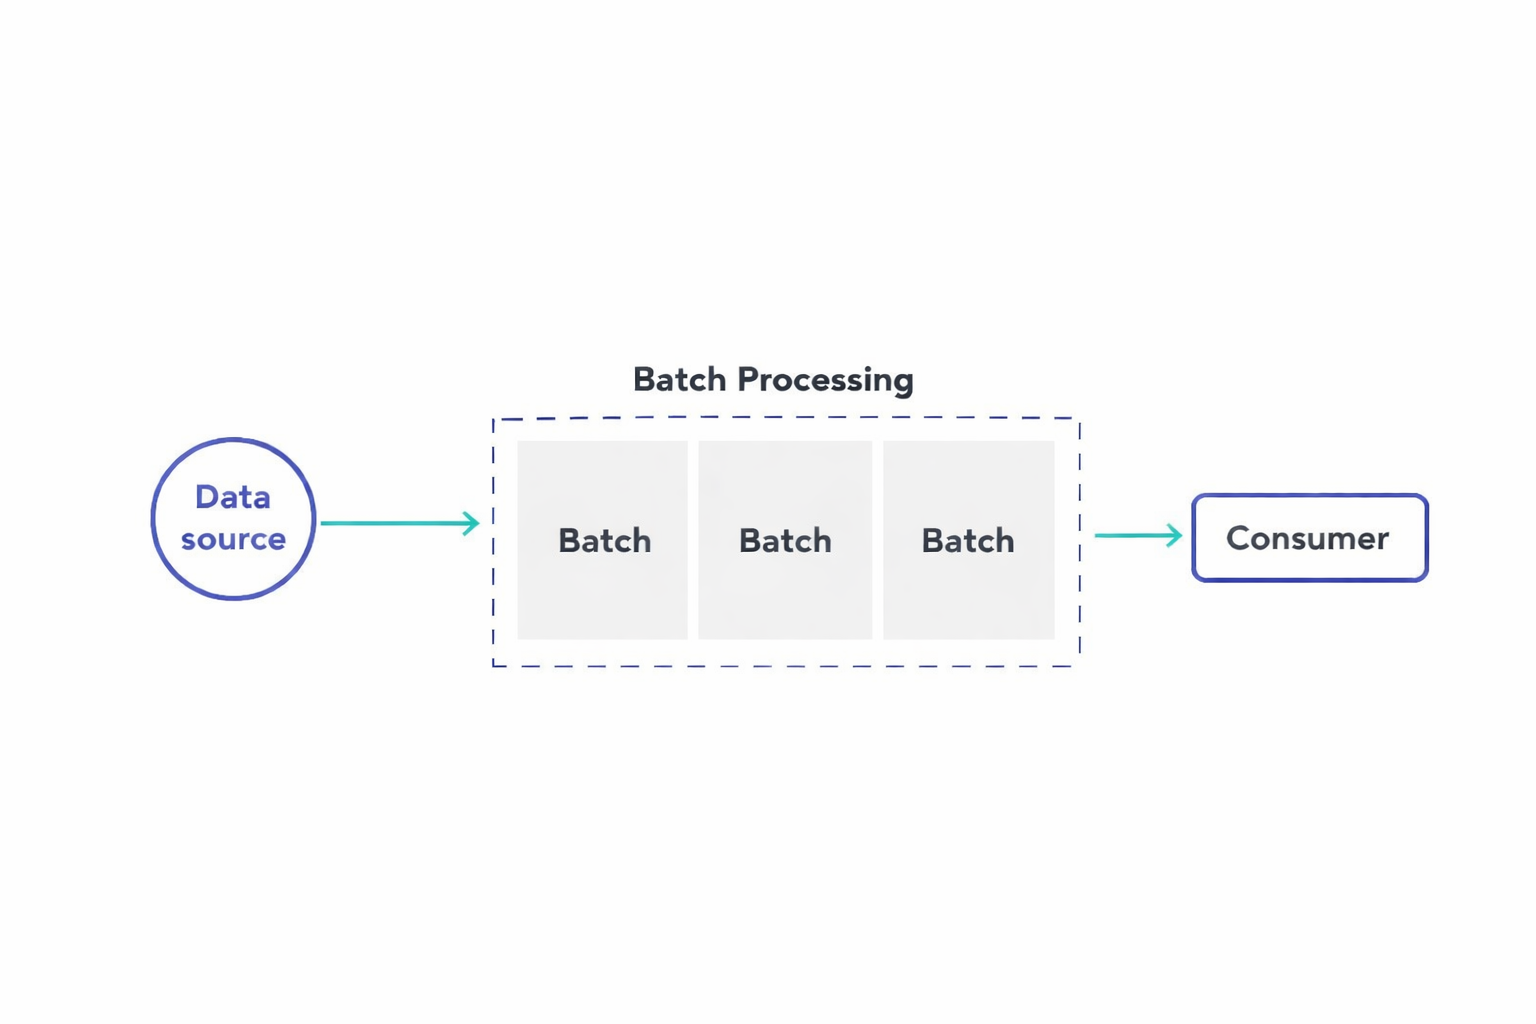
\includegraphics[width=0.85\textwidth]{II_2__micro_batch_processing.png}
    \caption{Micro-batch Processing}
    \label{fig:micro-batch-processing}
\end{figure}

\begin{quote}
Ukuran batch yang lebih besar cenderung meningkatkan efisiensi pemrosesan, tetapi juga menyebabkan event menunggu lebih lama sebelum diproses, sehingga latensi sinkronisasi meningkat. Sebaliknya, batch berukuran kecil dapat menurunkan latensi, tetapi meningkatkan overhead pemrosesan per event dan menurunkan efisiensi sistem. Kondisi ini menunjukkan adanya trade-off antara kecepatan propagasi data dan efisiensi pemrosesan, yang tidak dapat dioptimalkan secara bersamaan melalui satu konfigurasi statik (Kleppmann, 2017).

Backlog muncul ketika laju produksi event melebihi kemampuan sistem dalam memproses event tersebut. Backlog bersifat dinamis dan dipengaruhi oleh pola beban kerja, pengaturan batch, serta kondisi sumber daya pada sistem tujuan. Peningkatan backlog tidak hanya meningkatkan latensi sinkronisasi, tetapi juga berpotensi memicu lonjakan utilisasi CPU, memori, dan operasi I/O pada database baca ketika batch diproses dalam jumlah besar (Tanenbaum dan van Steen, 2017).

Penelitian terdahulu menunjukkan bahwa pengaturan batch secara statik sulit mempertahankan performa yang stabil pada kondisi beban yang berubah. Parameter batch yang optimal pada satu kondisi dapat menjadi tidak efektif pada kondisi lain, sehingga pengaturan batch dan pemantauan backlog perlu dipandang sebagai bagian dari sistem yang bersifat dinamis. Pandangan ini menjadi dasar untuk memodelkan proses sinkronisasi data sebagai sistem dinamis, yang membuka ruang bagi pendekatan pengendalian adaptif pada bab-bab selanjutnya (Wu dkk., 2020).
\end{quote}

\section{Pengendalian Umpan Balik dalam Sistem Perangkat Lunak}

\begin{quote}
Pengendalian umpan balik merupakan pendekatan yang digunakan untuk mengatur perilaku sistem agar tetap stabil dan optimal dengan menyesuaikan parameter-parameter kontrol berdasarkan pengamatan kondisi sistem dan deviasi dengan nilai yang diinginkan secara real-time (Ogata, 2010). Dalam konteks sistem sinkronisasi basis data, pengendalian umpan balik memungkinkan sistem untuk mengatur aspek-aspek seperti konsumsi sumber daya atau laju eksekusi proses mengikuti perubahan kondisi lingkungan seperti beban kerja maupun \emph{latency} dari infrastruktur.

Salah satu alasan pendekatan ini relevan dalam sistem perangkat lunak modern adalah karena sistem perangkat lunak modern semakin bersifat kompleks, sehingga konfigurasi secara static tidak dapat selalu menjadi yang optimal. Untuk mengatasi hal ini, digunakan sistem kontrol berbasis \emph{feedback loop} yang dapat bereaksi terhadap deviasi dari performa yang diinginkan. Pengendalian seperti ini telah diterapkan pada pengaturan throughput layanan cloud, alokasi dinamis memori, dan pengendalian autoscaling sistem.
\end{quote}

\subsection{Teori Kontrol pada Sistem Perangkat Lunak}

\begin{quote}
Teori kontrol merupakan disiplin ilmu yang membahas bagaimana suatu sistem dapat mengatur dirinya sendiri berdasarkan sinyal umpan balik (\emph{feedback}). Secara prinsip, teori kontrol bekerja dengan cara mengukur deviasi antara kondisi aktual sistem dengan kondisi yang diharapkan (\emph{setpoint}), lalu menghasilkan tindakan perbaikan untuk meminimalkan perbedaan tersebut (Ogata, 2010).

Dalam sistem perangkat lunak, sinyal umpan balik dapat berupa metrik runtime seperti penggunaan CPU, backlog antrian data, \emph{response time}. Dengan menggunakan pengendali yang sesuai, sistem dapat mengubah parameter konfigurasinya, seperti ukuran batch, atau frekuensi polling, agar kinerja sistem tetap stabil meskipun kondisi eksternal berubah. Pendekatan seperti ini sangat relevan dalam arsitektur modern yang bersifat elastis dan skalabel, serta ketika sistem perlu menyeimbangkan antara dua tujuan yang saling bertentangan misalnya performa dan konsistensi data.

Model formal dari sistem yang dikendalikan biasanya dinyatakan dalam bentuk \emph{state-space representation}, di mana sistem digambarkan sebagai hubungan linier antara status saat ini, aksi kontrol, dan status selanjutnya:

\[x_{t + 1} = Ax_{t} + Bu_{t}\]

\[y_{t} = Cx_{t} + Du_{t}\]

Dalam konteks sistem sinkronisasi data, status sistem \emph{x} dapat berupa utilitas cpu, jumlah antrian pesan, atau utilisasi memori, sedangkan \emph{u} adalah tindakan yang bisa diambil sistem seperti memperbesar batch atau memperpanjang interval polling. Matriks \emph{A} dan \emph{B} menggambarkan dinamika sistem, yaitu bagaimana sistem berubah sebagai akibat dari tindakan yang dilakukan. Sedangkan variabel pada vector \emph{y} dapat termati secara langsung dan biasanya merupakan \emph{subset} dari \emph{x}.

Dengan pendekatan ini, kita tidak hanya bereaksi terhadap kondisi saat ini, tetapi juga mengoptimalkan tindakan agar sistem tetap berada dalam kondisi yang stabil dan efisien. Di sinilah pendekatan kontrol optimal seperti LQR menjadi sangat relevan.
\end{quote}

\subsection{Linear Quadratic Regulator}

\begin{quote}
Linear Quadratic Regulator (LQR) adalah salah satu teknik pengendalian optimal yang terkenal dan banyak digunakan dalam dunia teknik kendali. Keunggulan utama dari LQR adalah kemampuannya untuk secara matematis menyeimbangkan antara dua tujuan yang sering bertentangan yaitu meminimalkan kesalahan sistem dan meminimalkan usaha kontrol.

Secara formal, LQR bertujuan untuk meminimalkan fungsi biaya kuadratik berikut ini:

\[J = \sum_{t = 0}^{\infty}{x_{t}^{T}Qx_{t} + u_{t}^{T}Ru_{t}}\]

Di mana:
\end{quote}

\begin{itemize}
\item \(J:\) fungsi biaya
\item \(x_{t}:\) status sistem saat ini (misalnya, antrian pesan atau tingkat utilisasi CPU),
\item \(u_{t}:\) sinyal kontrol (misalnya, pengaturan batch size, poll interval),
\item \(Q:\) bobot penalti terhadap kesalahan status sistem, berupa matriks definit positif,
\item \(R:\) bobot penalti terhadap usaha pengendalian, berupa matriks definit positif.
\end{itemize}

\begin{figure}[H]
    \centering
    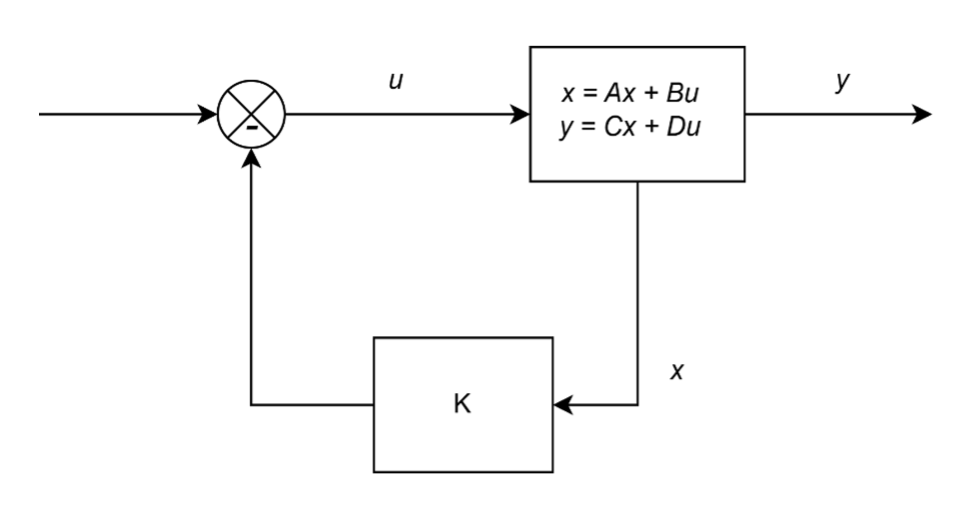
\includegraphics[width=0.75\textwidth]{II_3_1__kontrol_lqr.png}
    \caption{Kontrol LQR}
    \label{fig:kontrol-lqr}
\end{figure}

\begin{quote}
Solusi optimal dari fungsi biaya ini adalah hukum kontrol linier:

\[u_{t} = - Kx_{t}\]

dengan \emph{K} adalah matriks penguat (gain) yang diperoleh dari penyelesaian persamaan Riccati. Matriks ini menunjukkan seberapa besar tindakan korektif yang harus diambil untuk setiap kesalahan yang terdeteksi dalam status sistem.

Pendekatan LQR cocok digunakan untuk sistem yang kompleks, linear dan bersifat multi input dan multi output (MIMO). Dalam sistem sinkronisasi yang kompleks, kita mungkin perlu mengontrol beberapa parameter sekaligus seperti batch size dan interval polling. Keduanya menentukan multi variable kontrol dan tidak dapat diatur secara independen. Pada kasus seperti ini, LQR memberikan kerangka kerja matematis yang sistematis untuk merancang pengendali yang mempertimbangkan semua variabel sekaligus.

Namun, untuk menerapkan LQR, diperlukan pemodelan sistem terlebih dahulu. Hal ini dilakukan dengan cara melakukan eksperimen untuk merekam perubahan status sistem sebagai respons terhadap perubahan parameter kontrol, lalu menggunakan teknik estimasi seperti regresi linier atau metode identifikasi sistem (Ljung, 1999). Hasilnya berupa estimasi terhadap matriks A dan B, yang diperlukan untuk merancang kontroler LQR.

Walaupun implementasinya lebih kompleks dibandingkan pendekatan seperti PID, LQR menawarkan keunggulan dalam hal kestabilan, keoptimalan, dan fleksibilitas. Penentuan parameter kontrol pada LQR juga lebih sesuai untuk diterapkan pada kondisi berbasis \emph{trade-off} karena didasarkan pada matriks biaya yang bisa diatur untuk menentukan variabel mana yang akan diunggulkan dibanding yang lain. Oleh karena itu, dalam sistem yang memerlukan kontrol presisi tinggi terhadap dinamika kompleks seperti dalam pengelolaan sinkronisasi data yang adaptif dan berbasis resource utilization LQR merupakan pilihan yang sangat menjanjikan.
\end{quote}

\blankpage
\chapter{Analisis dan Solusi}

Fenomena ketidaksinkronan pada arsitektur CQRS muncul sebagai konsekuensi dari pemisahan model tulis dan baca yang bergantung pada aliran event.
Pada kondisi beban yang fluktuatif, laju kedatangan event tidak selalu sejalan dengan kapasitas pemrosesan konsumer, sehingga backlog dapat meningkat dan menghasilkan keterlambatan pembaruan pada database baca.
Peningkatan ukuran batch memang dapat menurunkan frekuensi pemrosesan dan mengurangi overhead, tetapi juga berpotensi menambah penundaan pembaruan data.
Sebaliknya, ukuran batch yang terlalu kecil menghasilkan pemrosesan yang lebih responsif, namun cenderung meningkatkan konsumsi sumber daya dan menurunkan throughput.

Untuk itu, diperlukan sistem yang mampu menyeimbangkan kebutuhan akan data yang responsif namun juga efisien dalam penggunaan sumber daya.
Dalam perancangan sistem tersebut, diperlukan pemahaman yang baik mengenai hubungan antara variabel-variabel yang membentuk dinamika sistem.
Analisis ini mencakup identifikasi variabel state yang mewakili kondisi sistem pada suatu waktu, variabel kontrol yang dapat diatur, serta bagaimana perubahan pada variabel tersebut memengaruhi performa sinkronisasi, baik dalam hal backlog, latensi, maupun utilisasi sumber daya.
Pemahaman ini menjadi dasar perumusan model pengendalian yang memungkinkan penyesuaian parameter secara adaptif agar sistem tetap berada pada kondisi yang stabil dan efisien.

\section{Analisis Masalah}

Alur sinkronisasi pada arsitektur CQRS bergantung pada proses konsumsi event dari log, pengelompokan event ke dalam batch, dan materialisasi ulang menjadi read model.
Pada kondisi beban rendah, alur ini cenderung stabil karena kapasitas pemrosesan sejalan dengan laju kedatangan event.
Namun ketika terjadi peningkatan throughput penulisan atau penurunan kapasitas konsumsi, backlog mulai meningkat dan menimbulkan keterlambatan propagasi data ke read model.
Keterlambatan ini dapat secara langsung dirasakan pengguna dalam hal ketidakakuratan data karena data yang tidak aktual.

Masalah menjadi lebih kompleks karena pengaturan parameter utama seperti ukuran batch dan interval polling tidak selalu menaikkan performa.
Ukuran batch yang lebih besar dapat meningkatkan efisiensi pemrosesan karena mengurangi frekuensi commit dan overhead jaringan dan komputasi, tetapi juga menunda waktu mulai pemrosesan sehingga menambah latensi sinkronisasi terlihat pada Gambar~\ref{fig:batch-latency}.
Sebaliknya, ukuran batch yang lebih kecil mempercepat pembaruan data tetapi meningkatkan konsumsi sumber daya CPU dan I/O, yang pada tingkat tertentu justru menurunkan throughput keseluruhan.
Ketidakseimbangan ini menyebabkan sistem rentan terhadap ketidakpastian performa ketika beban berubah-ubah, terutama pada skenario bersifat \emph{bursty}.

\begin{figure}[h]
    \centering
    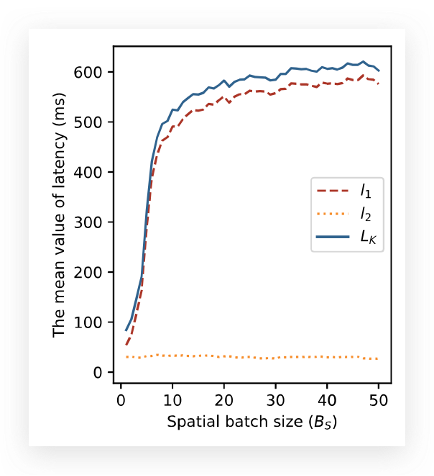
\includegraphics[width=0.85\textwidth]{III_1__scatter_batch_size.png}
    \caption{Pengaruh ukuran batch terhadap rata-rata \emph{latency} (Wu, 2020)}
    \label{fig:batch-latency}
\end{figure}

Untuk memahami perilaku sistem tersebut, beberapa variabel dapat dianggap sebagai representasi kondisi atau state sistem.
Backlog event menjadi indikator utama yang menggambarkan selisih antara laju produksi dan laju konsumsi pada saat itu.
Latensi pemrosesan event menunjukkan waktu yang dibutuhkan untuk memproses sebuah perubahan dan sangat dipengaruhi oleh besarnya batch, kapasitas komputasi, serta tingkat kontensi sumber daya.
Selain itu, utilisasi CPU atau memori pada komponen konsumer juga merefleksikan kapasitas sistem dalam merespons beban tambahan.
Variabel-variabel ini merepresentasikan kondisi sesaat sekaligus menentukan apakah sistem akan stabil atau terus menumpuk backlog.

Di sisi lain, variabel yang dapat dikendalikan atau \emph{control variables} meliputi ukuran batch dan interval polling pada konsumer.
Kedua parameter ini secara langsung mengatur ritme konsumsi data dan besarnya unit kerja yang diproses dalam setiap siklus.
Karena keduanya memengaruhi backlog, latensi, dan utilisasi sumber daya, kombinasi nilai yang tidak tepat dapat menyebabkan kondisi sistem berada di luar rentang yang diinginkan.
Masalah inilah yang ingin diatasi melalui pendekatan pengendalian dengan menentukan nilai pengaturan yang dapat menyeimbangkan pergerakan variabel state agar tetap berada pada kondisi stabil meskipun terjadi variasi beban.

Namun hubungan antara variabel state dan kontrol bersifat dinamis dan tidak selalu mudah dipetakan secara langsung.
Backlog, misalnya, bergantung pada interaksi antara laju produksi event dan kapasitas pemrosesan aktual pada konsumer, yang keduanya dapat bervariasi seiring waktu.
Latensi pemrosesan batch dapat berubah akibat peningkatan jumlah thread aktif, perubahan beban komputasi, atau efek kontensi I/O.
Ketidakpastian dan variasi inilah yang membuat pengaturan statis tidak memadai, karena parameter yang optimal pada satu kondisi dapat menjadi suboptimal atau bahkan kontraproduktif pada kondisi lainnya.
Oleh karena itu, diperlukan model yang mampu menangkap hubungan dinamis antara state dan kontrol sehingga sistem dapat diatur secara adaptif sesuai perubahan kondisi.

Analisis ini menunjukkan bahwa inti permasalahan bukan sekadar menentukan nilai batch atau interval polling yang paling cepat atau paling efisien, tetapi menemukan cara untuk menjaga keseimbangan antara backlog, latensi, dan utilisasi sumber daya dalam kondisi sistem yang terus berubah.
Model pengendalian dibutuhkan untuk menjaga agar variabel state bergerak menuju kondisi yang stabil dan terkendali, terlepas dari variasi beban.
Hasil analisis ini menjadi dasar perancangan pendekatan pengendalian pada bagian berikutnya.

\section{Analisis Solusi}

Berdasarkan analisis pada bagian sebelumnya, permasalahan sinkronisasi data pada arsitektur CQRS menunjukkan karakteristik sistem dinamis yang dipengaruhi oleh interaksi antara kondisi sistem dan parameter pengaturan pemrosesan.
Backlog, latensi sinkronisasi, dan utilisasi sumber daya tidak berkembang secara independen, melainkan saling mempengaruhi seiring perubahan beban dan konfigurasi sinkronisasi.
Oleh karena itu, solusi yang dirancang dalam penelitian ini tidak bertujuan mencari konfigurasi parameter statis yang optimal, melainkan mekanisme pengendalian yang mampu menyesuaikan parameter sinkronisasi secara adaptif agar sistem tetap berada pada kondisi seimbang.

Pendekatan pengendalian yang diusulkan dirancang dengan memformulasikan proses sinkronisasi sebagai sistem dinamis dalam kerangka \emph{state-space}.
Dengan formulasi ini, hubungan antara kondisi sistem (\emph{state}) dan parameter yang dapat dikendalikan (\emph{control input}) dapat dianalisis dan diatur secara sistematis.
Pendekatan ini memungkinkan penerapan berbagai strategi pengendalian, mulai dari kontrol umpan balik konvensional hingga kontrol optimal dan pendekatan berbasis data, dalam kerangka yang konsisten.

\subsection{Abstraksi Sistem dan Pemodelan State-Space}

Untuk merancang mekanisme pengendalian, proses sinkronisasi CQRS diabstraksikan sebagai sistem dinamis diskrit yang berevolusi seiring waktu.
Abstraksi ini memandang pipeline sinkronisasi, mulai dari konsumsi event hingga materialisasi \emph{read model}, sebagai sebuah sistem yang memiliki keadaan internal dan dapat dipengaruhi melalui aksi kontrol tertentu.
Pendekatan ini sejalan dengan praktik pemodelan sistem komputasi sebagai sistem dinamis ketika perilaku sistem dipengaruhi oleh umpan balik dan perubahan beban (Ogata, 2010).

Pada message sink, nilai-nilai matriks A, B, C, dan D diperoleh dari eksperimen dengan pendekatan \emph{open-loop} agar diketahui pengaruh variabel-variabel kontrol terhadap variabel-variabel state.
Eksperimen \emph{open-loop} adalah eksperimen yang menjalankan sistem tanpa kontroler aktif, sehingga parameter input divariasikan secara manual dan respons sistem dicatat apa adanya.
Lawannya adalah eksperimen \emph{closed-loop} yang menjalankan kontroler aktif sehingga parameter input ditentukan oleh kontroler berdasarkan kondisi sistem saat itu.
Vektor aksi kontrol didefinisikan sebagai:

\begin{equation}
\mathbf{u} = \begin{bmatrix} b \\ p \end{bmatrix}
\label{eq:vektor-kontrol}
\end{equation}

di mana:
\begin{enumerate}
\item $b$ adalah \emph{batch size}, yaitu jumlah pesan yang diproses dalam satu batch
\item $p$ adalah \emph{poll interval}, yaitu waktu jeda yang ditentukan untuk sistem dapat memproses batch data
\end{enumerate}

Vektor state $\mathbf{x}$ didefinisikan sebagai:

\begin{equation}
\mathbf{x} = \begin{bmatrix} n \\ c \\ m \\ o \end{bmatrix}
\label{eq:vektor-state}
\end{equation}

di mana:
\begin{enumerate}
\item $n$ adalah banyaknya pesan pada event source
\item $c$ adalah \emph{CPU utilization}
\item $m$ adalah \emph{memory utilization}
\item $o$ adalah \emph{I/O operation}
\end{enumerate}

Latensi sinkronisasi $l$ diperlakukan sebagai variabel observasi yang masuk ke matriks
output $C$ pada model state-space, bukan sebagai komponen vektor state.
Artinya, $l$ diukur untuk mengevaluasi kualitas sinkronisasi tetapi tidak digunakan oleh
kontroler untuk menentukan aksi koreksi.
Latensi diukur secara langsung melalui mekanisme \emph{manual offset commit} pada
\emph{message broker}.
Consumer tidak melakukan \emph{auto-commit} offset setelah mengambil batch, melainkan menunda
commit hingga \emph{read database} mengirimkan \emph{acknowledgement} yang mengonfirmasi
seluruh data dalam batch berhasil ditulis.
Latensi sinkronisasi untuk setiap batch dihitung sebagai:

\begin{equation}
l = t_{\text{ack}} - t_{\text{produce}}
\label{eq:latency-measurement}
\end{equation}

\noindent di mana $t_{\text{produce}}$ adalah waktu event diproduksi pada sisi tulis dan
$t_{\text{ack}}$ adalah waktu \emph{acknowledgement} diterima dari \emph{read database}.
Pendekatan ini memastikan latensi yang diukur mencakup seluruh waktu propagasi end-to-end,
termasuk waktu tunggu di antrian dan waktu pemrosesan batch.

Pemilihan variabel state didasarkan pada dua pertimbangan utama.
Pertama, variabel dapat diobservasi atau diukur secara real-time.
Kedua, variabel tersebut memiliki pengaruh langsung terhadap laju sinkronisasi dan tekanan
terhadap \emph{read database}.
Latensi tidak dimasukkan ke vektor state karena pengujian awal menunjukkan bahwa latensi di
state menyebabkan kontroler menekan \emph{batch size} secara berlebihan, sehingga latensi
hanya dijadikan variabel observasi terpisah.

Dalam konteks sistem nyata, hubungan antara \emph{state} dan \emph{control} bersifat nonlinier.
Namun, untuk keperluan perancangan kontrol optimal, sistem diasumsikan dapat didekati secara linier pada rentang operasi tertentu (\emph{linearization around operating point}).
Selain itu, diasumsikan bahwa perubahan beban dalam satu interval kontrol relatif kecil (\emph{quasi-stationary assumption}), sehingga pendekatan linier diskrit masih valid untuk perancangan kendali (Ogata, 2010; Hellerstein dkk., 2004).
Validitas asumsi ini kemudian diuji melalui eksperimen \emph{open-loop} pada tahap persiapan penelitian.

\subsection{Perancangan Fungsi Biaya dan Definisi Keseimbangan}

Tujuan pengendalian dalam penelitian ini adalah mengompromikan kecepatan sinkronisasi data dengan efisiensi penggunaan sumber daya.
Kompromi ini tidak dapat diwakili oleh satu metrik tunggal, karena melibatkan beberapa tujuan yang saling bertentangan, seperti minimisasi backlog, pengurangan latensi sinkronisasi, dan pembatasan utilisasi sumber daya agar tidak melampaui kapasitas sistem (Bailis dkk., 2012).

Untuk merepresentasikan tujuan tersebut secara formal, digunakan fungsi biaya kuadratik:

\begin{equation}
J = \sum_{t=0}^{\infty} \left( x_t^T Q x_t + u_t^T R u_t \right)
\label{eq:fungsi-biaya}
\end{equation}

Pada setiap langkah waktu $t$, vektor state $x_t$ berisi kondisi aktual sistem, yaitu jumlah backlog, utilisasi CPU, utilisasi memori, dan intensitas operasi I/O saat itu.
Masing-masing komponen $x_t$ dikuadratkan dan dikalikan dengan bobot yang ditetapkan di matriks $Q$.
Jika backlog saat ini adalah 3.000 dan target adalah 0, maka backlog berkontribusi pada biaya sebesar $3000^2 \times Q[\text{backlog}]$.
Hal yang sama berlaku untuk setiap variabel state lainnya.
Secara bersamaan, aksi kontrol yang diterapkan ($u_t$, yaitu batch size dan poll interval yang dipilih) juga dihitung biayanya melalui matriks $R$, agar sistem tidak mengambil tindakan yang terlalu ekstrem.
Nilai dari kedua komponen ini dijumlahkan untuk setiap langkah waktu, dan total akumulasinya itulah yang membentuk $J$.
Komponen pertama dari fungsi biaya dengan demikian memberikan penalti terhadap deviasi kondisi sistem dari keadaan yang diinginkan, sementara komponen kedua memberikan penalti terhadap besarnya aksi kontrol yang diterapkan.
Dengan formulasi ini, sistem diarahkan untuk mengurangi backlog dan utilisasi sumber daya sekaligus menghindari perubahan parameter sinkronisasi yang terlalu agresif maupun terlalu lambat.

Makna optimal dalam kerangka LQR didefinisikan sebagai keputusan kontrol yang meminimalkan fungsi biaya tersebut sepanjang horizon waktu, sehingga menghasilkan kompromi terbaik antara perbaikan kondisi sistem dan besarnya perubahan parameter sinkronisasi.
Bobot pada matriks $Q$ mencerminkan tingkat kepentingan relatif masing-masing variabel state, misalnya penekanan yang lebih besar pada backlog akan mendorong sistem untuk mempercepat sinkronisasi, sementara penekanan pada utilisasi sumber daya akan menghasilkan perilaku pengendalian yang lebih konservatif.
Matriks $R$ berfungsi untuk membatasi perubahan \emph{batch size} dan \emph{poll interval} agar tidak terlalu agresif, sehingga mengurangi potensi osilasi dan ketidakstabilan sistem.

\subsection{Kontrol Optimal Linear Quadratic Regulator (LQR)}

Kontrol optimal LQR digunakan sebagai pendekatan berbasis model yang secara eksplisit memformulasikan tujuan pengendalian dalam bentuk fungsi biaya.
LQR bekerja berdasarkan representasi \emph{state-space} sistem, di mana kondisi sinkronisasi direpresentasikan sebagai vektor state dan parameter sinkronisasi sebagai vektor kontrol.
Dengan model ini, LQR menghitung kebijakan kontrol yang meminimalkan fungsi biaya kuadratik yang merepresentasikan keseimbangan antara perbaikan kondisi sistem dan besarnya aksi kontrol.

Solusi optimal dari fungsi biaya ini adalah hukum kontrol linier:

\begin{equation}
u_t = -K x_t
\label{eq:hukum-kontrol}
\end{equation}

dengan $K$ adalah matriks penguat (gain) yang diperoleh dari penyelesaian persamaan Riccati.
Matriks ini menunjukkan seberapa besar tindakan korektif yang harus diambil untuk setiap kesalahan yang terdeteksi dalam status sistem.

LQR mempertimbangkan seluruh variabel state secara simultan dan tidak hanya berfokus pada satu sinyal kesalahan.
Pendekatan ini memungkinkan pengendalian yang lebih sistematis terhadap trade-off antara backlog, latensi sinkronisasi, dan utilisasi sumber daya.
Kebijakan kontrol LQR diperoleh melalui penyelesaian persamaan Riccati, sehingga aksi kontrol yang dihasilkan bersifat optimal secara matematis pada asumsi linearitas lokal dan gangguan terbatas.

Keterbatasan utama LQR terletak pada kebutuhan akan model sistem dan penentuan bobot fungsi biaya yang tepat.
Proses identifikasi model dan penalaan bobot memerlukan eksperimen awal dan pemahaman terhadap dinamika sistem.
Meskipun demikian, LQR memberikan kerangka pengendalian yang interpretable dan konsisten secara teori, sehingga cocok digunakan sebagai pendekatan utama dalam penelitian ini.

\subsection{Pendekatan Pengendalian yang Dibandingkan}

Untuk mengevaluasi efektivitas LQR secara menyeluruh, penelitian ini membandingkan empat pendekatan pengendalian yang merepresentasikan spektrum dari tanpa kontrol hingga kontrol optimal berbasis model.
Keempat pendekatan ini (statik, berbasis aturan, PID, dan LQR) menggunakan abstraksi sistem dan fungsi biaya yang sama sebagaimana didefinisikan pada Persamaan~\ref{eq:vektor-kontrol}--\ref{eq:vektor-state} dan Persamaan~\ref{eq:fungsi-biaya}, sehingga perbandingan dilakukan pada kerangka evaluasi yang konsisten.

\subsubsection{Kontrol Statik (Fixed)}

Pendekatan kontrol statik menggunakan nilai batch size dan poll interval yang tetap sepanjang eksperimen.
Nilai parameter ditentukan berdasarkan rata-rata kondisi operasional normal yang diperoleh dari eksperimen open-loop.
Pendekatan ini berfungsi sebagai baseline untuk menunjukkan kebutuhan akan mekanisme pengendalian adaptif.
Tanpa kemampuan menyesuaikan parameter terhadap perubahan beban, kontrol statik diharapkan menunjukkan kinerja yang menurun secara signifikan ketika kondisi operasional menyimpang dari asumsi awal.

\subsubsection{Kontrol Berbasis Aturan (Rule-Based)}

Pendekatan berbasis aturan menggunakan sekumpulan aturan threshold untuk menyesuaikan parameter sinkronisasi.
Aturan dirancang berdasarkan pemahaman domain tentang hubungan antara variabel state dan parameter kontrol.
Sebagai contoh, ketika backlog melebihi batas tertentu, batch size diperbesar untuk meningkatkan laju konsumsi; ketika utilisasi CPU melebihi ambang yang ditentukan, batch size dikurangi untuk menghindari kelebihan beban.

Pendekatan ini merepresentasikan praktik umum dalam pengelolaan sistem perangkat lunak, di mana administrator menetapkan aturan penyesuaian berdasarkan pengalaman operasional.
Keterbatasan utama pendekatan ini adalah ketidakmampuannya mempertimbangkan interaksi antar variabel secara simultan dan tidak adanya definisi formal mengenai keseimbangan yang ingin dicapai.

\subsubsection{Kontrol PID}

Kontrol PID diterapkan sebagai pendekatan kontrol klasik yang menggunakan satu sinyal kesalahan untuk menghasilkan aksi koreksi.
Dalam penelitian ini, PID dikonfigurasi sebagai kontroler single-loop dengan backlog sebagai variabel yang dikendalikan dan batch size sebagai variabel kontrol.
Sinyal kesalahan dihitung sebagai selisih antara nilai backlog aktual dan nilai referensi yang diinginkan.

Parameter $K_p$, $K_i$, dan $K_d$ ditentukan melalui metode tuning berdasarkan data eksperimen open-loop.
PID berfungsi sebagai representasi pendekatan kontrol klasik yang sudah mapan, dengan keterbatasan utama pada sifat SISO yang hanya mengamati satu variabel state dan mengendalikan satu variabel kontrol, tanpa memperhitungkan trade-off multi-variabel secara eksplisit.

\section{Rancangan Solusi}

Persiapan penelitian dilakukan untuk memperoleh data yang merepresentasikan dinamika sinkronisasi sistem pada berbagai kondisi beban.
Data ini digunakan untuk identifikasi hubungan antara kondisi sistem dan parameter sinkronisasi, serta sebagai dasar pelatihan model pembelajaran berbasis data.
Seluruh proses persiapan dirancang agar konsisten dengan tujuan pengendalian dan metrik evaluasi yang digunakan pada tahap pengujian.

\subsection{Eksperimen Open-Loop dan Identifikasi Sistem}

Eksperimen open-loop dilakukan dengan menjalankan sistem sinkronisasi tanpa mekanisme pengendalian adaptif aktif.
Parameter sinkronisasi diatur secara manual dan divariasikan dalam rentang yang telah ditentukan, sementara kondisi sistem diamati dan dicatat secara periodik.
Pendekatan ini dipilih untuk memastikan bahwa hubungan sebab akibat antara parameter sinkronisasi dan respons sistem dapat diamati secara langsung, tanpa dipengaruhi oleh umpan balik pengendali.

Pada setiap interval pengamatan, kondisi sistem dicatat sebagai vektor state yang mencakup backlog event, utilisasi CPU, utilisasi memori, dan intensitas operasi I/O pada read database.
Secara bersamaan, parameter kontrol berupa batch size dan poll interval dicatat sebagai bagian dari konfigurasi eksperimen.
Pengukuran dilakukan pada interval waktu yang tetap untuk menjaga konsistensi temporal antar variabel.

Eksperimen dijalankan pada beberapa skenario beban yang berbeda, termasuk beban rendah, sedang, dan tinggi.
Untuk setiap skenario, beberapa kombinasi parameter sinkronisasi diuji dan dijalankan selama jendela waktu observasi yang sama.
Selama periode tersebut, metrik performa seperti perubahan backlog, latensi sinkronisasi, dan utilisasi sumber daya dicatat untuk dianalisis lebih lanjut.
Data tersebut dimanfaatkan untuk mengamati karakteristik dinamika sistem dan merancang matriks kontrol.

\subsection{Definisi Aksi Kontrol Optimal}

Aksi kontrol optimal $u^*(t)$ didefinisikan sebagai parameter sinkronisasi yang menghasilkan kinerja terbaik untuk suatu kondisi sistem tertentu berdasarkan tujuan pengendalian yang telah ditetapkan.
Dalam penelitian ini, definisi optimal tidak diartikan sebagai minimisasi satu metrik secara terpisah, melainkan sebagai pencapaian keseimbangan antara backlog, latensi sinkronisasi, dan pemanfaatan sumber daya dalam suatu horizon pengamatan yang terbatas.

Secara formal, untuk kondisi sistem $x(t)$, aksi kontrol optimal didefinisikan sebagai:

\begin{equation}
u^*(t) = \arg\min_{u \in \mathcal{U}} J(u, x(t))
\label{eq:aksi-optimal}
\end{equation}

di mana $\mathcal{U}$ adalah himpunan kandidat aksi kontrol yang memenuhi batas operasional sistem, dan $J$ adalah fungsi biaya yang merepresentasikan tujuan pengendalian sesuai dengan Persamaan~\ref{eq:fungsi-biaya}.

Pada suatu kondisi awal sistem yang diamati, beberapa kombinasi parameter sinkronisasi, yaitu batch size dan poll interval, diuji secara terpisah.
Selama satu periode pengamatan, aksi kontrol dijaga tetap konstan untuk setiap kombinasi yang diuji, sementara respons sistem dicatat secara periodik.
Nilai fungsi biaya kemudian dihitung dari respons tersebut, dan kombinasi parameter yang menghasilkan nilai fungsi biaya minimum ditetapkan sebagai aksi kontrol optimal untuk kondisi sistem tersebut.

Pendekatan ini memastikan bahwa definisi $u^*(t)$ konsisten dengan tujuan pengendalian LQR, meskipun diperoleh melalui evaluasi empiris.
Dengan demikian, $u^*(t)$ menjadi aksi kontrol paling seimbang untuk kondisi sistem tertentu dalam batas asumsi dan horizon pengamatan yang berlaku, dan menjadi acuan pada analisis performa serta perbandingan di tahap evaluasi.

\section{Desain Eksperimen dan Skenario Pengujian}

Desain eksperimen pada penelitian ini bertujuan untuk mengevaluasi efektivitas pengendalian sinkronisasi data berbasis LQR dalam berbagai kondisi operasional sistem.
Eksperimen dirancang agar hasil yang diperoleh mencerminkan pengaruh mekanisme pengendalian, bukan faktor eksternal lainnya.

Eksperimen dilakukan dengan menjalankan sistem CQRS pada lingkungan uji yang konsisten, dengan konfigurasi perangkat keras, skema data, dan logika materialisasi read model yang dijaga tetap.
Variasi yang diperkenalkan dalam eksperimen dibatasi pada skenario beban dan parameter pengendalian yang menjadi fokus penelitian.
Pendekatan ini memastikan validitas internal eksperimen dan memungkinkan interpretasi hasil yang lebih jelas.

\subsection{Lingkungan Uji}

Lingkungan uji dirancang untuk merepresentasikan kondisi operasional sistem sinkronisasi data berbasis CQRS secara realistis dan terkontrol.
Seluruh eksperimen dijalankan pada arsitektur yang sama untuk memastikan bahwa perbedaan kinerja yang diamati berasal dari mekanisme pengendalian, bukan dari perubahan konfigurasi sistem atau lingkungan eksekusi.

Arsitektur sistem uji terdiri dari empat komponen utama, yaitu write model sebagai sumber perubahan data, message broker sebagai media distribusi event, message sink sebagai konsumer event sekaligus titik penerapan kontrol, dan read database sebagai target materialisasi data.
Alur sinkronisasi dimulai dari operasi tulis pada write model yang menghasilkan event perubahan data, kemudian event tersebut dipublikasikan ke message broker dan dikonsumsi oleh message sink untuk diproses secara bertahap sebelum diterapkan ke read database.

\begin{figure}[H]
    \centering
    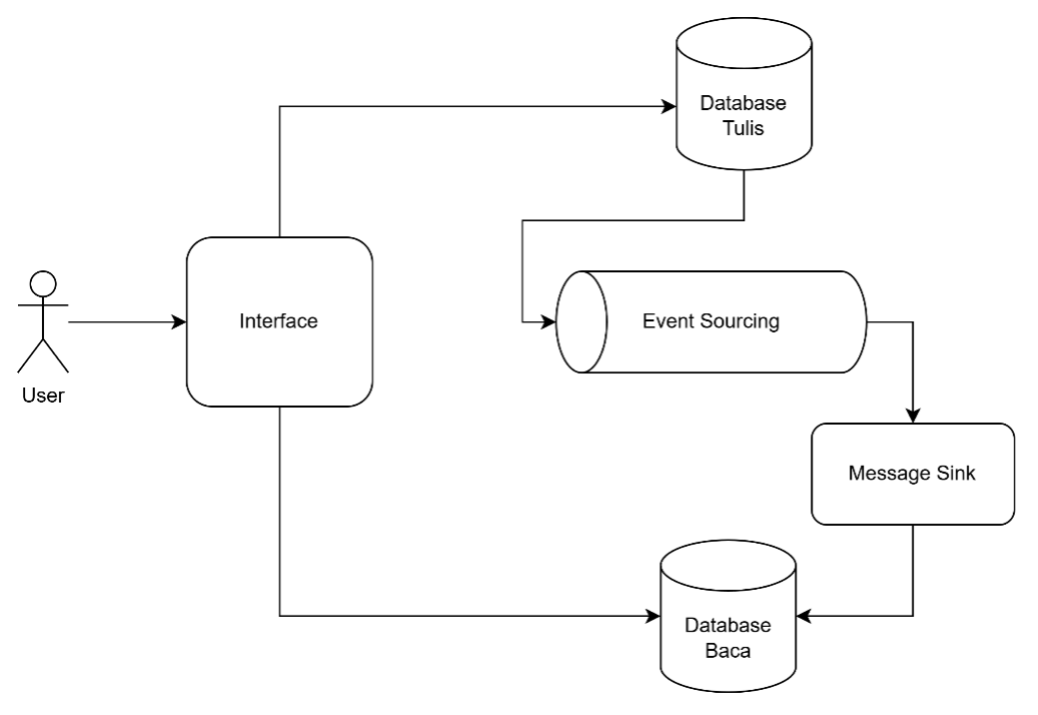
\includegraphics[width=0.9\textwidth]{III_4_1__arsitektur_uji.png}
    \caption{Arsitektur Desain yang akan diuji}
    \label{fig:arsitektur-desain}
\end{figure}

Mekanisme kontrol LQR ditempatkan pada message sink karena komponen ini memiliki peran langsung dalam menentukan laju konsumsi event dan intensitas beban yang diberikan ke read database.
Parameter sinkronisasi yang dikendalikan meliputi batch size dan poll interval, yang secara langsung memengaruhi jumlah event yang diproses dalam satu siklus serta frekuensi pemrosesan.
Dengan menempatkan kontrol pada message sink, sistem memperoleh fleksibilitas untuk menyesuaikan laju sinkronisasi tanpa mengganggu logika bisnis pada write model maupun pola akses pada sisi baca.

Selama eksperimen, konfigurasi perangkat keras dan perangkat lunak dijaga tetap.
Kapasitas CPU, memori, dan penyimpanan tidak diubah, demikian pula versi sistem operasi, message broker, dan basis data yang digunakan.
Skema data pada write model dan read database serta logika materialisasi data juga tidak mengalami perubahan.
Pendekatan ini dilakukan untuk menjaga validitas internal eksperimen dan memastikan bahwa dinamika sistem yang diamati mencerminkan pengaruh pengendalian terhadap proses sinkronisasi.

Sebelum setiap eksperimen dimulai, sistem dijalankan hingga mencapai kondisi awal yang stabil dengan konfigurasi parameter sinkronisasi default.
Periode stabilisasi ini bertujuan untuk menghindari pengaruh transien awal sistem terhadap hasil pengukuran.
Setelah kondisi awal tercapai, mekanisme kontrol LQR diaktifkan dan eksperimen dijalankan sesuai dengan skenario beban yang telah ditentukan.

\subsection{Perancangan Skenario Beban}

Skenario beban dirancang untuk mengevaluasi kinerja pengendalian sinkronisasi data berbasis LQR pada berbagai kondisi operasional dan pola perubahan beban.
Selain variasi tingkat beban, penelitian ini juga mempertimbangkan karakteristik temporal perubahan beban karena respons sistem kendali sangat dipengaruhi oleh bagaimana beban berubah terhadap waktu.

Skenario beban dengan pola \emph{step} digunakan untuk merepresentasikan perubahan beban yang terjadi secara tiba-tiba, misalnya lonjakan laju produksi event akibat peningkatan trafik secara mendadak.
Pola ini digunakan untuk mengamati respons transien sistem, khususnya waktu respons awal, kenaikan backlog, dan kemampuan pengendalian dalam meredam lonjakan beban secara cepat.

Pola \emph{ramp} digunakan untuk merepresentasikan perubahan beban yang meningkat atau menurun secara bertahap.
Pola ini mencerminkan kondisi pertumbuhan trafik yang progresif dan memungkinkan evaluasi kemampuan pengendalian dalam menyesuaikan parameter sinkronisasi secara gradual tanpa menimbulkan osilasi yang berlebihan.

Pola \emph{impulse} digunakan untuk merepresentasikan lonjakan beban sesaat dengan durasi singkat (\emph{short burst}), yang kemudian diikuti oleh kembalinya beban ke kondisi awal.
Pola ini bertujuan untuk mengamati sensitivitas sistem terhadap gangguan sementara dan kemampuan pengendalian dalam memulihkan kondisi sistem setelah gangguan terjadi.

Selain itu, digunakan pola \emph{step periodik} untuk merepresentasikan perubahan beban yang berulang antara dua tingkat tertentu dalam interval waktu tetap.
Pola ini digunakan untuk mengevaluasi stabilitas jangka menengah sistem pengendalian serta potensi munculnya osilasi akibat perubahan beban yang berulang.
Pengamatan pada skenario ini difokuskan pada konsistensi respons sistem dan kemampuan pengendalian dalam mempertahankan performa yang stabil pada siklus beban yang berulang.

Terakhir, pola \emph{step low} digunakan untuk merepresentasikan kondisi beban rendah yang konstan (100 msg/s), berbeda dengan pola \emph{step} yang menggunakan rate jauh lebih tinggi.
Pola ini berguna untuk menguji apakah kontroler tetap stabil saat antrean sangat kecil dan tidak bereaksi berlebihan ketika sistem sebenarnya dalam kondisi tenang.

Dengan menggunakan kombinasi kelima pola beban tersebut, eksperimen dapat menguji respons dan stabilitas pengendalian pada berbagai kondisi operasional.

\begin{figure}[H]
    \centering
    \begin{tabular}{cc}
        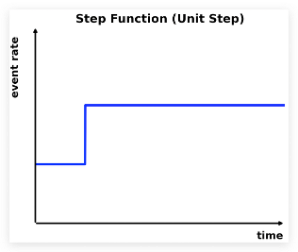
\includegraphics[width=0.48\textwidth]{III_4_2_a__skenario_step.png} &
        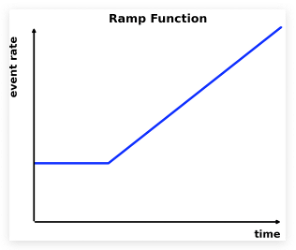
\includegraphics[width=0.48\textwidth]{III_4_2_b__skenario_ramp.png} \\
        (a) Fungsi Step & (b) Fungsi Ramp \\[0.5cm]
        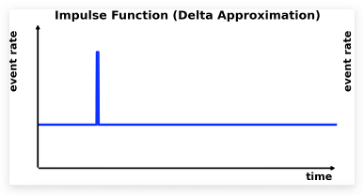
\includegraphics[width=0.48\textwidth]{III_4_2_c__skenario_impulse.png} &
        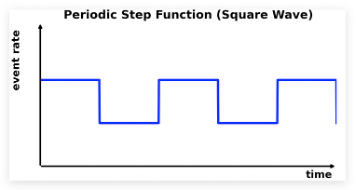
\includegraphics[width=0.48\textwidth]{III_4_2_d__skenario_periodic.png} \\
        (c) Fungsi Impulse & (d) Fungsi Step Periodik
    \end{tabular}
    \caption[Simulasi beban dengan beberapa skenario fungsi]{Simulasi beban dengan beberapa skenario fungsi (a) fungsi step, (b) fungsi ramp, (c) fungsi impulse dan (d) fungsi step yang berulang}
    \label{fig:skenario-beban}
\end{figure}

\subsection{Perancangan Eksperimen Perbandingan Metode}

Untuk memastikan keadilan perbandingan, seluruh pendekatan pengendalian dijalankan pada skenario beban yang sama dengan kondisi awal sistem yang identik.
Setiap metode menerima informasi state yang sama pada setiap interval kontrol dan menghasilkan aksi kontrol sesuai mekanismenya masing-masing.
Interval pengambilan keputusan kontrol dijaga tetap untuk seluruh metode agar perbedaan kinerja yang diamati berasal dari strategi pengendalian, bukan dari perbedaan frekuensi pengambilan keputusan.

Konfigurasi masing-masing metode ditentukan sebagai berikut.
Kontrol statik menggunakan nilai batch size dan poll interval yang ditetapkan berdasarkan rata-rata parameter pada kondisi beban normal dari data eksperimen open-loop.
Kontrol berbasis aturan menggunakan sekumpulan aturan threshold yang dirancang berdasarkan hubungan antar variabel yang teramati pada eksperimen open-loop, dengan batas threshold ditentukan dari distribusi nilai variabel state selama eksperimen.
Kontrol PID dikonfigurasi sebagai kontroler single-loop pada variabel backlog, dengan parameter $K_p$, $K_i$, dan $K_d$ ditentukan melalui metode tuning berbasis data eksperimen open-loop.
Kontrol LQR menggunakan matriks $A$ dan $B$ yang diidentifikasi dari eksperimen open-loop, serta matriks $Q$ dan $R$ yang mencerminkan prioritas pengendalian yang telah ditetapkan pada Persamaan~\ref{eq:fungsi-biaya}.

Setiap metode dijalankan pada kelima skenario beban (step, ramp, impulse, step periodik, dan step low) dengan durasi eksperimen yang sama.
Hasil eksperimen dievaluasi menggunakan seluruh metrik yang telah didefinisikan pada bagian III.5, sehingga perbandingan mencakup aspek kinerja sinkronisasi, dinamika kontrol, efisiensi pemrosesan, dan biaya kontrol.

\section{Metrik Evaluasi Kerja}

Evaluasi kinerja pada penelitian ini menilai sejauh mana pengendali menyeimbangkan kualitas sinkronisasi data dengan efisiensi penggunaan sumber daya.
Oleh karena itu, metrik evaluasi dipilih secara selektif agar dapat merepresentasikan tujuan pengendalian yang telah dirumuskan pada tahap perancangan solusi, serta mampu menangkap respons sistem pada berbagai kondisi beban dan pola perubahan beban.

Metrik evaluasi dikelompokkan berdasarkan perannya dalam analisis kinerja sistem, meliputi metrik inti kinerja sinkronisasi, metrik dinamika kontrol, metrik efisiensi pemrosesan, dan metrik biaya kontrol.
Pengelompokan ini bertujuan untuk memisahkan pengukuran kualitas sinkronisasi, karakteristik respons dinamis, efisiensi operasional, dan kesesuaian solusi terhadap formulasi optimasi yang digunakan.
Seluruh metrik diukur secara periodik selama eksperimen dan digunakan secara konsisten sebagai dasar analisis dan perbandingan keempat pendekatan pengendalian pada bab hasil dan pembahasan.

\subsection{Metrik Inti Kinerja Sinkronisasi}

Kelompok metrik inti ini menilai kualitas dasar proses sinkronisasi data pada arsitektur CQRS.
Metrik ini dipilih karena secara langsung merepresentasikan tujuan utama pengendalian, yaitu menjaga konsistensi data dan kestabilan sistem pada berbagai kondisi beban.
Seluruh metrik inti diukur secara periodik selama eksperimen dan dianalisis baik pada kondisi tunak maupun transien.

Backlog sinkronisasi digunakan sebagai indikator utama untuk mengukur tingkat ketertinggalan proses sinkronisasi.
Backlog didefinisikan sebagai jumlah event yang telah dihasilkan oleh write model tetapi belum diproses oleh message sink pada suatu waktu tertentu.
Nilai backlog yang tinggi menunjukkan ketidakseimbangan antara laju produksi dan konsumsi event, sedangkan pengendalian yang efektif ditunjukkan oleh kemampuan menekan pertumbuhan backlog dan mempercepat pemulihannya setelah terjadi gangguan.
Backlog diukur dalam satuan jumlah event, dengan analisis mencakup nilai rata-rata, nilai maksimum, dan waktu pemulihan menuju kondisi referensi.

Latensi sinkronisasi digunakan untuk mengukur keterlambatan propagasi perubahan data dari write model hingga perubahan tersebut tersedia pada read database.
Latensi ini mencerminkan konsistensi data yang dapat diamati oleh pengguna dan berhubungan langsung dengan kualitas layanan sistem.
Pengukuran latensi dilakukan dengan mencatat selisih waktu antara timestamp event pada sisi tulis dan waktu penerapan perubahan pada sisi baca.
Satuan yang digunakan adalah milidetik atau detik, dengan analisis meliputi nilai rata-rata dan nilai maksimum selama periode eksperimen.

Utilisasi sumber daya digunakan untuk mengevaluasi dampak pengendalian terhadap kapasitas sistem, khususnya pada komponen read database yang menjadi target materialisasi data.
Metrik ini mencakup utilisasi CPU, penggunaan memori, dan aktivitas I/O selama proses sinkronisasi berlangsung.
Utilisasi CPU dan memori diukur dalam persen, sedangkan aktivitas I/O diukur dalam operasi per detik atau jumlah data yang diproses per satuan waktu.
Metrik ini digunakan untuk memastikan bahwa pengendalian mampu menjaga keseimbangan antara peningkatan laju sinkronisasi dan keterbatasan sumber daya sistem.

\begin{table}[H]
    \centering
    \caption{Metrik kinerja sinkronisasi}
    \label{tab:metrik-sinkronisasi}
    \renewcommand{\arraystretch}{1.4}
    \begin{tabular}{|c|p{3cm}|p{6cm}|p{2.5cm}|}
    \hline
    \textbf{No} & \textbf{Metrik} & \textbf{Definisi Operasional} & \textbf{Satuan} \\
    \hline
    1 & Backlog Sinkronisasi & Jumlah event yang telah dihasilkan oleh write model tetapi belum diproses oleh message sink pada waktu tertentu & Event \\
    \hline
    2 & Backlog Rata-rata & Nilai rata-rata backlog selama satu periode eksperimen & Event \\
    \hline
    3 & Backlog Maksimum & Nilai backlog tertinggi yang tercatat selama eksperimen & Event \\
    \hline
    4 & Waktu Pemulihan Backlog & Waktu yang dibutuhkan backlog untuk kembali mendekati nilai referensi setelah terjadi gangguan beban & Detik \\
    \hline
    5 & Latensi Sinkronisasi Rata-rata & Rata-rata waktu dari event dihasilkan hingga diterapkan pada read database & Milidetik/detik \\
    \hline
    6 & Latensi Sinkronisasi Maksimum & Nilai latensi sinkronisasi tertinggi selama eksperimen & Milidetik/detik \\
    \hline
    7 & Utilisasi CPU & Persentase penggunaan CPU pada read database selama proses sinkronisasi & Persen \\
    \hline
    8 & Utilisasi Memori & Persentase penggunaan memori pada read database selama proses sinkronisasi & Persen \\
    \hline
    9 & Aktivitas I/O & Intensitas operasi baca tulis selama proses sinkronisasi & Persen \\
    \hline
    \end{tabular}
\end{table}

\subsection{Metrik Dinamika Kontrol}

Kelompok metrik dinamika kontrol menilai karakteristik respons sistem terhadap perubahan beban, terutama pada kondisi transien seperti pola step, ramp, impulse, dan step periodik.
Berbeda dengan metrik inti yang menilai kualitas sinkronisasi secara umum, metrik dinamika kontrol berfokus pada bagaimana sistem bereaksi terhadap gangguan dan seberapa cepat sistem kembali ke kondisi yang diinginkan.
Metrik ini sangat relevan dalam konteks pengendalian berbasis LQR karena secara langsung mencerminkan kualitas respons kendali yang dihasilkan.

Evaluasi dinamika kontrol dilakukan dengan mengamati perilaku temporal backlog sebagai variabel state utama.
Respons backlog terhadap perubahan beban digunakan untuk menilai kecepatan respons, tingkat agresivitas pengendalian, dan kestabilan menuju kondisi referensi.
Dengan menggunakan metrik dinamika kontrol, penelitian ini dapat membedakan pengendalian yang cepat namun berisiko agresif dari pengendalian yang lebih stabil dan terkontrol.

Rise time digunakan untuk mengukur kecepatan respons pengendalian terhadap gangguan beban.
Nilai rise time yang kecil menunjukkan bahwa mekanisme kontrol mampu merespons perubahan kondisi sistem secara cepat.
Namun, respons yang terlalu cepat dapat meningkatkan risiko overshoot, sehingga rise time perlu dianalisis bersamaan dengan metrik lainnya.

Overshoot merepresentasikan tingkat agresivitas pengendalian setelah terjadi perubahan beban.
Overshoot yang besar menunjukkan bahwa pengendalian memberikan respons berlebihan, yang berpotensi meningkatkan tekanan terhadap sistem.
Dalam konteks sinkronisasi data, overshoot backlog yang tinggi dapat mengindikasikan risiko overload sementara pada read database.

Settling time digunakan untuk mengevaluasi kestabilan respons pengendalian.
Metrik ini menunjukkan berapa lama sistem membutuhkan waktu untuk kembali dan bertahan pada kondisi yang mendekati nilai referensi setelah gangguan terjadi.
Settling time yang singkat tanpa overshoot berlebihan menunjukkan karakteristik pengendalian yang stabil dan efektif.

\begin{table}[H]
    \centering
    \caption{Metrik dinamika kontrol}
    \label{tab:metrik-dinamika}
    \renewcommand{\arraystretch}{1.4}
    \begin{tabular}{|c|p{3cm}|p{6cm}|p{2.5cm}|}
    \hline
    \textbf{No} & \textbf{Metrik} & \textbf{Definisi Operasional} & \textbf{Satuan} \\
    \hline
    1 & Rise Time & Waktu yang dibutuhkan backlog untuk kembali mendekati nilai referensi setelah terjadi perubahan beban & Detik \\
    \hline
    2 & Overshoot & Selisih maksimum backlog yang melebihi nilai referensi setelah terjadi perubahan beban & Persen \\
    \hline
    3 & Settling Time & Waktu yang dibutuhkan hingga backlog berada dan bertahan dalam rentang toleransi tertentu di sekitar nilai referensi & Detik \\
    \hline
    \end{tabular}
\end{table}

\subsection{Metrik Efisiensi Pemrosesan}

Kelompok metrik efisiensi pemrosesan menilai sejauh mana pengendalian sinkronisasi meningkatkan kinerja pemrosesan event tanpa mengorbankan efisiensi penggunaan sumber daya.
Pada sistem CQRS, pengendalian yang efektif dicirikan oleh penurunan backlog dan latensi sekaligus kemampuan memproses event secara efisien dengan sumber daya yang ada.

Evaluasi efisiensi pemrosesan penting karena pengendalian yang terlalu agresif dapat meningkatkan throughput dalam jangka pendek, tetapi berpotensi menimbulkan pemborosan sumber daya atau tekanan berlebihan pada sistem.
Oleh karena itu, metrik efisiensi digunakan untuk menilai keseimbangan antara kapasitas pemrosesan yang dicapai dan biaya sumber daya yang dikeluarkan selama proses sinkronisasi berlangsung.

Throughput pemrosesan digunakan untuk mengukur kapasitas sistem dalam memproses event selama proses sinkronisasi.
Nilai throughput yang tinggi menunjukkan bahwa sistem mampu menangani laju event yang besar, namun metrik ini perlu dianalisis bersamaan dengan utilisasi sumber daya agar tidak menimbulkan interpretasi yang menyesatkan.

Efisiensi CPU dan efisiensi memori digunakan untuk mengevaluasi seberapa efektif sumber daya sistem dimanfaatkan dalam mendukung proses sinkronisasi.
Nilai efisiensi yang tinggi menunjukkan bahwa peningkatan throughput dicapai dengan penggunaan sumber daya yang relatif efisien.
Kombinasi metrik throughput dan efisiensi sumber daya membuat evaluasi kinerja mencakup kecepatan pemrosesan sekaligus keberlanjutan operasional sistem.

\begin{table}[H]
    \centering
    \caption{Metrik efisiensi pemrosesan}
    \label{tab:metrik-efisiensi}
    \renewcommand{\arraystretch}{1.4}
    \begin{tabular}{|c|p{3cm}|p{6cm}|p{2.5cm}|}
    \hline
    \textbf{No} & \textbf{Metrik} & \textbf{Definisi Operasional} & \textbf{Satuan} \\
    \hline
    1 & Throughput Pemrosesan & Jumlah event yang berhasil diproses oleh message sink per satuan waktu & Event/detik \\
    \hline
    2 & Efisiensi CPU & Rasio antara throughput pemrosesan dan utilisasi CPU & Event/detik/\% CPU \\
    \hline
    3 & Efisiensi Memori & Rasio antara throughput pemrosesan dan utilisasi memori & Event/detik/\% memori \\
    \hline
    \end{tabular}
\end{table}

\subsection{Metrik Biaya Kontrol}

Kelompok metrik biaya kontrol menilai kinerja pengendalian dari sudut pandang optimasi yang mendasari perancangan Linear Quadratic Regulator (LQR).
Berbeda dengan metrik kinerja dan efisiensi yang menilai dampak pengendalian pada sistem secara eksternal, metrik biaya kontrol menilai sejauh mana kebijakan kontrol yang diterapkan selaras dengan tujuan optimasi yang telah diformulasikan melalui fungsi biaya.

Evaluasi biaya kontrol penting untuk memastikan bahwa perbaikan kinerja sinkronisasi tidak dicapai melalui aksi kontrol yang berlebihan.
Dalam konteks ini, biaya kontrol digunakan untuk mengukur keseimbangan antara perbaikan kondisi sistem dan besarnya aksi kontrol yang diterapkan.
Dengan menganalisis nilai biaya kontrol, penelitian ini dapat menilai konsistensi perilaku pengendalian LQR terhadap tujuan optimasi yang dirancang.

Nilai fungsi biaya digunakan sebagai indikator utama untuk mengevaluasi performa pengendalian LQR dari perspektif optimasi.
Nilai fungsi biaya yang lebih rendah menunjukkan bahwa sistem berada lebih dekat dengan kondisi yang diinginkan dengan besaran aksi kontrol yang relatif terkendali.

Biaya state digunakan untuk menilai sejauh mana kondisi sistem menyimpang dari nilai referensi selama proses sinkronisasi.
Nilai biaya state yang tinggi mengindikasikan bahwa sistem sering berada jauh dari kondisi target, misalnya akibat backlog yang besar atau utilisasi sumber daya yang berlebihan.

Biaya aksi kontrol digunakan untuk mengevaluasi tingkat agresivitas pengendalian.
Nilai biaya aksi kontrol yang tinggi menunjukkan bahwa perbaikan kondisi sistem dicapai melalui perubahan parameter sinkronisasi yang besar atau sering.
Dengan menganalisis kedua komponen biaya secara terpisah, penelitian ini dapat mengevaluasi keseimbangan antara kualitas sinkronisasi dan intensitas aksi kontrol yang diterapkan.

\begin{table}[H]
    \centering
    \caption{Metrik biaya kontrol}
    \label{tab:metrik-biaya}
    \renewcommand{\arraystretch}{1.4}
    \begin{tabular}{|c|p{3cm}|p{6cm}|p{2.5cm}|}
    \hline
    \textbf{No} & \textbf{Metrik} & \textbf{Definisi Operasional} & \textbf{Satuan} \\
    \hline
    1 & Nilai Fungsi Biaya & Akumulasi penalti state dan aksi kontrol selama horizon pengamatan sesuai fungsi biaya kuadratik LQR & Tanpa dimensi \\
    \hline
    2 & Biaya State & Komponen fungsi biaya yang merepresentasikan penalti terhadap deviasi state dari nilai referensi & Tanpa dimensi \\
    \hline
    3 & Biaya Aksi Kontrol & Komponen fungsi biaya yang merepresentasikan penalti terhadap besarnya aksi kontrol yang diterapkan & Tanpa dimensi \\
    \hline
    \end{tabular}
\end{table}

\subsection{Analisis Sensitivitas Fungsi Biaya}

Nilai fungsi biaya $J$ bergantung pada pemilihan matriks pembobot $Q$ dan $R$ yang ditentukan oleh peneliti.
Pemilihan bobot yang berbeda akan menghasilkan nilai $J$ yang berbeda pula, sehingga kesimpulan yang diambil berdasarkan satu konfigurasi $Q$ dan $R$ tertentu berpotensi tidak berlaku secara umum.
Untuk mengatasi keterbatasan ini, dilakukan analisis sensitivitas dengan mengevaluasi nilai fungsi biaya seluruh metode pengendalian pada beberapa variasi konfigurasi $Q$ dan $R$.

Analisis sensitivitas dilakukan dengan mendefinisikan tiga konfigurasi pembobot yang merepresentasikan prioritas pengendalian yang berbeda.
Konfigurasi pertama memberikan bobot lebih besar pada komponen backlog sinkronisasi, sehingga merepresentasikan skenario di mana pengurangan backlog menjadi prioritas utama.
Konfigurasi kedua memberikan bobot lebih besar pada komponen utilisasi sumber daya (CPU dan I/O), sehingga merepresentasikan skenario di mana efisiensi penggunaan sumber daya menjadi perhatian utama.
Konfigurasi ketiga menggunakan bobot yang seimbang antara backlog dan sumber daya, sehingga merepresentasikan kompromi antara kedua tujuan.

Secara struktural, ketiga konfigurasi matriks pembobot $Q$ memiliki bentuk diagonal $4\times 4$ yang berkorespondensi dengan vektor state $\mathbf{x} = [n, c, m, o]^T$.
Pada konfigurasi prioritas backlog, elemen diagonal pertama (queue) dibobot jauh lebih tinggi dibanding elemen lainnya.
Pada konfigurasi prioritas sumber daya, elemen CPU dan I/O dibobot lebih tinggi sementara queue rendah.
Pada konfigurasi seimbang, queue dan sumber daya dibobot relatif setara.
Nilai bobot spesifik diturunkan menggunakan \emph{Bryson's rule} pada ruang ternormalisasi, dengan detail derivasi dan nilai numerik final ditampilkan pada Bab~IV.

Matriks $R$ ditetapkan konstan di seluruh konfigurasi sehingga variasi hanya terjadi pada bobot state, dan perbedaan nilai $J$ antar konfigurasi murni mencerminkan pengaruh prioritas pengendalian.

Pada setiap konfigurasi, nilai fungsi biaya $J$ dihitung untuk seluruh empat metode pengendalian, yaitu kontrol statik, rule-based, PID, dan LQR, menggunakan data trajectory yang sama dari hasil eksperimen. Dengan demikian, perbedaan nilai $J$ antar metode pada suatu konfigurasi mencerminkan perbedaan kinerja, bukan perbedaan data.

Untuk memperoleh ukuran perbandingan yang tidak bergantung pada skala absolut nilai $J$, digunakan \emph{normalized regret}. Pada setiap konfigurasi $k$, nilai fungsi biaya metode $i$ dinormalisasi terhadap metode dengan nilai $J$ terendah pada konfigurasi tersebut:

\begin{equation}
    \hat{J}_i^{(k)} = \frac{J_i^{(k)} - J_{\min}^{(k)}}{J_{\min}^{(k)}}
    \label{eq:normalized-regret}
\end{equation}

\noindent di mana $J_{\min}^{(k)} = \min_{i} J_i^{(k)}$ adalah nilai fungsi biaya terendah di antara seluruh metode pada konfigurasi $k$. Nilai $\hat{J}_i^{(k)} = 0$ menunjukkan bahwa metode $i$ adalah yang terbaik pada konfigurasi tersebut, sedangkan nilai yang lebih besar menunjukkan seberapa jauh metode tersebut dari performa terbaik secara proporsional.

Berdasarkan \emph{normalized regret}, adaptabilitas setiap metode terhadap variasi prioritas pengendalian dievaluasi menggunakan dua ukuran. Ukuran pertama adalah \emph{mean regret}, yang didefinisikan sebagai rata-rata \emph{normalized regret} di seluruh konfigurasi:

\begin{equation}
    \bar{\hat{J}}_i = \frac{1}{K} \sum_{k=1}^{K} \hat{J}_i^{(k)}
    \label{eq:mean-regret}
\end{equation}

\noindent di mana $K$ adalah jumlah konfigurasi pembobot yang diuji. Metode dengan \emph{mean regret} terendah dianggap sebagai metode terbaik secara keseluruhan karena secara rata-rata paling dekat dengan performa optimal di seluruh konfigurasi.

Ukuran kedua adalah \emph{max regret}, yang didefinisikan sebagai nilai \emph{normalized regret} tertinggi di antara seluruh konfigurasi:

\begin{equation}
    \hat{J}_i^{\max} = \max_{k} \hat{J}_i^{(k)}
    \label{eq:max-regret}
\end{equation}

\noindent Metode dengan \emph{max regret} terendah dianggap sebagai metode paling robust karena tidak pernah mengalami penurunan performa yang signifikan pada konfigurasi manapun.

Nilai \emph{mean regret} dan \emph{max regret} dihitung untuk seluruh empat metode pengendalian berdasarkan hasil evaluasi pada ketiga konfigurasi pembobot. Metode dengan \emph{mean regret} terendah dianggap sebagai metode terbaik secara keseluruhan karena secara rata-rata paling dekat dengan performa optimal, sedangkan metode dengan \emph{max regret} terendah dianggap sebagai metode paling robust karena tidak pernah mengalami degradasi performa yang signifikan pada konfigurasi manapun. Kesimpulan perbandingan metode dianggap robust apabila ranking relatif antar metode tetap konsisten di seluruh variasi konfigurasi $Q$ dan $R$. Apabila kedua ukuran menunjuk pada metode yang sama, maka kesimpulan keunggulan metode tersebut menjadi semakin kuat. Sebaliknya, apabila ranking berubah secara signifikan pada konfigurasi tertentu, maka keunggulan suatu metode dinyatakan bergantung pada prioritas pengendalian yang dipilih, dan hal ini dilaporkan sebagai bagian dari analisis hasil.

% \chapter{Eksperimen dan Analisis}

Bab ini memaparkan seluruh tahapan eksperimen yang dilakukan, mulai dari perancangan rentang kontrol,
identifikasi sistem, hingga evaluasi perbandingan performa kontroler dalam
skenario \emph{closed-loop}.
Setiap keputusan perancangan disertai justifikasi kuantitatif dari data eksperimen.

% =============================================================================
% DATA COMMANDS — ganti nilai di sini jika data eksperimen berubah
% =============================================================================

% --- Open-loop ---
\newcommand{\openloopsamples}{8146}
\newcommand{\openloopsteps}{122}
\newcommand{\openloopinterval}{1}

% --- Capacity benchmark ---
\newcommand{\tfetchms}{203}
\newcommand{\batchminCap}{3}
\newcommand{\batchmaxCap}{2036}
\newcommand{\pollminCap}{604}
\newcommand{\pollmaxCap}{1599}
\newcommand{\kneepoint}{500}
\newcommand{\kneeCpu}{31.5}
\newcommand{\docsizeKB}{0.463}

% --- Resource config ---
\newcommand{\escpus}{1,0}
\newcommand{\esmemory}{1024 MB}
\newcommand{\esjavaheap}{512 MB}
\newcommand{\esversion}{8.10.0}

% --- Closed-loop run ---
\newcommand{\closedlooprun}{closed\_loop\_20260415\_231610}
\newcommand{\closedloopsamples}{1930}

% --- Normalization override (LQR) ---
\newcommand{\normQueueMean}{0}
\newcommand{\normQueueStd}{5000}
\newcommand{\normBatchMean}{250}
\newcommand{\normBatchStd}{250}
\newcommand{\normInvPollMean}{5,0}
\newcommand{\normInvPollStd}{2,0}

% =============================================================================

\section{Tujuan Eksperimen}

Eksperimen pada penelitian ini bertujuan untuk menjawab empat pertanyaan utama.
Pertama, bagaimana rentang operasional yang tepat untuk parameter kontrol berdasarkan kapasitas sistem
yang terukur, bukan berdasarkan heuristik intuitif.
Kedua, apakah dinamika sinkronisasi CQRS dapat dimodelkan cukup baik untuk mendukung rancangan
kontroler berbasis model.
Ketiga, seberapa efektif LQR dibandingkan kontroler lain (berbasis aturan dan PID) dalam
menjaga antrean tetap rendah pada berbagai pola beban.
Keempat, bagaimana setiap kontroler berperilaku pada skenario beban yang berbeda dan apa yang
membedakan konsistensi masing-masing.

\section{Lingkungan Eksperimen}

Seluruh eksperimen dijalankan pada lingkungan yang sama untuk menjaga konsistensi hasil.
Arsitektur sistem uji mengikuti rancangan pada Bab~III, terdiri dari \emph{write model} (PostgreSQL),
\emph{message broker} (Kafka dengan Debezium CDC), \emph{message sink}, dan \emph{read database}
(Elasticsearch).

Komponen \emph{read database} menggunakan Elasticsearch versi~\esversion{} dengan alokasi~\escpus{}
CPU, memori~\esmemory{}, dan Java heap~\esjavaheap{} sebagai konfigurasi dasar.
Pada eksperimen \emph{closed-loop}, konfigurasi sumber daya divariasikan menjadi dua tingkat
utama (penuh dan setengah) pada dua mesin uji berbeda untuk menguji portabilitas kontroler
terhadap perubahan kapasitas sistem dan perangkat keras (lihat Subbab~\ref{sec:hasil-full},
\ref{sec:hasil-half}, dan~\ref{sec:robustness}).
Selain itu, konfigurasi seperempat diuji sebagai kasus batas yang dibahas singkat pada
Subbab~\ref{sec:quarter}.

\section{Penentuan Rentang Kontrol dari Kapasitas Sistem}

Sebelum menjalankan eksperimen identifikasi sistem, terlebih dahulu dilakukan pengukuran kapasitas
\emph{throughput} untuk menentukan rentang operasional yang terjustifikasi secara empiris.

\subsection{Pengukuran Kapasitas (\emph{Capacity Benchmark})}

Eksperimen \emph{capacity benchmark} dilakukan dengan memvariasikan \emph{batch size} pada tujuh level (1, 10, 50, 100, 250, 500, 1000) dengan
\emph{poll interval} tetap 500~ms.
Untuk setiap level, \emph{throughput} aktual (msg/s), utilisasi CPU, dan waktu pengindeksan per
dokumen dicatat selama 30 detik dalam kondisi antrean selalu tersedia.

Hasil pengukuran menunjukkan bahwa ukuran dokumen rata-rata adalah~\docsizeKB~KB dan waktu
\emph{round-trip} Kafka (\emph{t\_fetch}) adalah~\tfetchms~ms.
Nilai~\emph{t\_fetch} ini menjadi parameter kunci dalam perancangan rentang \emph{poll interval}
(lihat Subbab~\ref{sec:poll-range}).

\begin{table}[H]
    \centering
    \caption{Hasil pengukuran \emph{throughput} dan utilisasi CPU per level \emph{batch size}}
    \label{tab:capacity-benchmark}
    \renewcommand{\arraystretch}{1.4}
    \begin{tabular}{|r|r|r|r|}
    \hline
    \textbf{Batch} & \textbf{Throughput (msg/s)} & \textbf{CPU (\%)} & \textbf{t\_index (ms/dok)} \\
    \hline
    1     & 56      & 14,6 & 30,97 \\
    \hline
    10    & 590     & 16,5 &  3,02 \\
    \hline
    50    & 2.499   & 26,0 &  0,77 \\
    \hline
    100   & 4.582   & 28,7 &  0,39 \\
    \hline
    250   & 8.788   & 28,2 &  0,27 \\
    \hline
    \textbf{500}   & \textbf{14.132}  & \textbf{31,5} &  \textbf{0,16} \\
    \hline
    1000  & 15.378  & 63,7 &  0,26 \\
    \hline
    \end{tabular}
\end{table}

Dari Tabel~\ref{tab:capacity-benchmark} terlihat bahwa \emph{throughput} meningkat nyata hingga
\emph{batch}~=~\kneepoint, dengan CPU~\kneeCpu\%.
Setelah titik ini, kenaikan \emph{throughput} hanya 9\% (dari 14.132 ke 15.378~msg/s) namun CPU
melonjak dua kali lipat (dari 32\% ke 64\%).
Titik ini disebut \emph{knee point} dan menjadi batas atas yang efektif untuk operasi yang efisien.

Gambar~\ref{fig:knee-point} memperlihatkan pola ini secara visual.
Kurva \emph{throughput} (biru) tumbuh hampir linier hingga \emph{batch} = 500, lalu hampir
mendatar setelahnya, sementara kurva CPU (merah, sumbu kanan) baru melonjak tajam setelah
melewati titik tersebut.

\begin{figure}[H]
    \centering
    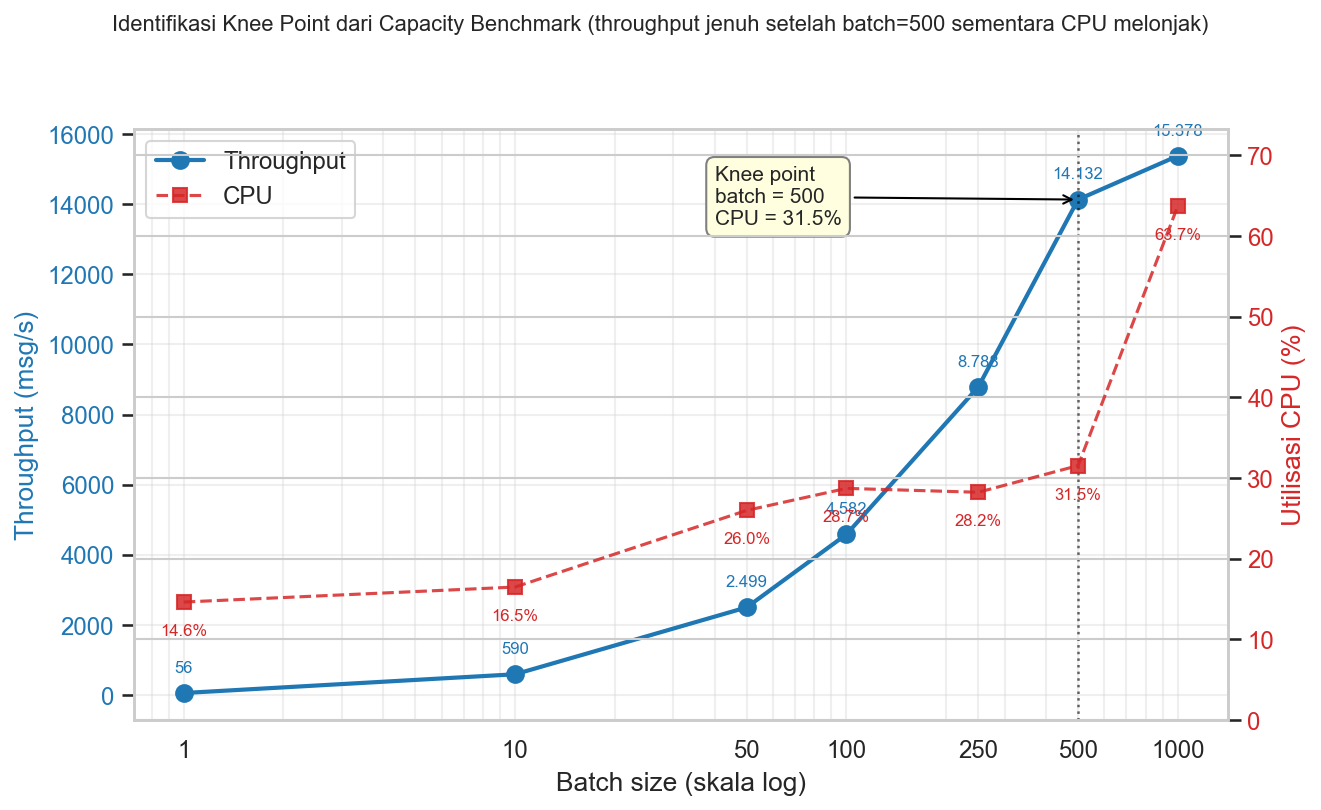
\includegraphics[width=0.85\textwidth]{IV_R10__knee_point.png}
    \caption{Identifikasi \emph{knee point} dari hasil \emph{capacity benchmark}}
    \label{fig:knee-point}
\end{figure}

\subsection{Penentuan Rentang \emph{Batch Size}}
\label{sec:batch-range}

Rentang \emph{batch size} diturunkan dari dua batasan fisik menggunakan Bryson's rule.
Bryson's rule adalah kaidah perancangan dalam kontrol optimal yang menetapkan nilai bobot
atau batasan berdasarkan rentang operasional yang dapat diterima, bukan dari penalaan
heuristik (Bryson dan Ho, 1975).
Pada konteks ini, kaidah tersebut diterapkan untuk menentukan batas atas \emph{batch size}
agar parameter kontrol selalu berada dalam wilayah operasi yang aman.
Setiap batasan memberikan jumlah dokumen maksimum per \emph{batch} yang masih aman, dan yang
mengikat adalah yang paling kecil di antara keduanya.

\begin{enumerate}
\item \textbf{Batasan memori:}
$\text{batch\_max}_{\text{mem}} = \lfloor J \times \alpha / d \rfloor$,
dengan $J = 512$~MB (\emph{heap}), $\alpha = 0{,}10$ (fraksi heap untuk \emph{bulk buffer}),
dan $d = \text{\docsizeKB}$~KB (ukuran dokumen terukur).
Hasilnya $\text{batch\_max}_{\text{mem}} = 113\,197$ dokumen.

\item \textbf{Batasan CPU:}
$\text{batch\_max}_{\text{cpu}} = C_{\text{limit}} \times 1000 / t_{\text{index}}$,
dengan $C_{\text{limit}} = 1{,}0$~core dan $t_{\text{index}} = 0{,}393$~ms/dok, yaitu waktu
rata-rata yang dibutuhkan Elasticsearch untuk mengindeks satu dokumen pada kondisi \emph{bulk},
diukur dari kolom $t\_\text{index}$ pada Tabel~\ref{tab:capacity-benchmark}.
Hasilnya $\text{batch\_max}_{\text{cpu}} = 2\,545$ dokumen.

\item \textbf{Batasan efektif:}
$\text{batch\_max} = \min(113\,197,\; 2\,545) \times 0{,}80 = \batchmaxCap$.
Karena CPU jenuh jauh lebih cepat daripada memori (2\,545 jauh lebih kecil dari 113\,197),
CPU menjadi batasan yang mengikat.
\emph{Batch} di atas 2\,545 hanya akan menambah waktu pemrosesan tanpa benar-benar menambah
\emph{throughput}, dan justru berisiko menyebabkan antrean penuh di tahap berikutnya.
Faktor keamanan 0,80 menyisakan ruang untuk \emph{garbage collection} dan proses \emph{merge}.

\item \textbf{Batas bawah:}
$\text{batch\_min} = \lceil t_{\text{conn}} / t_{\text{index}} \rceil = \lceil 1/0{,}39 \rceil = \batchminCap$,
dengan $t_{\text{conn}} = 1$~ms adalah estimasi biaya tetap pengiriman satu permintaan
\emph{bulk} HTTP pada koneksi \emph{keep-alive} (tidak termasuk TCP \emph{handshake}
yang sudah terjadi sebelumnya).
Nilai ini konsisten dengan observasi bahwa pada \emph{batch} = 1, overhead pengiriman
mendominasi waktu pengindeksan aktual, sehingga mengirim setidaknya 3 dokumen per
permintaan sudah cukup untuk menyeimbangkan biaya koneksi.
Nilai ini adalah titik di mana \emph{overhead} koneksi melebihi manfaat pemrosesan \emph{batch}.
\end{enumerate}

Rentang \emph{batch size} yang terjustifikasi adalah $[\batchminCap,\; \batchmaxCap]$.

\subsection{Penentuan Rentang \emph{Poll Interval}}
\label{sec:poll-range}

Rentang \emph{poll interval} ditentukan dari dua arah.

\begin{enumerate}
\item \textbf{Batas bawah (floor):}
$\text{poll\_min} = t_{\text{fetch}} + \text{batch\_mid} \times t_{\text{index}} + t_{\text{overhead}}$,
dengan $t_{\text{fetch}} = \text{\tfetchms}$~ms (waktu \emph{round-trip} Kafka yang terukur),
$\text{batch\_mid} = (\batchmaxCap + \batchminCap)/2 \approx 1019$, $t_{\text{index}} = 0{,}393$~ms/dok,
dan $t_{\text{overhead}} = 8$~ms adalah total biaya tetap per siklus \emph{poll} di luar waktu
\emph{fetch} dan pengindeksan, mencakup overhead \emph{consumer} Kafka, pengiriman \emph{bulk} HTTP,
dan \emph{parsing} respons.
Hasilnya: $\text{poll\_min} = 203 + 1019 \times 0{,}393 + 8 \approx \pollminCap$~ms.
Di bawah nilai ini, \emph{poll} selesai sebelum data dari Kafka siap, sehingga hanya membuang sumber daya.

\item \textbf{Batas atas (ceiling):}
$\text{poll\_max} = L_{\text{SLA}} - \text{batch\_mid} \times t_{\text{index}}$,
dengan $L_{\text{SLA}} = 2000$~ms (latensi end-to-end yang dapat diterima).
Hasilnya: $\text{poll\_max} = 2000 - 401 \approx \pollmaxCap$~ms.
Di atas nilai ini, latensi sinkronisasi melebihi batas yang dapat diterima.
\end{enumerate}

Rentang \emph{poll interval} yang terjustifikasi adalah $[\pollminCap,\; \pollmaxCap]$~ms.

\subsection{Penetapan Titik Operasional Nominal ($u_{\text{nom}}$)}

Titik nominal $u_{\text{nom}} = [\text{batch\_nom},\; \text{inv\_poll\_nom}]$ dipilih sebagai
titik keseimbangan yang memberikan kapasitas cukup tanpa mendekati batas saturasi CPU.

\begin{enumerate}
\item \textbf{batch\_nom = 250.}
Dari hasil \emph{benchmark}, \emph{batch}~=~250 menghasilkan \emph{throughput} 8.788~msg/s dengan
CPU 28\%, yakni di bawah \emph{knee point} (batch~=~\kneepoint, CPU~=~\kneeCpu\%).
Titik ini memiliki ruang untuk naik menuju \emph{knee point} jika antrean menumpuk,
sekaligus ruang untuk turun jika sumber daya tertekan.

\item \textbf{inv\_poll\_nom = 5{,}0 (poll = 200~ms).}
\emph{Poll interval} 200~ms mendekati $t_{\text{fetch}} = \text{\tfetchms}$~ms.
Pada \emph{poll} $\geq t_{\text{fetch}}$, setiap siklus \emph{poll} memiliki peluang tinggi menemukan
data baru (efisiensi \emph{polling} $= \min(1,\; t_{\text{fetch}} / \text{poll}) = 1{,}0$).
\emph{Poll} lebih cepat dari $t_{\text{fetch}}$ hanya akan membuang siklus CPU.
\end{enumerate}

\section{Eksperimen Open-Loop dan Identifikasi Sistem}

\subsection{Prosedur Eksperimen}

Eksperimen \emph{open-loop} dilakukan menggunakan grid 10$\times$10 dengan
spasi logaritmik dalam rentang yang telah ditetapkan.
Nilai \emph{batch size} yang diuji adalah \{3, 6, 13, 26, 54, 112, 232, 478, 987, 2036\} dan
\emph{poll interval} \{604, 673, 750, 836, 931, 1037, 1156, 1288, 1435, 1599\}~ms.
Spasi logaritmik dipilih karena respons sistem (terutama \emph{throughput}) menuju saturasi
terhadap kenaikan \emph{batch size}.

Setiap kombinasi kontrol diaplikasikan selama 60 detik setelah pra-pengisian antrean,
kemudian diikuti periode \emph{settling} 10 detik.
Total menghasilkan \openloopsamples{} sampel dari \openloopsteps{} langkah.

Variabel state yang dicatat adalah panjang antrean (\emph{queue\_length}),
utilisasi CPU, utilisasi memori, dan operasi I/O tulis.
Latensi dicatat sebagai variabel observasi saja dan tidak dimasukkan ke dalam vektor state,
karena pengujian sebelumnya menunjukkan bahwa latency di vektor state menyebabkan LQR menekan
\emph{batch size} secara berlebihan (\emph{batch collapse}).

Variabel kontrol yang divariasikan adalah \emph{batch size} dan \emph{inv\_poll\_interval}
($= 1000 / \text{poll\_ms}$).
Penggunaan \emph{inv\_poll\_interval} sebagai variabel kontrol (bukan \emph{poll\_interval})
mempertahankan hubungan yang lebih linier antara variabel ini dan \emph{throughput},
karena \emph{throughput} proporsional dengan frekuensi \emph{polling}, bukan intervalnya.

\subsection{Kualitas Model Identifikasi}

Model state-space $\mathbf{x}_{k+1} = A\mathbf{x}_k + B\mathbf{u}_k$ diestimasi menggunakan
regresi kuadrat terkecil (\emph{least squares}).
Sebelum estimasi, data difilter untuk membuang fase \emph{settle} (transien antar
konfigurasi) dan sampel dengan antrean nol (\emph{queue exhausted}).
Data tersisa dibagi menjadi 80\% sebagai data training dan 20\% sebagai data uji, dengan
pembagian dilakukan per kombinasi parameter \emph{(batch, poll)} untuk mencegah kebocoran
temporal antar himpunan.
Matriks $A$ dan $B$ kemudian diestimasi dari data training, dan kualitas fit ($R^2$) dihitung
pada data tersebut (\emph{in-sample fit}).
Nilai $R^2$ merepresentasikan seberapa baik model linier $A\mathbf{x}_k + B\mathbf{u}_k$
menjelaskan transisi state pada data training.

\begin{table}[H]
    \centering
    \caption{Kualitas fit model state-space per variabel}
    \label{tab:sysid-fit}
    \renewcommand{\arraystretch}{1.4}
    \begin{tabular}{|l|c|l|}
    \hline
    \textbf{Variabel State} & \textbf{$R^2$} & \textbf{Interpretasi} \\
    \hline
    Queue length & 0,994 & Sangat baik (mendekati integrator sempurna) \\
    \hline
    Utilisasi CPU & 0,694 & Cukup \\
    \hline
    Operasi I/O & 0,206 & Rendah \\
    \hline
    Utilisasi memori & 0,316 & Rendah (dinamika didominasi siklus GC JVM, kurang responsif terhadap perubahan batch size dan poll interval) \\
    \hline
    \end{tabular}
\end{table}

$R^2$ memori yang rendah konsisten dengan fakta bahwa heap JVM dikelola secara internal oleh
\emph{garbage collector} dan hampir tidak terpengaruh oleh \emph{batch size} atau
\emph{poll interval}.
Meski demikian, memori tetap dimasukkan ke dalam vektor state dengan bobot kecil pada matriks
$Q$ agar deviasi yang ekstrem tetap diperhitungkan dalam fungsi biaya, walaupun model linier
tidak dapat memprediksi dinamikanya dengan akurat.

\subsection{Koreksi Matriks B dari Data Kapasitas}

Matriks B yang diperoleh dari eksperimen \emph{open-loop} dengan eksitasi acak menunjukkan masalah
pada baris \emph{queue}: $B[\text{queue}, \text{batch}]$ bernilai positif pada estimasi awal,
yang secara fisik tidak masuk akal (batch besar seharusnya menguras antrean, bukan memperbesarnya).
Penyebabnya adalah \emph{confounding}: \emph{batch size} berkorelasi dengan besarnya pra-pengisian
antrean dalam prosedur eksperimen, sehingga regresi linier menangkap hubungan yang tidak kausal.

Untuk mengatasi hal ini, baris $B[\text{queue}, :]$ dikoreksi menggunakan data \emph{capacity benchmark}:

\begin{equation}
B[\text{queue}, \text{batch}] = -\frac{(\text{tput}(\mu_b + \sigma_b) - \text{tput}(\mu_b)) \cdot \Delta t}{\sigma_q}
\end{equation}

\begin{equation}
B[\text{queue}, \text{inv\_poll}] = -\frac{\text{tput}(\mu_b) \cdot (\text{eff}(\mu_p + \sigma_p) - \text{eff}(\mu_p)) \cdot \Delta t}{\sigma_q}
\end{equation}

dengan $\text{tput}(\cdot)$ adalah fungsi \emph{throughput} yang diinterpolasi dari data benchmark,
$\text{eff}(\cdot) = \min(1,\; t_{\text{fetch}} / \text{poll\_ms})$ adalah efisiensi \emph{polling},
$\mu_b = 130$, $\sigma_b = 75$ adalah mean dan standar deviasi \emph{batch} dari sysid,
$\mu_p = 5{,}0$, $\sigma_p = 3{,}0$ adalah mean dan standar deviasi \emph{inv\_poll},
$\sigma_q = 10.000$ adalah standar deviasi \emph{queue}, dan $\Delta t = 1$~detik.

Nilai yang dihasilkan adalah $B[\text{queue}, \text{batch}] = -0{,}21$ dan
$B[\text{queue}, \text{inv\_poll}] \approx 0$ (karena pada titik nominal \emph{poll} $\approx t_{\text{fetch}}$,
efisiensi sudah jenuh pada 1,0 sehingga penambahan \emph{inv\_poll} tidak meningkatkan \emph{throughput}).

Implikasi dari $B[\text{queue}, \text{inv\_poll}] \approx 0$ bagi DARE adalah bahwa kanal
\emph{inv\_poll} tidak berkontribusi pada drainase antrean, sehingga seluruh upaya koreksi
antrean dialokasikan ke kanal \emph{batch size}.
Ini menghasilkan gain $K$ yang lebih agresif pada \emph{batch}, sesuai dengan perilaku yang diinginkan.

\section{Rancangan Matriks Biaya LQR}

\subsection{Matriks R (Penalti Usaha Kontrol)}

Matriks $R$ dirancang menggunakan \emph{Bryson's rule} berbasis rentang operasional:

\begin{equation}
R_{ii} = \frac{R_{\text{base}}}{(\Delta u_{i,\max,\text{norm}})^2}
\end{equation}

dengan $\Delta u_{i,\max} = \max(u_{i,\max} - u_{i,\text{nom}},\; u_{i,\text{nom}} - u_{i,\min})$
adalah maksimum simpangan dari nominal, dan $\Delta u_{i,\max,\text{norm}} = \Delta u_{i,\max} / \sigma_{u_i}$
adalah simpangan tersebut dalam satuan normalisasi.

Dengan rentang dari \emph{capacity benchmark}:
$\Delta u_{\text{batch},\max} = \max(2036 - 250,\; 250 - 3) = 1786$ dan
$\Delta u_{\text{inv\_poll},\max} = \max(10 - 5,\; 5 - 0{,}625) = 5$,
serta $\sigma_{\text{batch}} = 75$ dan $\sigma_{\text{inv\_poll}} = 3$,
diperoleh:

\begin{equation}
R = R_{\text{base}} \cdot \text{diag}\!\left(\frac{1}{(1786/75)^2},\; \frac{1}{(5/3)^2}\right)
= 1{,}0 \cdot \text{diag}(1{,}76 \times 10^{-3},\; 0{,}36)
\end{equation}

Nilai $R[\text{batch}] \ll R[\text{inv\_poll}]$ mencerminkan fakta bahwa rentang operasional
\emph{batch size} ($\sim 2000$) jauh lebih besar daripada rentang \emph{inv\_poll} ($\sim 5$),
sehingga perubahan \emph{batch} ``lebih murah'' secara proporsional dan DARE dapat menggunakannya
lebih leluasa.

\subsection{Matriks Q (Penalti Deviasi State)}

Tiga preset matriks Q dirancang menggunakan \emph{Bryson's rule} pada ruang ternormalisasi,
untuk skenario prioritas yang berbeda.
Latensi tidak dimasukkan sebagai state (hanya sebagai variabel observasi), sehingga vektor state
adalah $\mathbf{x} = [\text{queue, cpu, mem, io}]^T$.
Diagonal Q dinyatakan sebagai bobot tanpa dimensi karena perhitungan biaya dilakukan pada ruang
$z$-score, sehingga rasio antar bobot mencerminkan prioritas relatif.

Setiap elemen diagonal $Q$ diturunkan dari Bryson's rule pada ruang ternormalisasi sebagai:

\begin{equation}
Q_{ii} = \left( \frac{\sigma_i}{\Delta x_{i,\text{maks}}} \right)^2 \times m_i
\label{eq:q-bryson}
\end{equation}

dengan $\sigma_i$ adalah standar deviasi ruang operasional (lihat Tabel~\ref{tab:lqr-norm}),
$\Delta x_{i,\text{maks}}$ adalah deviasi maksimum yang dapat diterima sistem, dan $m_i$ adalah
\emph{multiplier} yang menyatakan prioritas relatif antar preset.
Pemilihan $\Delta x_{i,\text{maks}}$ untuk masing-masing variabel state ditampilkan pada
Tabel~\ref{tab:q-input}.

\begin{table}[H]
    \centering
    \caption{Parameter input penurunan $Q_\text{base}$ menggunakan Bryson's rule}
    \label{tab:q-input}
    \renewcommand{\arraystretch}{1.4}
    \begin{tabular}{|l|r|r|p{6cm}|}
    \hline
    \textbf{Variabel} & \textbf{$\sigma_i$} & \textbf{$\Delta x_{i,\text{maks}}$} & \textbf{Justifikasi $\Delta x_\text{maks}$} \\
    \hline
    queue\_length & 5000 & 5000 & Deviasi sebesar satu standar deviasi sudah dianggap batas yang ketat untuk antrean \\
    \hline
    cpu\_util & 25 & 30 & Sedikit di atas standar deviasi, mencerminkan toleransi lonjakan CPU singkat \\
    \hline
    mem\_util & 20 & 100 & Memori kurang responsif terhadap aksi kontrol sehingga deviasi besar masih dapat ditoleransi \\
    \hline
    io\_write\_ops & 40 & 50 & Sekitar 1{,}25 standar deviasi, sesuai rentang p95 yang teramati \\
    \hline
    \end{tabular}
\end{table}

Substitusi nilai-nilai tersebut menghasilkan vektor $Q_\text{base}$:

\begin{align*}
Q_\text{base, queue} &= (5000/5000)^2 = 1{,}000 \\
Q_\text{base, cpu}   &= (25/30)^2     = 0{,}694 \\
Q_\text{base, mem}   &= (20/100)^2    = 0{,}040 \\
Q_\text{base, io}    &= (40/50)^2     = 0{,}640
\end{align*}

Tiga preset diperoleh dengan mengalikan $Q_\text{base}$ dengan vektor \emph{multiplier} $m$
yang menggeser prioritas antar variabel.
Nilai 4 dipilih karena memberikan perbedaan bobot yang cukup besar untuk menghasilkan perilaku
kontrol yang berbeda secara nyata, namun tetap dalam orde besaran yang sama agar matriks $K$
yang dihitung tetap stabil secara numerik.
Tabel~\ref{tab:lqr-q-presets} merangkum kombinasi tersebut.

\begin{table}[H]
    \centering
    \caption{Preset matriks $Q$ sebagai $Q_\text{base} \times m$ dan prioritas relatif}
    \label{tab:lqr-q-presets}
    \renewcommand{\arraystretch}{1.4}
    \begin{tabular}{|c|c|l|c|}
    \hline
    \textbf{Preset} & \textbf{Multiplier $m$} & \textbf{Diagonal Q} & \textbf{Prioritas relatif} \\
    \hline
    Q1 & [4, 1, 1, 1] & diag(4{,}000, 0{,}694, 0{,}040, 0{,}640) & 74\%, 13\%, 1 \%, 12 \% \\
    \hline
    Q2 & [1, 4, 4, 4] & diag(1{,}000, 2{,}778, 0{,}160, 2{,}560) & 15\%, 43\%, 2 \%, 39 \% \\
    \hline
    Q3 & [4, 4, 4, 4] & diag(4{,}000, 2{,}778, 0{,}160, 2{,}560) & 42\%, 29\%, 2 \%, 27 \% \\
    \hline
    \end{tabular}
\end{table}

Q1 memprioritaskan antrean sehingga kontroler menguras antrean lebih cepat dengan
konsekuensi pemakaian sumber daya yang lebih agresif.
Q2 membobot tinggi CPU dan IO, sehingga utilisasi sumber daya tetap rendah meskipun antrean
turun lebih lambat.
Q3 memperhatikan antrean dan sumber daya secara setara, cocok ketika kecepatan sinkronisasi
penting tanpa mengorbankan stabilitas sumber daya.

Bobot memori tetap kecil di seluruh preset karena memori dikelola oleh \emph{garbage collector}
JVM dan hampir tidak dipengaruhi secara langsung oleh \emph{batch size} atau \emph{poll interval}.
Memasukkan bobot besar pada memori hanya akan menambah \emph{noise} pada sinyal kontrol.

\subsection{State Target dan Titik Nominal Kontrol}

State target $\mathbf{x}^*$ dipilih sebagai berikut:

\begin{table}[H]
    \centering
    \caption{State target dan justifikasi pemilihan}
    \label{tab:state-target}
    \renewcommand{\arraystretch}{1.4}
    \begin{tabular}{|l|r|l|}
    \hline
    \textbf{Variabel} & \textbf{Target} & \textbf{Justifikasi} \\
    \hline
    queue\_length & 0 & Kondisi ideal: tidak ada antrean tertunda \\
    \hline
    cpu\_util & 5\% & Mendekati \emph{baseline} CPU saat idle (\emph{one-sided}: hanya dihukum jika $>5\%$) \\
    \hline
    mem\_util & 50\% & Nilai tengah rentang operasional; \emph{one-sided} \\
    \hline
    io\_write\_ops & 30 ops/s & Nilai median dari data historis; \emph{one-sided} \\
    \hline
    \end{tabular}
\end{table}

Penalti \emph{one-sided} pada cpu, mem, dan io berarti variabel ini hanya dihukum jika nilainya
melebihi target (bukan juga ketika lebih rendah).
Hal ini mencerminkan realitas bahwa CPU rendah bukan masalah, melainkan CPU tinggi yang perlu dihindari.

\subsection{Normalisasi untuk Ruang Kerja LQR}
\label{sec:lqr-norm}

Saat eksperimen \emph{open-loop} dijalankan dengan antrean besar (0--200.000), standar deviasi
$\sigma_q = 10.000$ mencerminkan rentang yang sangat lebar.
Namun dalam operasi \emph{closed-loop} aktual, antrean hanya bergerak dalam kisaran 0--7.000
(persentil ke-95 = 7.049).

Jika normalisasi sysid digunakan apa adanya, maka kesalahan state $\Delta q = 5.000$ dalam ruang
normalisasi hanya bernilai $5.000/10.000 = 0{,}5$, sehingga aksi kontrol yang dihasilkan DARE
jauh lebih kecil dari yang dibutuhkan.
Akibatnya, LQR terlihat tidak responsif meskipun gain $K$-nya besar.

Untuk mengatasi hal ini, normalisasi LQR di-\emph{override} ke rentang operasional
\emph{closed-loop} yang aktual.
Pada tabel berikut, kolom \textbf{Target ($x^*$)} adalah titik referensi yang dijadikan pusat
normalisasi, bukan rata-rata empiris dari data.
Misalnya, target queue\_length adalah 0 karena kontroler ingin menggiring antrean ke nol,
bukan ke nilai rata-rata historisnya.
Standar deviasi tetap diturunkan dari rentang operasional aktual.

\begin{table}[H]
    \centering
    \caption{Normalisasi LQR (di-\emph{override} dari sysid ke rentang \emph{closed-loop})}
    \label{tab:lqr-norm}
    \renewcommand{\arraystretch}{1.4}
    \begin{tabular}{|l|r|r|l|}
    \hline
    \textbf{Variabel} & \textbf{Target ($x^*$)} & \textbf{Std} & \textbf{Justifikasi std} \\
    \hline
    queue\_length & \normQueueMean & \normQueueStd & $\text{p95}_{cl} / 1{,}645 \approx 4286$ dibulatkan ke 5000 \\
    \hline
    cpu\_util & 5,0 & 25,0 & $\text{p95}_{cl}(=50\%) / 2 = 25$ (mencakup 5--55\%) \\
    \hline
    mem\_util & 50,0 & 20,0 & Sama dengan sysid (p5--p95 $\approx$ 21--73\%) \\
    \hline
    io\_write\_ops & 30,0 & 40,0 & $\text{p95}_{cl}(=99) / 2{,}5 = 40$ (mencakup 0--100) \\
    \hline
    batch\_size & \normBatchMean & \normBatchStd & $\text{max\_useful}/4 = 2036/4 \approx 509$ dibulatkan ke 250 \\
    \hline
    inv\_poll\_interval & \normInvPollMean & \normInvPollStd & Std aktual CL = 1,7; dibulatkan ke 2,0 \\
    \hline
    \end{tabular}
\end{table}

Dengan normalisasi ini, kesalahan antrean 5.000 dalam ruang normalisasi bernilai
$5.000 / 5.000 = 1{,}0$ (satu standar deviasi), menghasilkan aksi koreksi \emph{batch} yang
proporsional dengan kebutuhan aktual.

\section{Hasil Eksperimen Closed-Loop}

\subsection{Setup Eksperimen}

Eksperimen \emph{closed-loop} dijalankan pada satu mesin uji berbasis prosesor AMD Ryzen
dengan seluruh komponen sistem dijalankan sebagai kontainer Docker.
Tumpukan komponen meliputi PostgreSQL sebagai \emph{write database}, Kafka dengan Debezium CDC
sebagai \emph{message broker}, sebuah \emph{message sink} sebagai pengkonsumsi event, dan
Elasticsearch sebagai \emph{read database}.

Untuk menguji robustness kontroler terhadap perubahan kapasitas sistem, eksperimen dijalankan
pada tiga variasi sumber daya Elasticsearch.
Konfigurasi penuh (\emph{Full}) mengalokasikan 2{,}0 CPU, 2048 MiB memori, dan JVM heap 1024 MB.
Konfigurasi setengah (\emph{Half}) menggunakan separuh dari semuanya, yaitu 1{,}0 CPU,
1024 MiB memori, dan JVM heap 512 MB.
Konfigurasi seperempat (\emph{Quarter}) digunakan sebagai kasus batas dengan 0{,}5 CPU,
512 MiB memori, dan JVM heap 256 MB.

Pada masing-masing konfigurasi diuji enam strategi pengendalian, yaitu Statik, Rule-Based,
PID, LQR-Q1, LQR-Q2, dan LQR-Q3.
Setiap kombinasi kontroler dan pola beban dijalankan satu kali pada lima pola, yaitu
\emph{step}, \emph{ramp}, \emph{impulse}, \emph{periodic\_step}, dan \emph{step\_low},
sehingga total terdapat 30 percobaan per konfigurasi sumber daya.

\subsection{Metrik Evaluasi: Fungsi Biaya $J$ dan Regret Ternormalisasi}

Perbandingan utama menggunakan fungsi biaya $J$ yang dihitung secara \emph{post-hoc} pada
seluruh sampel dalam jendela waktu yang ditetapkan.

\begin{equation}
J = \frac{1}{T} \sum_{k=1}^{T} \left[(\mathbf{x}_k - \mathbf{x}^*)^\top Q (\mathbf{x}_k - \mathbf{x}^*) + (\mathbf{u}_k - \mathbf{u}_{\text{nom}})^\top R (\mathbf{u}_k - \mathbf{u}_{\text{nom}})\right]
\end{equation}

Nilai $J$ yang lebih rendah berarti kontroler lebih dekat ke kondisi yang diinginkan.
\emph{Regret} ternormalisasi dihitung sebagai
$r = (J_{\text{controller}} - J_{\text{best}}) / J_{\text{best}}$,
dengan $J_{\text{best}}$ adalah nilai $J$ kontroler terbaik pada konfigurasi yang sama.
Nilai $r = 0$ berarti kontroler terbaik dan $r > 0$ berarti lebih tinggi dari terbaik
secara proporsional.

\subsection{Hasil Sumber Daya Penuh}
\label{sec:hasil-full}

Pada konfigurasi penuh, sistem mengonsumsi 1724 sampel dengan latensi rata-rata 1848~ms
di seluruh kontroler dan pola beban.
Tabel~\ref{tab:cost-J-full} menunjukkan rangkuman fungsi biaya $J$ rata-rata per kontroler
pada masing-masing preset $Q$, beserta \emph{regret} ternormalisasi rata-rata.

\begin{table}[H]
    \centering
    \caption{Nilai rata-rata fungsi biaya $J$ pada konfigurasi sumber daya penuh}
    \label{tab:cost-J-full}
    \renewcommand{\arraystretch}{1.4}
    \begin{tabular}{|l|r|r|r|r|}
    \hline
    \textbf{Kontroler} & \textbf{Q1 (Backlog)} & \textbf{Q2 (Resource)} & \textbf{Q3 (Balanced)} & \textbf{Regret} \\
    \hline
    Statik           & 240,1 & 833,6 & 851,9 & 2,477 \\
    \hline
    Rule-Based       & 147,2 & 374,4 & 412,3 & 0,785 \\
    \hline
    PID              & 95,8 & 268,1 & 296,8 & 0,180 \\
    \hline
    \textbf{LQR}     & \textbf{82,3} & \textbf{217,4} & \textbf{241,4} & \textbf{0,000} \\
    \hline
    \end{tabular}
\end{table}

LQR menghasilkan biaya terendah pada seluruh preset $Q$ dengan \emph{regret} 0{,}000.
PID berada di urutan kedua dengan \emph{regret} rata-rata 0{,}180, sementara Statik tertinggal
jauh dengan \emph{regret} 2{,}477.
Pada preset Q1\_backlog yang menempatkan prioritas tertinggi pada antrean, LQR (82,3) lebih
rendah dari PID (95,8) sebesar 14\% dan dari Statik (240,1) sebesar 66\%.

Pemecahan biaya per pola beban pada preset Q1 ditampilkan pada Gambar~\ref{fig:bar-pattern-full}.
Selisih antar kontroler paling kentara pada pola \emph{step} dan \emph{periodic\_step},
yaitu kondisi di mana antrean naik secara berkelanjutan sehingga kemampuan kontroler
menyesuaikan \emph{batch} sangat menentukan.

\begin{figure}[H]
    \centering
    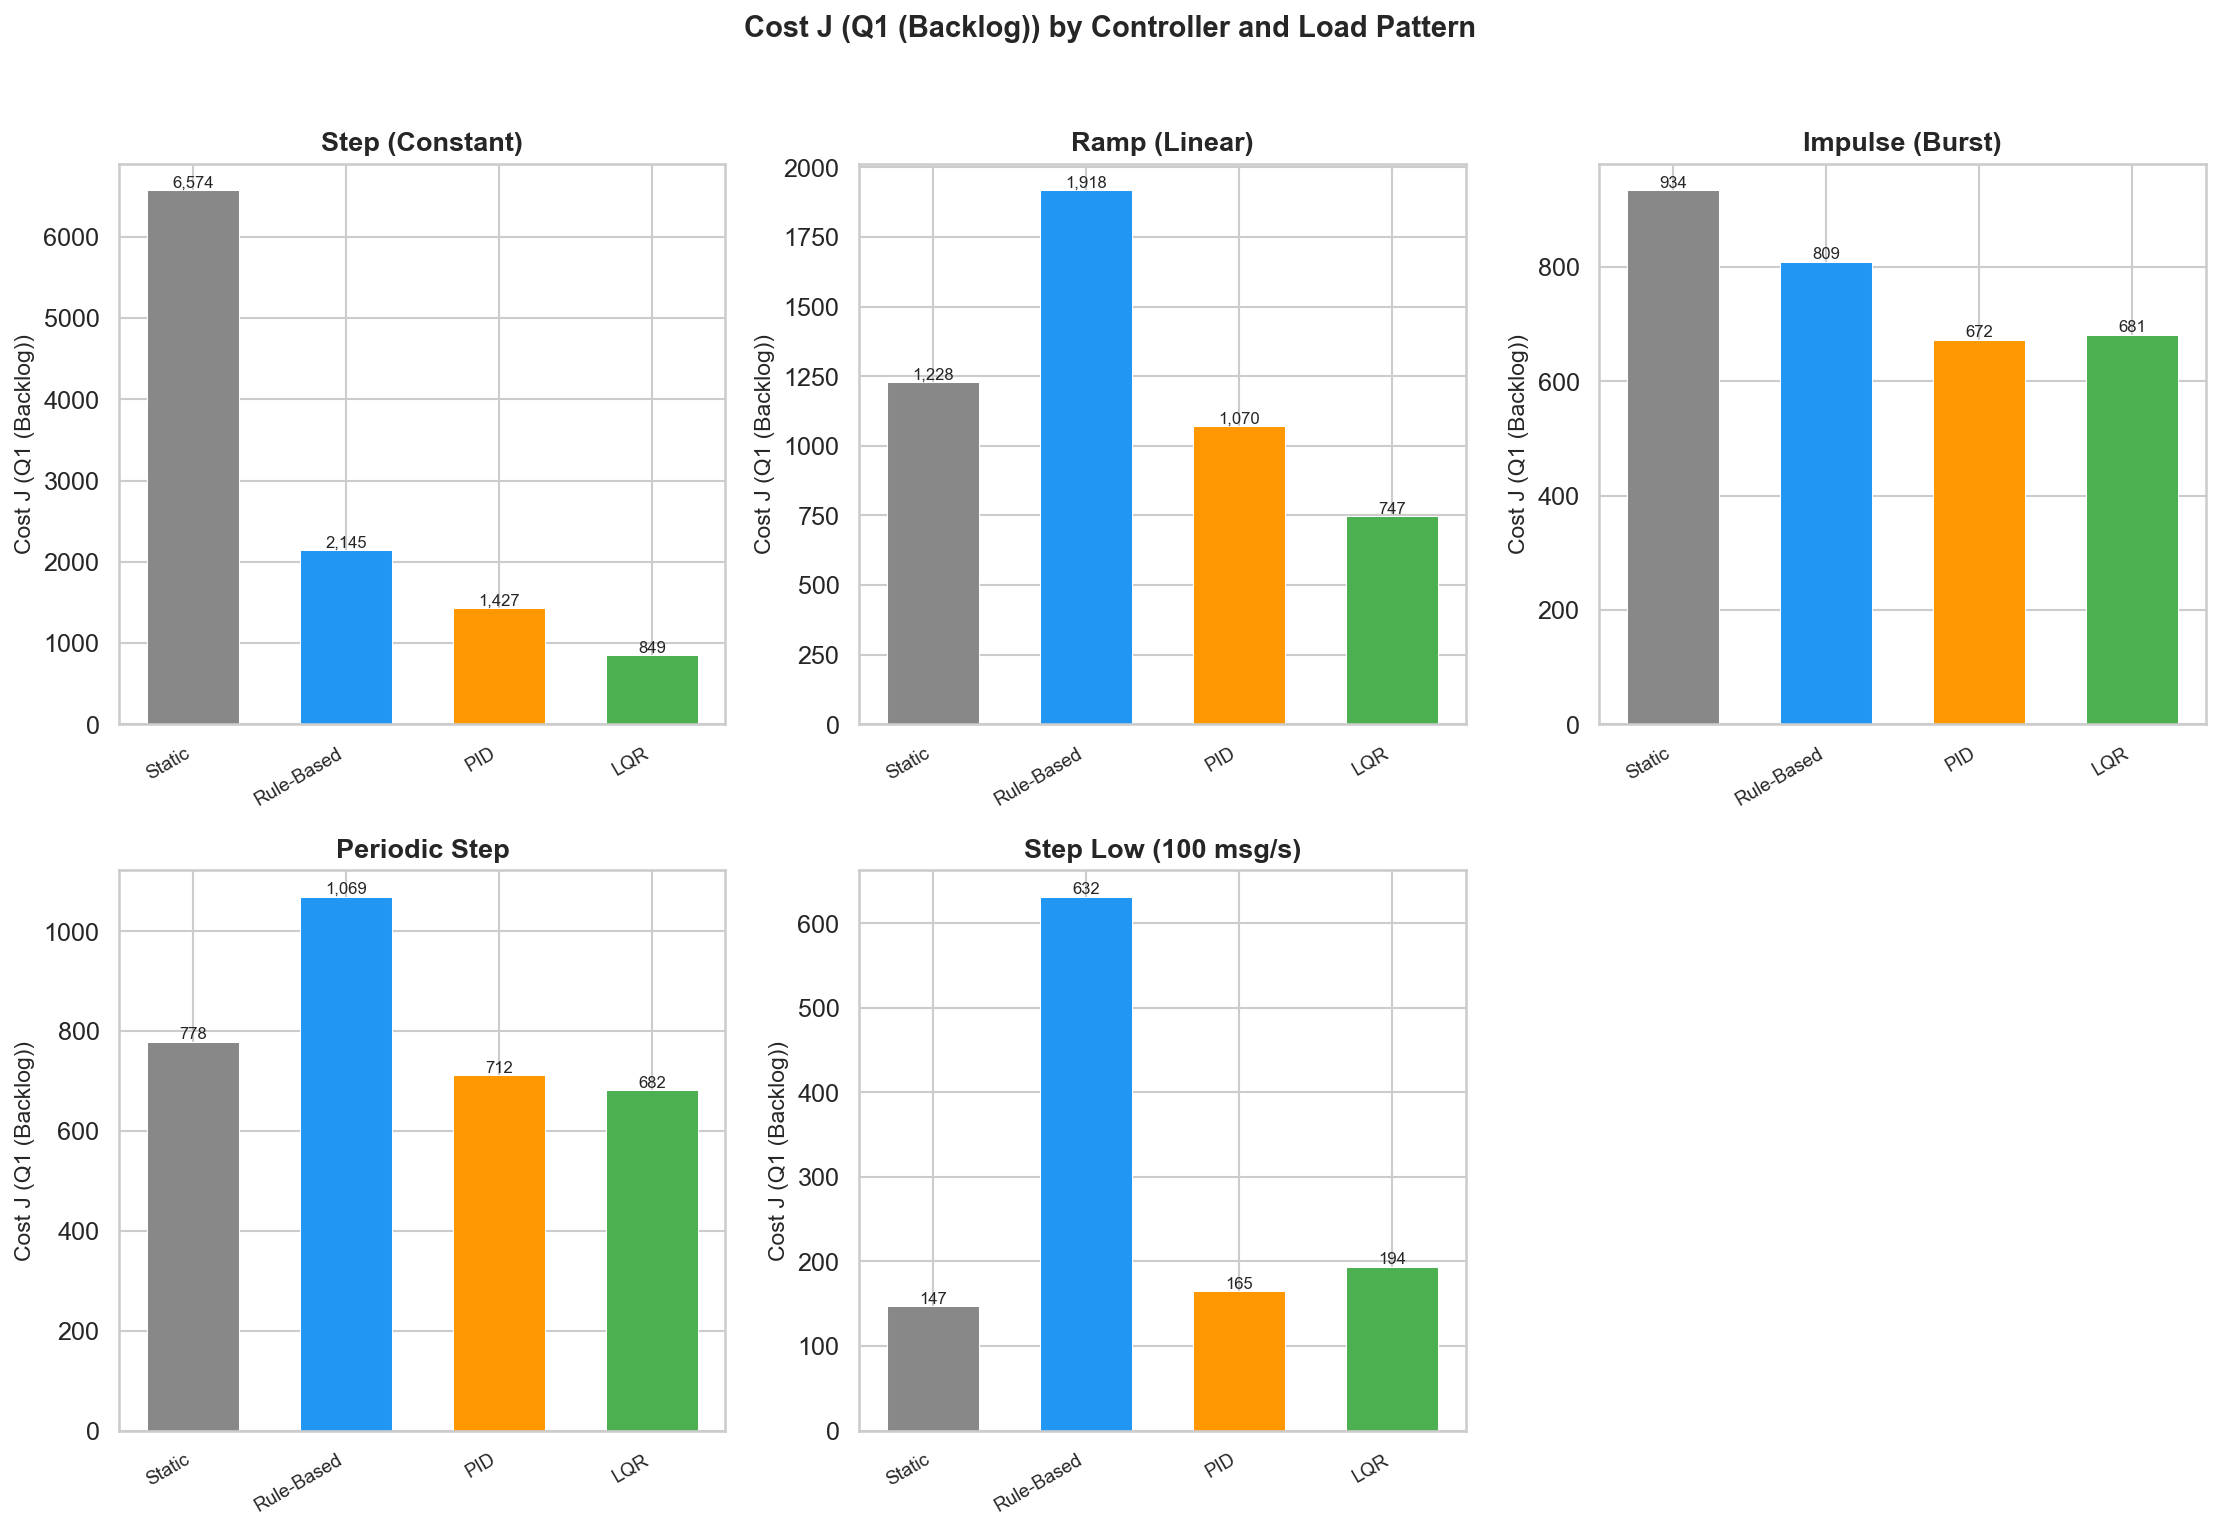
\includegraphics[width=0.85\textwidth]{IV_R2__bar_cost_pattern_full_Q1.png}
    \caption{Fungsi biaya $J$ per pola beban pada preset Q1 (sumber daya penuh)}
    \label{fig:bar-pattern-full}
\end{figure}

Throughput per kontroler pada preset Q1 ditunjukkan pada Gambar~\ref{fig:throughput-full}.
LQR mencapai \emph{throughput} tertinggi pada pola \emph{impulse}, di mana antrean melonjak
hingga 10.000 dan kontroler perlu mempercepat drainase secara agresif.

\begin{figure}[H]
    \centering
    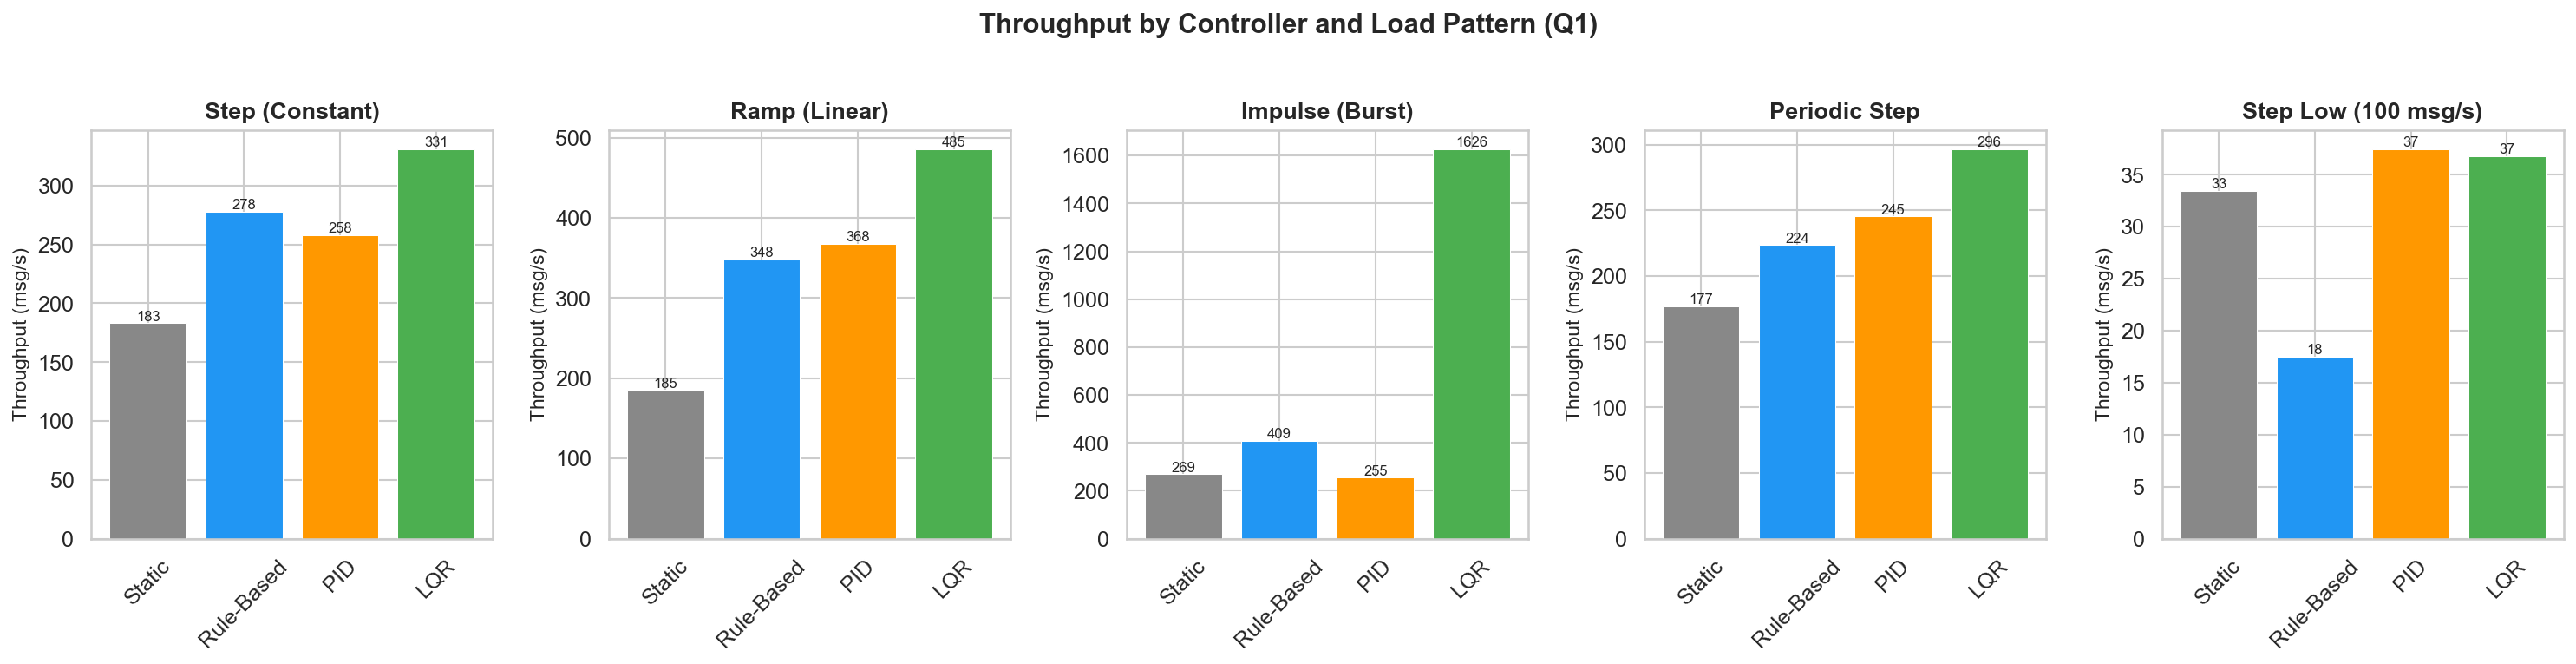
\includegraphics[width=0.85\textwidth]{IV_R3__bar_throughput_full_Q1.png}
    \caption{\emph{Throughput} per kontroler pada preset Q1 (sumber daya penuh)}
    \label{fig:throughput-full}
\end{figure}

Gambar~\ref{fig:timeseries-queue-full} menampilkan \emph{timeseries} antrean pada lima pola
beban dengan preset Q1.
LQR (warna hijau pada plot) konsisten menjaga antrean lebih rendah dibanding Statik dan
Rule-Based, terutama pada pola \emph{step} dan \emph{periodic\_step}.

\begin{figure}[H]
    \centering
    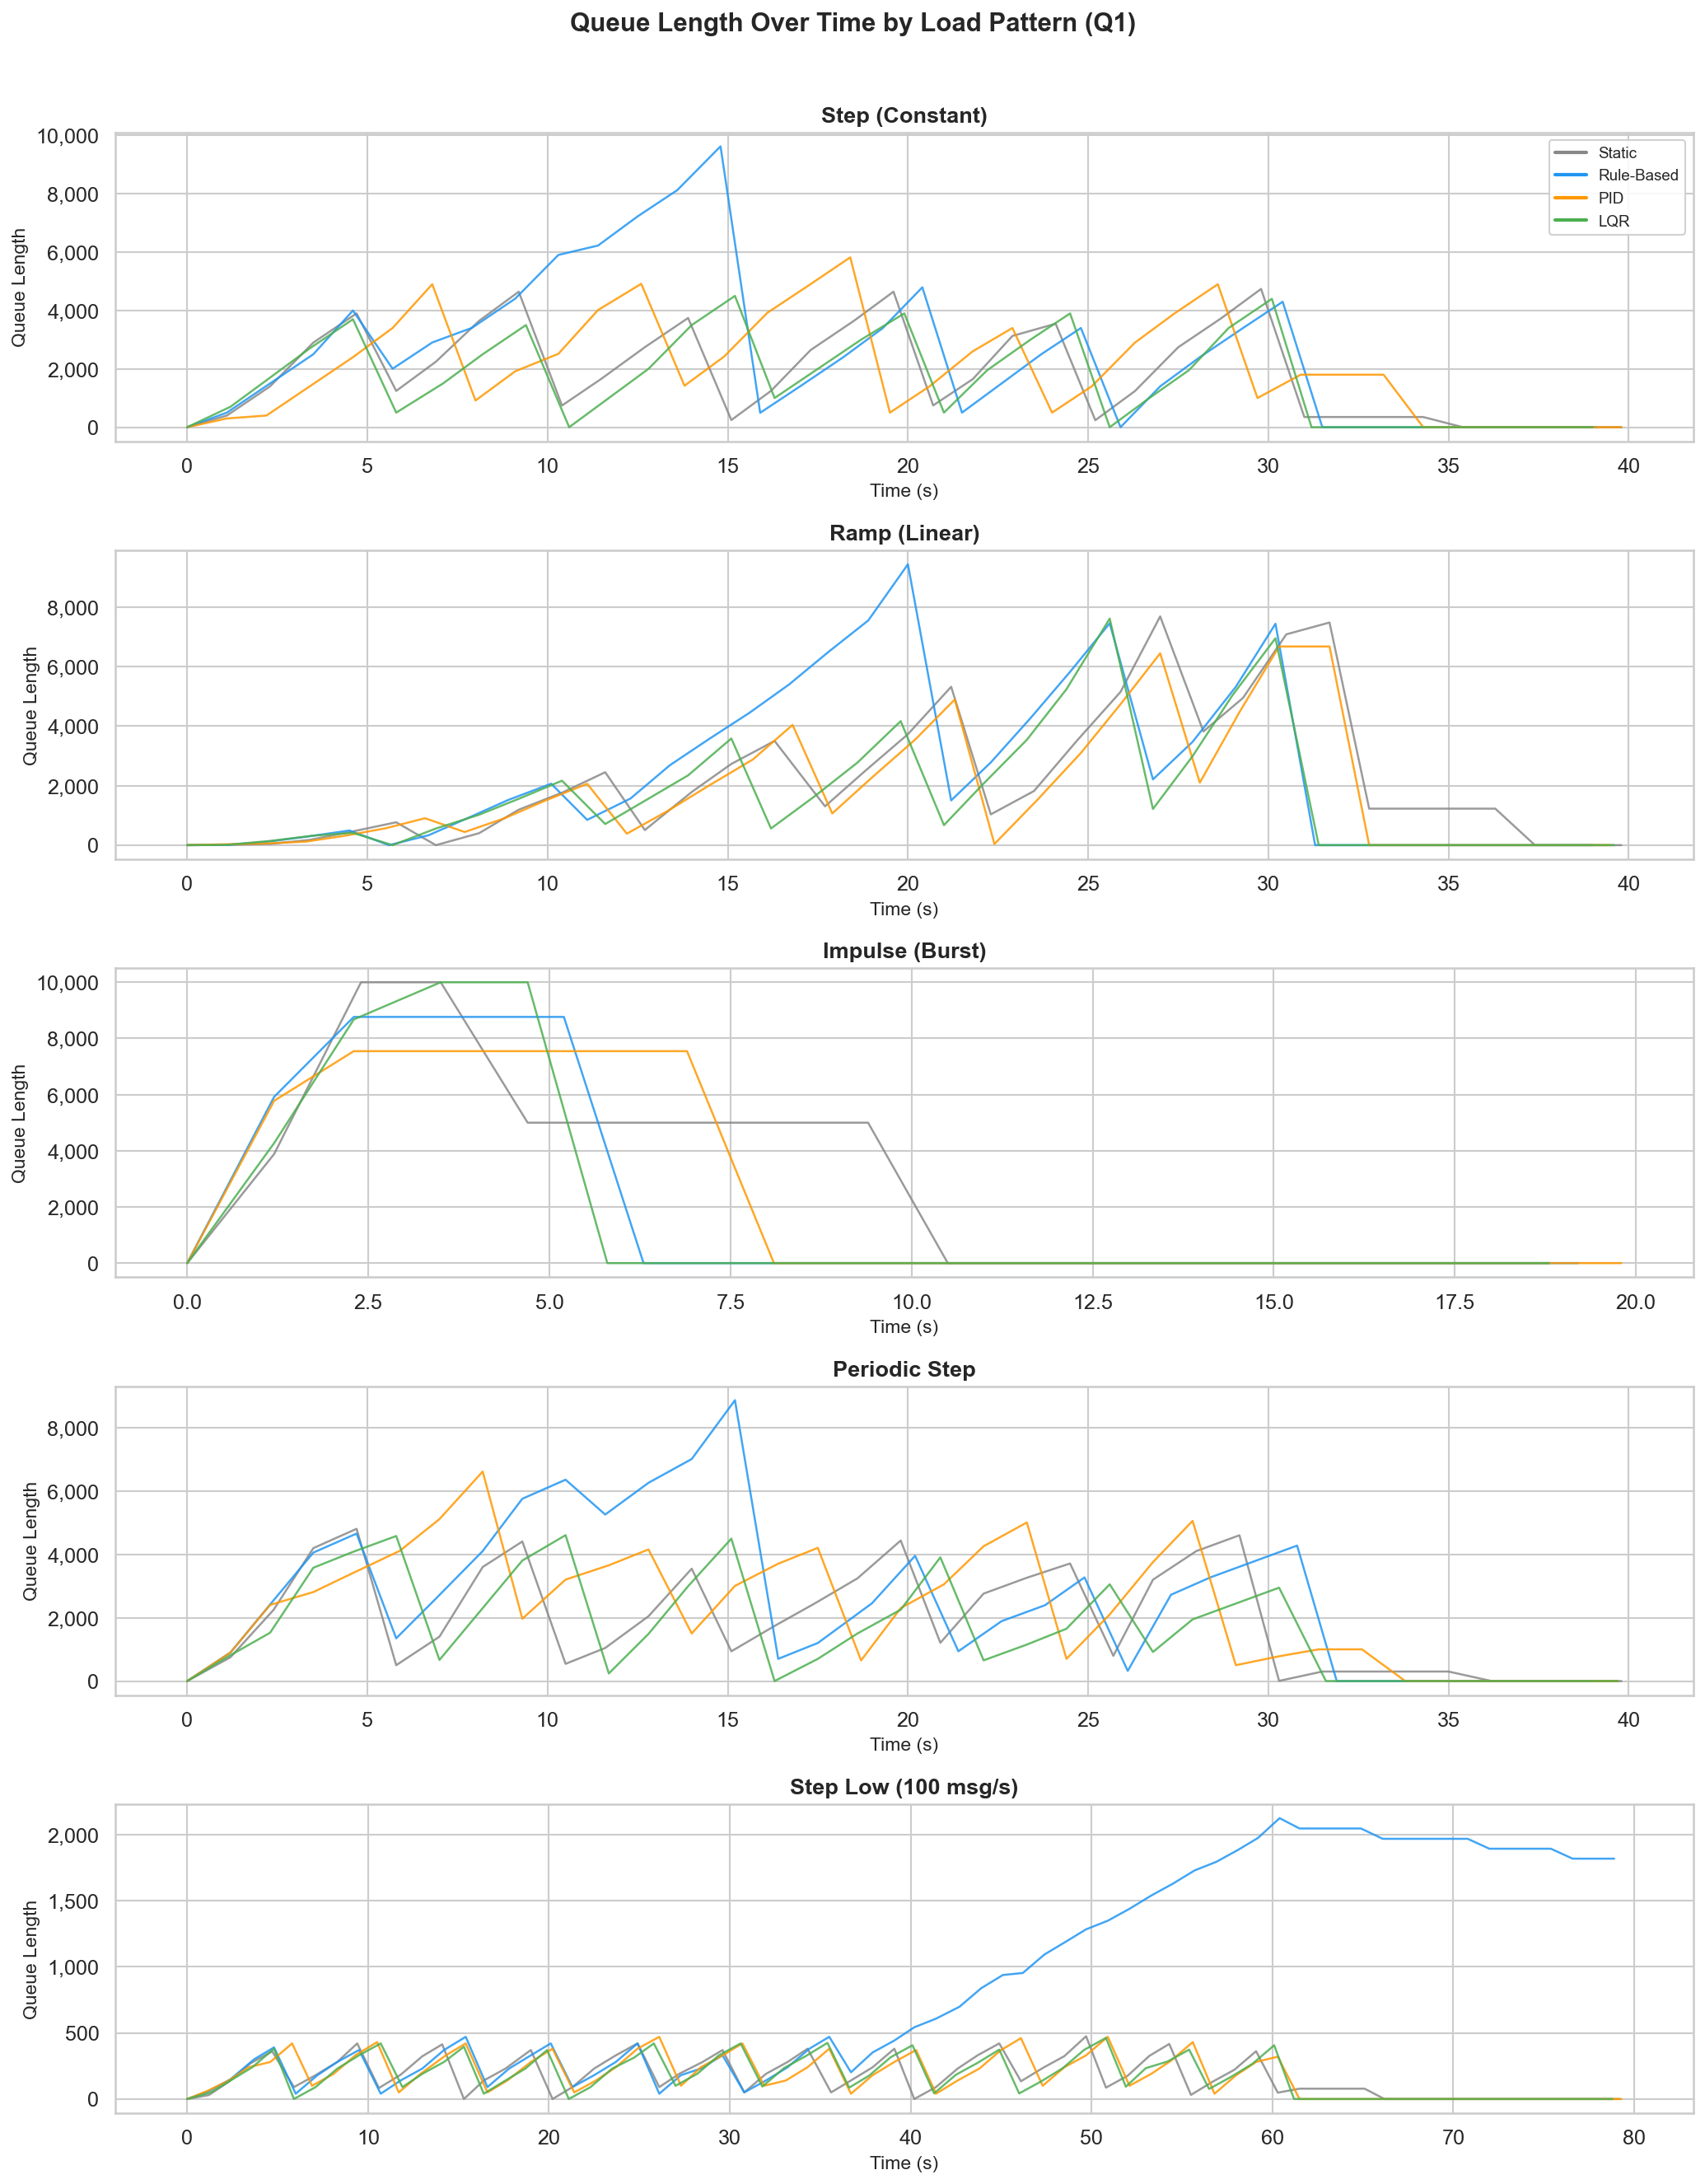
\includegraphics[width=\textwidth]{IV_R5__timeseries_queue_full_Q1.png}
    \caption{\emph{Timeseries} panjang antrean per kontroler pada lima pola beban (preset Q1, sumber daya penuh)}
    \label{fig:timeseries-queue-full}
\end{figure}

\subsection{Hasil Sumber Daya Setengah}
\label{sec:hasil-half}

Pada konfigurasi setengah, sistem mengonsumsi 1780 sampel dengan latensi rata-rata 2455~ms,
sekitar 1{,}3 kali latensi pada konfigurasi penuh.
Tabel~\ref{tab:cost-J-half} menunjukkan rangkuman fungsi biaya $J$ pada konfigurasi ini.

\begin{table}[H]
    \centering
    \caption{Nilai rata-rata fungsi biaya $J$ pada konfigurasi sumber daya setengah}
    \label{tab:cost-J-half}
    \renewcommand{\arraystretch}{1.4}
    \begin{tabular}{|l|r|r|r|r|}
    \hline
    \textbf{Kontroler} & \textbf{Q1 (Backlog)} & \textbf{Q2 (Resource)} & \textbf{Q3 (Balanced)} & \textbf{Regret} \\
    \hline
    Statik           & 157,8 & 483,7 & 513,3 & 1,418 \\
    \hline
    Rule-Based       & 154,2 & 386,5 & 432,9 & 1,101 \\
    \hline
    PID              & 87,0 & 226,1 & 254,7 & 0,150 \\
    \hline
    \textbf{LQR}     & \textbf{63,7} & \textbf{169,5} & \textbf{191,9} & \textbf{0,000} \\
    \hline
    \end{tabular}
\end{table}

Polanya sama dengan konfigurasi penuh, di mana LQR memberikan biaya terendah dan diikuti
oleh PID.
Yang menarik adalah jarak relatif antar kontroler.
Pada konfigurasi setengah, \emph{regret} Rule-Based menjadi 1{,}101 atau jauh lebih buruk
dibanding pada konfigurasi penuh yang hanya 0{,}785.
Ini menunjukkan bahwa Rule-Based semakin tertinggal saat sumber daya menipis, karena aturan
ambang batas yang statis tidak menyesuaikan diri terhadap kapasitas yang lebih kecil.

LQR justru tetap kompetitif dengan \emph{regret} 0{,}000 dan biaya absolut yang lebih rendah
dibanding versi penuh (63,7 vs 82,3 pada Q1).
Hal ini terjadi karena LQR menyesuaikan aksi kontrol berdasarkan kondisi sistem aktual,
sehingga ketika kapasitas berkurang, antrean terbangun lebih lambat dan kontroler memilih
batch yang lebih moderat tanpa kehilangan kemampuan drainase.

Gambar~\ref{fig:bar-pattern-half} menampilkan distribusi biaya per pola beban untuk
konfigurasi setengah, sedangkan Gambar~\ref{fig:timeseries-queue-half} menampilkan
\emph{timeseries} antrean.

\begin{figure}[H]
    \centering
    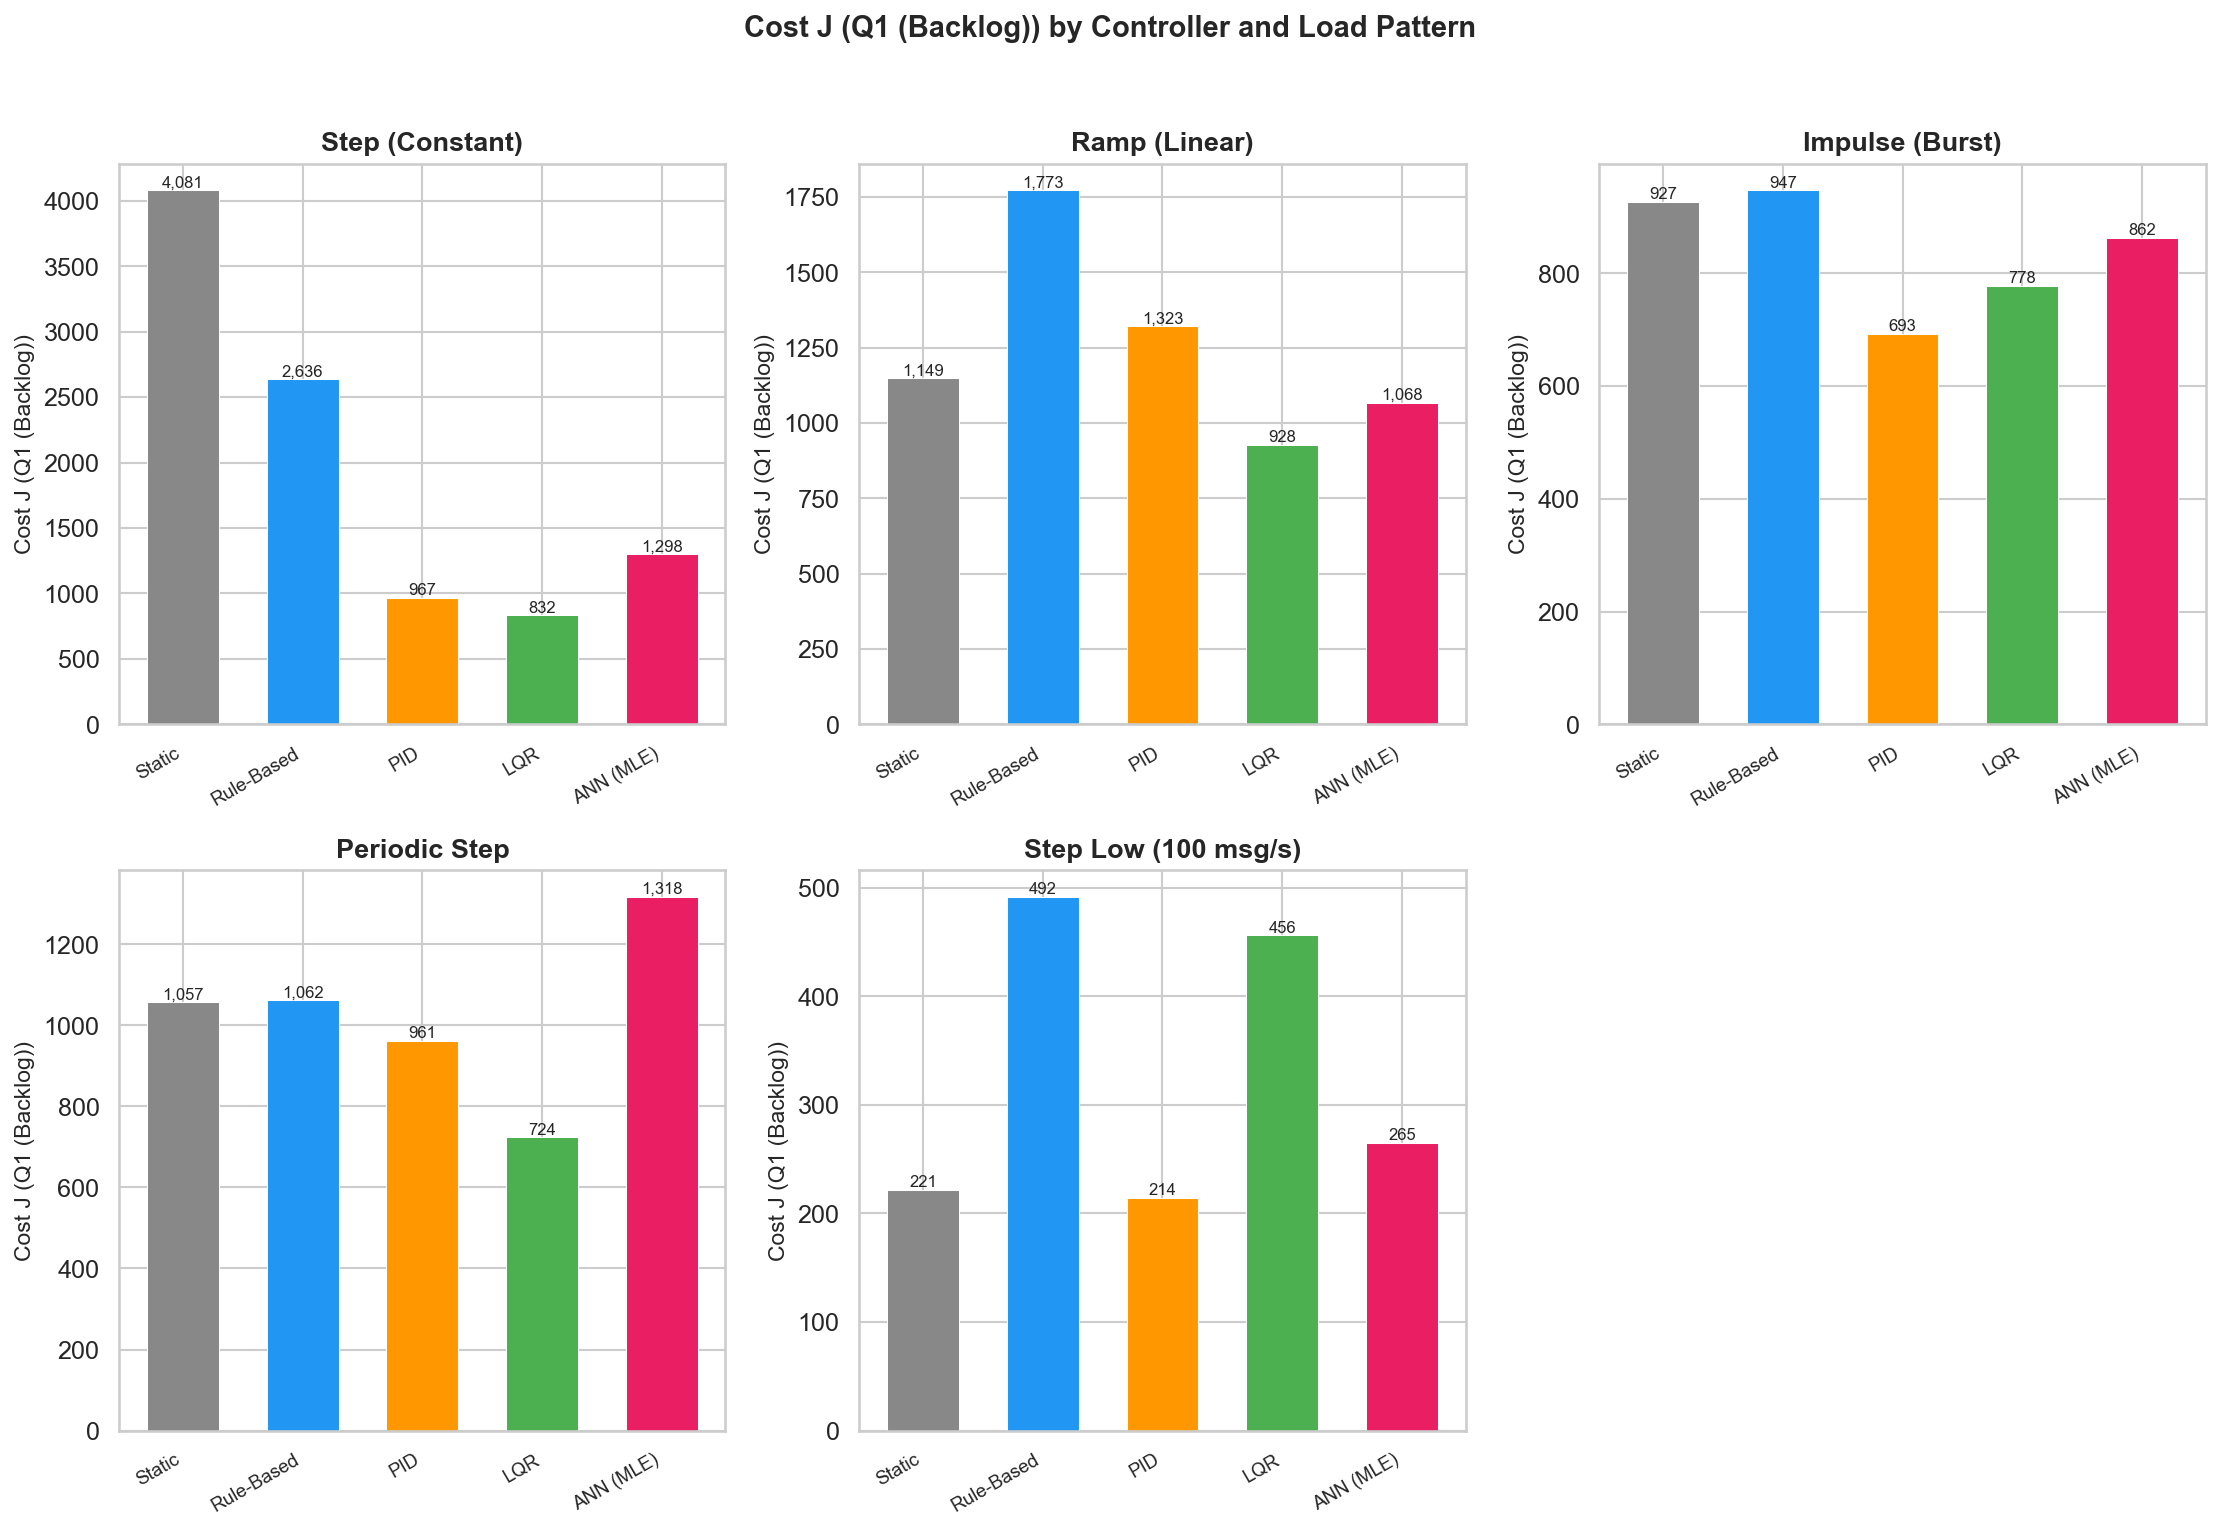
\includegraphics[width=0.85\textwidth]{IV_R7__bar_cost_pattern_half_Q1.png}
    \caption{Fungsi biaya $J$ per pola beban pada preset Q1 (sumber daya setengah)}
    \label{fig:bar-pattern-half}
\end{figure}

\begin{figure}[H]
    \centering
    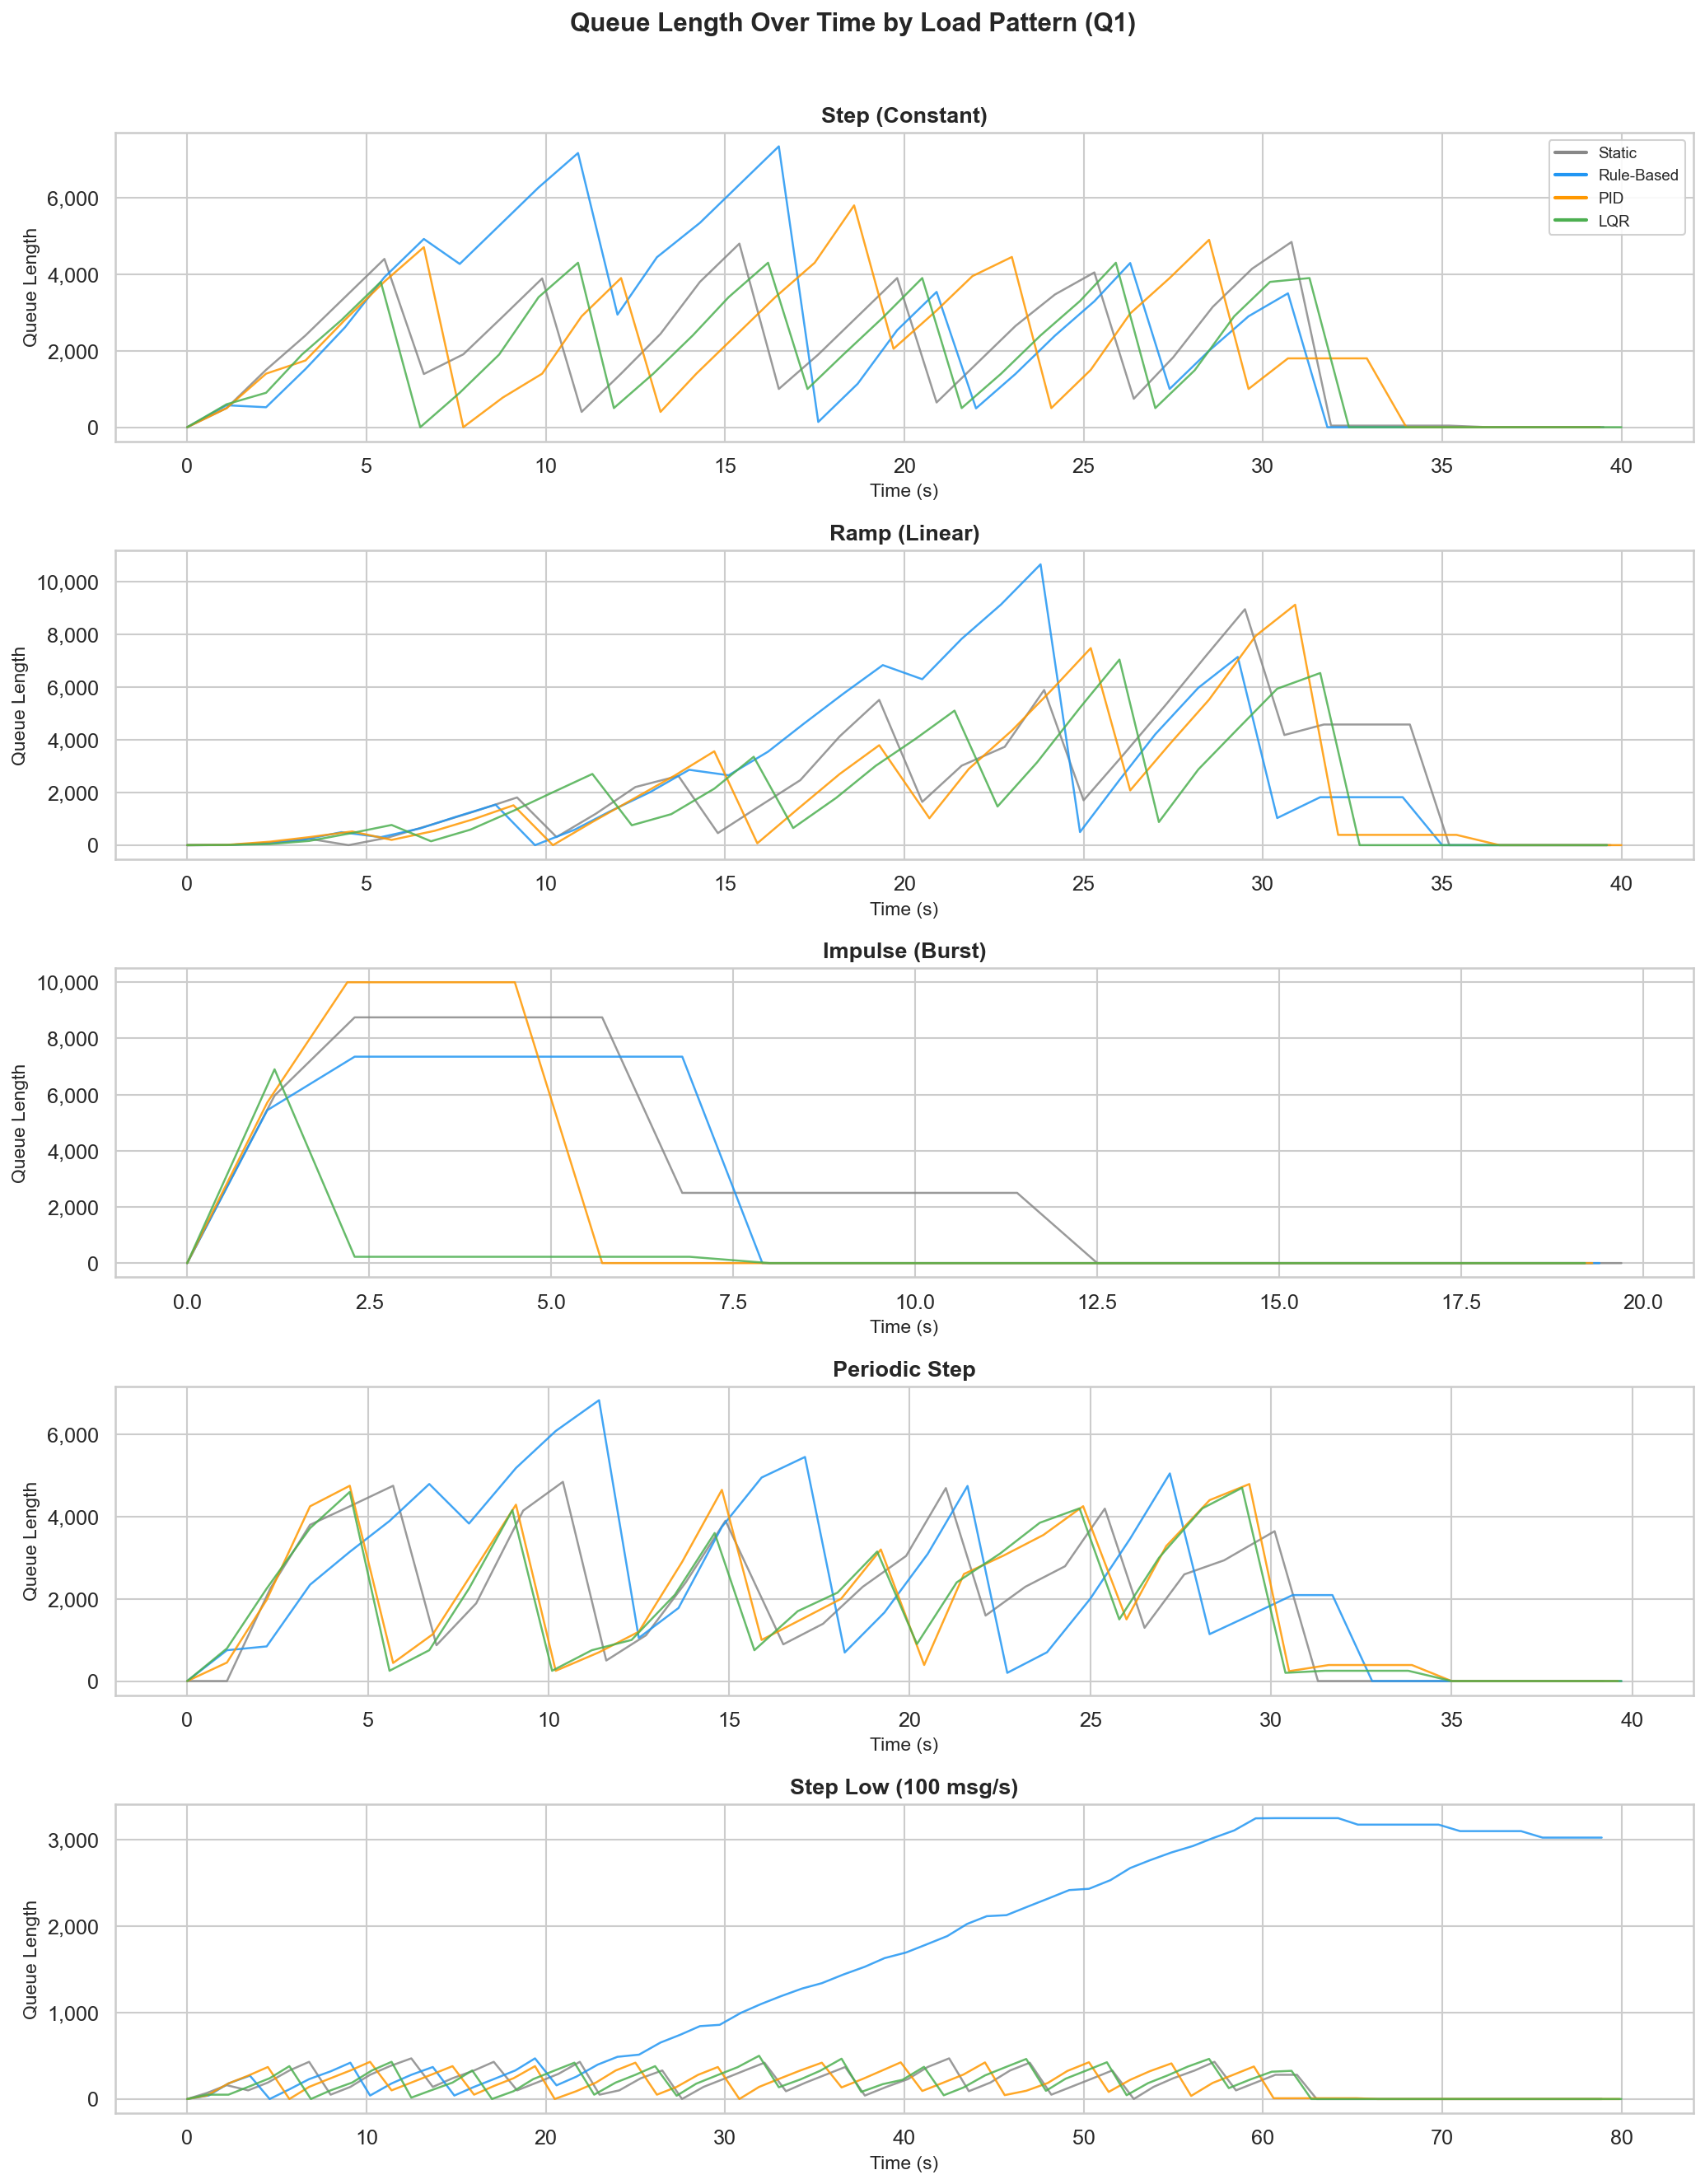
\includegraphics[width=\textwidth]{IV_R8__timeseries_queue_half_Q1.png}
    \caption{\emph{Timeseries} panjang antrean per kontroler pada lima pola beban (preset Q1, sumber daya setengah)}
    \label{fig:timeseries-queue-half}
\end{figure}

Tabel~\ref{tab:robustness} merangkum perubahan \emph{regret} antara dua konfigurasi.
Statik dan Rule-Based degradasi cukup tajam saat sumber daya menipis, sementara PID dan LQR
relatif stabil.
Bahkan, \emph{regret} Statik membaik dari 2{,}477 ke 1{,}418 saat sumber daya berkurang.
Anomali ini muncul karena \emph{regret} dinormalisasi terhadap kontroler terbaik, sehingga
ketika baseline LQR juga melemah secara absolut, jarak relatif terhadap LQR menyempit.
Yang penting adalah peringkat tetap konsisten yaitu LQR di posisi terbaik diikuti PID.

\begin{table}[H]
    \centering
    \caption{Perbandingan \emph{regret} rata-rata pada dua konfigurasi sumber daya}
    \label{tab:robustness}
    \renewcommand{\arraystretch}{1.4}
    \begin{tabular}{|l|r|r|}
    \hline
    \textbf{Kontroler} & \textbf{Regret (Penuh)} & \textbf{Regret (Setengah)} \\
    \hline
    Statik       & 2,477 & 1,418 \\
    \hline
    Rule-Based   & 0,785 & 1,101 \\
    \hline
    PID          & 0,180 & 0,150 \\
    \hline
    \textbf{LQR} & \textbf{0,000} & \textbf{0,000} \\
    \hline
    \end{tabular}
\end{table}

\subsection{Adaptasi Antar Preset Q}
\label{sec:adaptasi}

Salah satu karakteristik LQR yang membedakannya dari kontroler lain adalah kemampuannya
mengubah perilaku berdasarkan matriks bobot $Q$.
Gambar~\ref{fig:state-across-q} menunjukkan rata-rata variabel sistem untuk seluruh kontroler
pada tiga preset $Q$ yang berbeda, dengan baseline ditampilkan sebagai garis putus-putus
karena nilainya konstan terhadap $Q$.

\begin{figure}[H]
    \centering
    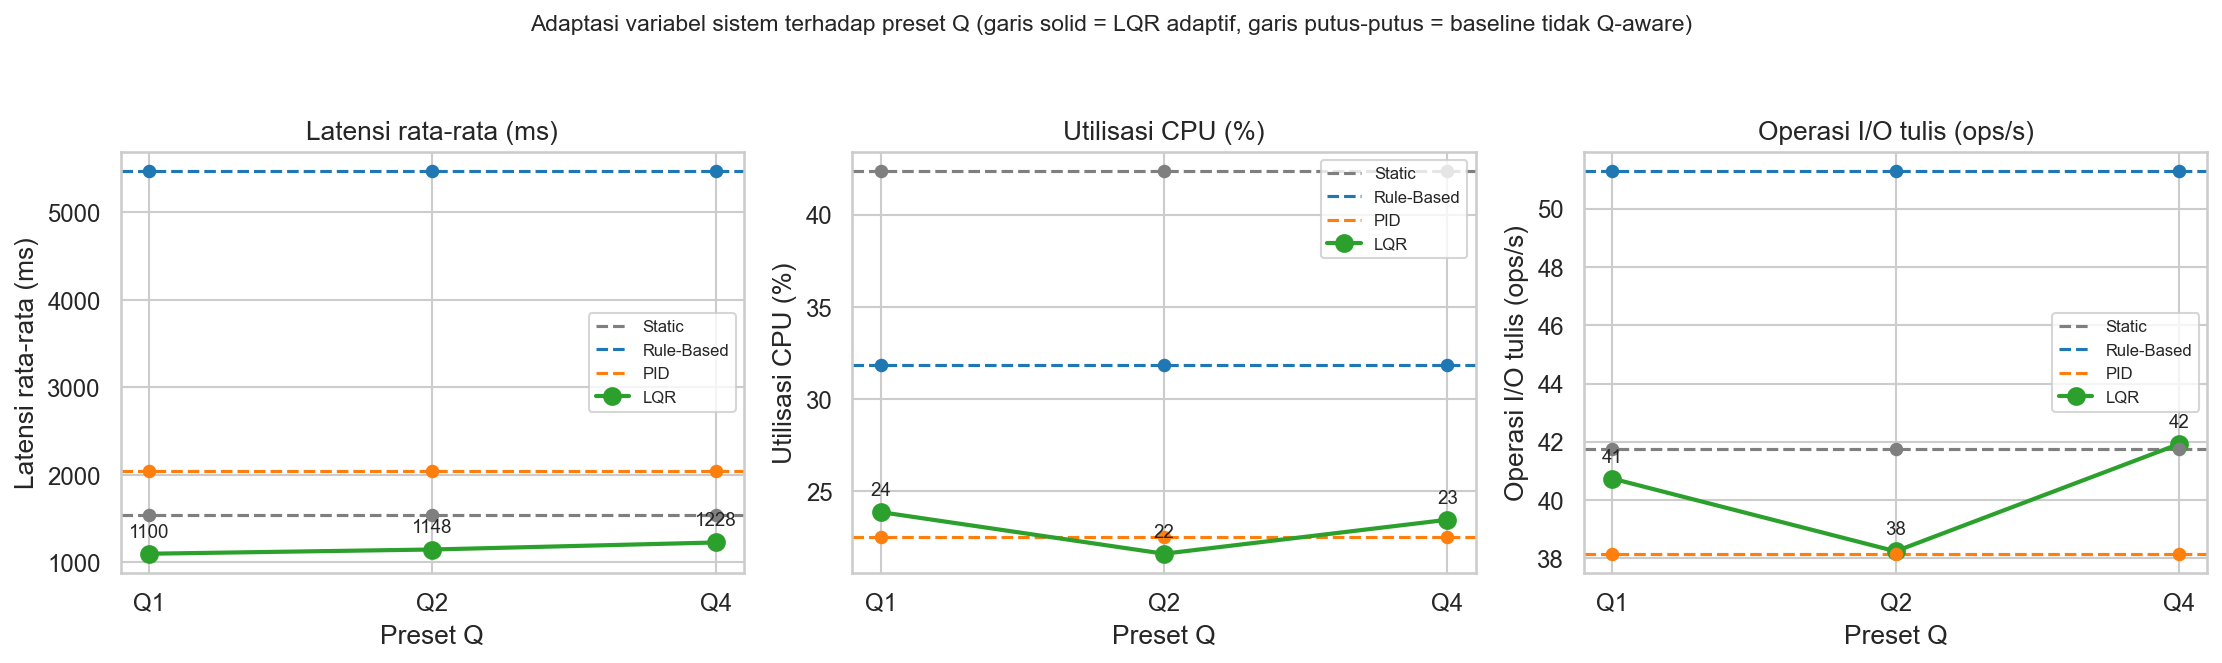
\includegraphics[width=\textwidth]{IV_R4__state_across_q_full.png}
    \caption{Rata-rata variabel sistem per kontroler pada tiga preset $Q$ (sumber daya penuh)}
    \label{fig:state-across-q}
\end{figure}

Pada panel latensi, LQR konsisten berada di tingkat terendah dengan pergeseran tipis dari
1100 ms pada Q1 ke 1228 ms pada Q3.
Pada panel utilisasi CPU, LQR-Q2 yang memprioritaskan penghematan sumber daya memberikan
nilai paling rendah (22\%) dibanding LQR-Q1 dan LQR-Q3.
Pada panel I/O, LQR-Q2 juga menunjukkan operasi tulis paling sedikit, sejalan dengan
prioritas resource pada preset tersebut.

Kontroler Statik, Rule-Based, dan PID tampil sebagai garis horizontal karena perilakunya
tidak ditentukan oleh $Q$.
Ketiganya tidak memiliki mekanisme untuk menyerap perubahan prioritas, sehingga menghasilkan
nilai variabel sistem yang sama untuk seluruh preset.
Inilah yang menjadi nilai utama LQR sebagai kontroler berbasis fungsi biaya, yaitu satu
implementasi dapat dikonfigurasi ulang untuk prioritas yang berbeda hanya dengan mengganti
matriks $Q$.

Variabel utilisasi memori tidak ditampilkan karena pembacaan dari kontainer Elasticsearch
menghasilkan nilai nol pada eksperimen ini, sehingga tidak dapat digunakan untuk membandingkan
adaptasi antar kontroler.

\subsection{Robustness Lintas Mesin dan Konfigurasi}
\label{sec:robustness}

Untuk menguji apakah keunggulan LQR bertahan pada kombinasi perangkat keras dan kapasitas
yang berbeda, eksperimen yang sama dijalankan pada empat kombinasi (dua mesin uji, masing-masing
dengan dua konfigurasi sumber daya).
Mesin pertama menggunakan AMD Ryzen sebagai host, sementara mesin kedua menggunakan Apple
Silicon.
Pada setiap mesin, Elasticsearch dijalankan pada konfigurasi penuh (2{,}0 CPU, 2 GiB memori,
heap 1 GiB) dan konfigurasi setengah (1{,}0 CPU, 1 GiB memori, heap 512 MiB).

Tabel~\ref{tab:cross-experiment} merangkum nilai $J$ rata-rata setiap kontroler pada keempat
eksperimen.
Nilai dihitung dengan merata-ratakan cost $J$ atas lima pola beban dan tiga preset $Q$ untuk
setiap kontroler, dengan varian LQR dipasangkan pada preset $Q$ yang sesuai.

\begin{table}[H]
    \centering
    \caption{Cost $J$ rata-rata per kontroler pada empat eksperimen}
    \label{tab:cross-experiment}
    \renewcommand{\arraystretch}{1.4}
    \begin{tabular}{|l|r|r|r|r|}
    \hline
    \textbf{Kontroler} & \textbf{Mac Full} & \textbf{Mac Half} & \textbf{Ryzen Full} & \textbf{Ryzen Half} \\
    \hline
    Statik           & 962,4 & 4697,7 & 640,7 & 385,0 \\
    \hline
    Rule-Based       & 237,4 & 2805,8 & 317,2 & 324,4 \\
    \hline
    PID              & 63,2 & 3575,7 & 209,7 & 175,9 \\
    \hline
    \textbf{LQR}     & \textbf{16,2} & \textbf{1254,2} & \textbf{177,9} & \textbf{159,6} \\
    \hline
    \end{tabular}
\end{table}

LQR memberikan cost $J$ terendah di seluruh empat eksperimen, sedangkan Statik selalu
menjadi yang tertinggi.
Pada Mac Half, biaya seluruh kontroler melonjak jauh lebih tinggi dibanding eksperimen lain,
yang menunjukkan bahwa kombinasi perangkat keras Mac dengan kapasitas terbatas menyulitkan
seluruh strategi untuk menjaga deviasi state.
Bahkan dalam kondisi sulit tersebut, LQR (1254,2) tetap setengah dari Statik (4697,7)
dan jauh di bawah PID (3575,7).

Gambar~\ref{fig:cross-experiment} menampilkan visualisasi yang sama dalam bentuk batang.
Setiap panel menggunakan skala mandiri karena nilai absolut $J$ berbeda jauh antar eksperimen,
sehingga skala bersama akan membuat perbedaan dalam panel kecil tidak terbaca.

\begin{figure}[H]
    \centering
    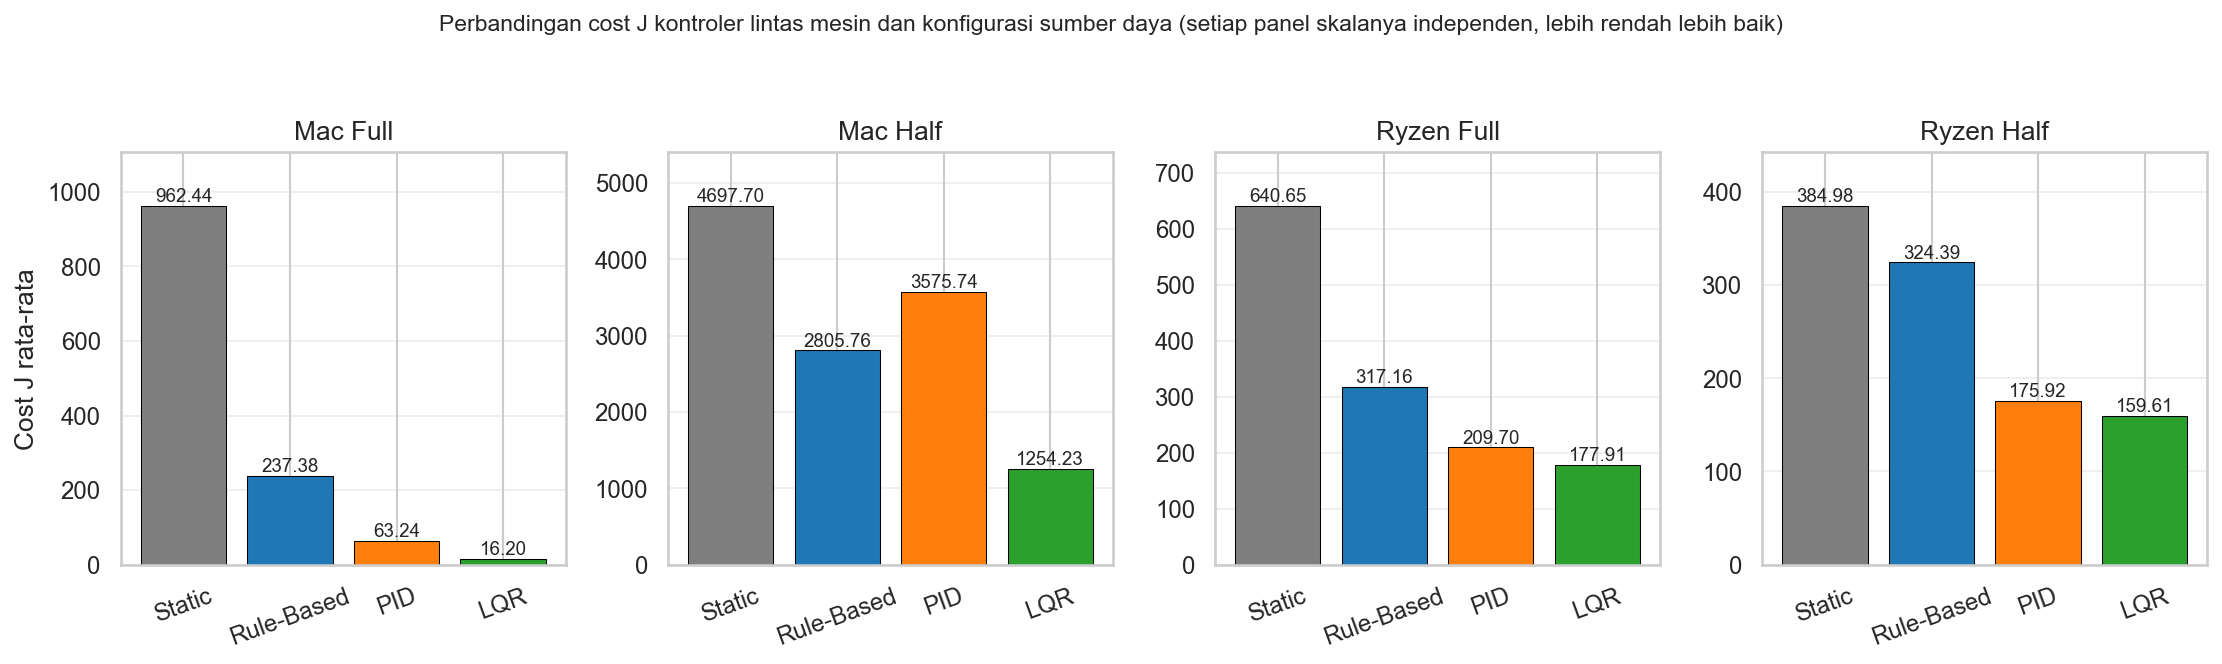
\includegraphics[width=\textwidth]{IV_R9__cross_experiment_cost.png}
    \caption[Cost J kontroler lintas empat eksperimen]{Cost $J$ rata-rata per kontroler pada empat eksperimen, dengan setiap panel berskala independen}
    \label{fig:cross-experiment}
\end{figure}

Perlu dicatat bahwa nilai $J$ absolut tidak dapat dibandingkan secara langsung antar mesin
karena matriks $Q$ untuk Mac dan Ryzen dikalibrasi terpisah dari hasil identifikasi sistem
masing-masing.
Yang konsisten adalah ranking dalam setiap eksperimen, di mana LQR selalu di urutan teratas.
Hal ini menunjukkan bahwa keunggulan LQR bukan artefak dari satu konfigurasi tertentu,
melainkan akibat langsung dari mekanisme pengendalian yang menggabungkan seluruh variabel
sistem ke dalam satu fungsi biaya.

\subsection{Kasus Batas pada Sumber Daya Quarter}
\label{sec:quarter}

Konfigurasi seperempat (\emph{Quarter}) dengan 0{,}5 CPU, 512 MiB memori, dan JVM heap 256 MB
diuji sebagai kasus batas untuk melihat perilaku sistem ketika kapasitas Elasticsearch tidak
lagi memadai.
Latensi rata-rata pada konfigurasi ini mencapai 6797~ms atau sekitar 3{,}7 kali latensi pada
konfigurasi penuh, yang menunjukkan bahwa Elasticsearch sudah dalam kondisi saturasi.
Pada kondisi ini, perbedaan antar kontroler menjadi kurang relevan karena bottleneck bergeser
dari pengaturan parameter ke kapasitas pemrosesan basis data itu sendiri.
Hasil pada konfigurasi Quarter tidak dilampirkan dalam bentuk tabel atau plot karena
karakteristiknya sebagai kasus degradasi yang tidak mencerminkan kondisi operasional yang ditargetkan.


% \chapter{Kesimpulan}

Bab ini memuat elaborasi dan rincian kesimpulan yang dituliskan pada abstrak. Saran untuk kajian lanjutan serta \textit{practical implication} dari kerja Mahasiswa S2 dapat dituliskan pada bab ini.
\blindtext
%----------------------------------------------------------------%

% Daftar pustaka
\blankpage
\addcontentsline{toc}{chapter}{Daftar Pustaka}

\chapter*{DAFTAR PUSTAKA}

\noindent CQRS, data diperoleh melalui situs internet: https://martinfowler.com/bliki/CQRS.html. Diunduh pada tanggal 6 Juni 2025.

\noindent Vogels, W. (2009). Eventually Consistent. \emph{Communications of the ACM}, 40--44.

\noindent Kindsoon, Munoye., Martinek, Péter (2023): A Simplified Approach to Distributed Message Handling in a CQRS Architecture, \emph{Acta Polytechnica Hungarica.}

\noindent Armağan, Özgür., Gören-Sümer, Leyla (2014): Feedback control for multi-resource usage of virtualized database server, \emph{Computers and Electrical Engineering.}

\noindent Pan, Wenping., Mu, Dejun., Wu, Hangxing., Yao, Lei (2008): Feedback Control-based QoS Guarantees in Web Application Servers, \emph{IEEE International Conference on High Performance Computing and Communications.}

\noindent Das, T., Zhong, Y., Stoica, I., Shenker, S., dan Zaharia, M. (2018): Adaptive stream processing using dynamic batch sizing, \emph{Proceedings of the ACM Symposium on Cloud Computing.}

\noindent Gong, Siqian., Yin, Beibei., Cai, Kai-yuan (2018): An Adaptive PID Control for QoS Management in Cloud Computing System, \emph{IEEE International Symposium on Software Reliability Engineering Workshops.}

\noindent Wu, Han., Shang, Zhiao., Guang, Peng., Wolter, Katinka (2020). A Reactive Batching Strategy of Apache Kafka for Reliable Stream Processing in Real-time, \emph{IEEE International Symposium on Software Reliability Engineering.}

\noindent ZangLong (2017). Improvement and Implementation of a High Performance CQRS Architecture, \emph{International Conference on Robots \& Intelligent System..}

\noindent Bailis, Peter., Venkataraman, Shivaram., Franklin, Michael J., Hellerstein, Joseph M., Stoica, Ion (2017). Probabilistically Bounded Staleness for Practical Partial Quorums, \emph{International Conference on Robots \& Intelligent System.}

\noindent Kindsoon, Munoye., Martinek, Péter (2020). Evaluation of Data Storage Patterns in Microservices Archicture, \emph{IEEE 15th International Conference of System of Systems Engineering}

\noindent Ogata, K. (2010). \emph{Modern Control Engineering} (5th ed.). Prentice Hall. 793--798

\noindent Kleppmann, M. (2017). \emph{Designing Data-Intensive Applications: The Big Ideas Behind Reliable, Scalable, and Maintainable Systems}. O'Reilly Media. 389-391

\noindent Ljung, L. (1999): \emph{System identification: Theory for the user}, 2nd ed., Prentice Hall, Upper Saddle River

\noindent Newman, S. (2015). \emph{Building Microservices: Designing Fine-Grained Systems}. O'Reilly Media. 193--198

\noindent Brewer, E. (2000). Towards Robust Distributed Systems. \emph{Proceedings of the Annual ACM Symposium on Principles of Distributed Computing (PODC)}.


% Setting judul lampiran
\titlespacing*{\chapter}{0pt}{0pt}{0pt}
\titlespacing*{\section}{0pt}{0pt}{*1}

% Setting judul anak lampiran
\titleformat*{\section}{\bfseries\normalsize}

% Index
\appendix
\input{chapters/appendix-1.tex}
\input{chapters/appendix-2.tex}

\end{document}

